\section{Proof of \cref{sec-gt-gc,prop:sec-gc-gc:rel_sat_cond_ac}}
\label{sec-proofs:prop:sec-gc-gc:rel_sat_cond_ac}
We prove the result for positive conditions at first and for non-positive conditions afterwards.
By induction over the structure of nested conditions:
\begin{center}
\begin{tikzpicture}[]
\fill (0,0) node[inner sep=1pt] (P) {$P$};
\fill (4,0) node[inner sep=1pt] (C) {$C$};
\fill (0,-3) node[inner sep=1pt] (G) {$G$};
\fill (.5,-1.5) node[inner sep=1pt] (P') {$P'$};
\fill (3,-1.5) node[inner sep=1pt] (C') {$C'$};
\fill (4.6,0) node [isosceles triangle, fill=gray!25,draw,minimum width=0.4cm, inner sep=1pt,rotate=180] (t) {};
\fill (5.05,0) node[inner sep=1pt] {$\ac_C$};
\fill (2,-.75) node[inner sep=1pt] (O) {$O$};
%
\fill (2.5,-1) node[inner sep=1pt] {$(1)$};
\fill (2,-.4) node[inner sep=1pt] {$(2)$};
\fill (.75,-.8) node[inner sep=1pt] {$(3)$};
%
{
\pgfsetarrowsend{latex}
\draw (P) -> node[fill=white,inner sep=1pt]{$\scriptstyle{a}$} (C);
\draw (P) -> node[fill=white,inner sep=1pt]{$\scriptstyle{p}$} (G);
\draw (C) edge[bend left=40] node[fill=white,inner sep=5pt]{$\scriptstyle{q}$} (G);
\draw (P) -> node[fill=white,inner sep=1pt]{$\scriptstyle{e_p}$} (P');
\draw (C) -> node[fill=white,inner sep=1pt]{$\scriptstyle{e'_p}$} (C');
\draw (P') -> node[fill=white,inner sep=1pt]{$\scriptstyle{m_p}$} (G);
\draw (C') -> node[fill=white,inner sep=5pt]{$\scriptstyle{m_q}$} (G);
\draw (P') -> node[fill=white,inner sep=5pt]{$\scriptstyle{a'}$} (C');
\draw (O) -> node[fill=white,inner sep=5pt]{$\scriptstyle{o_1}$} (C);
\draw (O) -> node[fill=white,inner sep=5pt]{$\scriptstyle{o_2}$} (P');
\draw (P) -> node[fill=white,inner sep=5pt]{$\scriptstyle{o_3}$} (O);
%
\pgfsetarrows{*-latex}
\pgfsetarrows{->>}
\pgfsetarrows{left hook-latex}
}
\end{tikzpicture}
\end{center}
\begin{description}
    \item[``$\Rightarrow$''] \textbf{Basis.}
    For $\ac_P=\true$, let $m_p \circ e_p=p$ be the extremal $\E$-$\M$ factorisation of $p$ with $(e_p,\true) \in \Inst(\ac_P)$.
    It holds that $m_p \models \true$ and therefore, $p \models \exists(e_p,\true)$ implying further that $p \models \ol{\ac}_P$.
    For $\ac_P=\exists(a\colon P \to C \in \M,\true)$, $p \models \ac_P$ implies that there is $q \in \M$ with $q \circ a=p$.
    Let $m_p \circ e_p=p$ be the extremal $\E$-$\M$ factorisation of $p \in \M$ with $e_p \in \M$ by $\M$-decomposition.
    We construct pullback $(o_1,o_2)$ over $(m_p,q)$ with $o_1,o_2 \in \M$, since, $\M$-morphisms $m_p,q \in \M$ are closed under pullbacks.
    We construct pushout $(1)$ with $a',e'_p \in \M$, since, $\M$-morphisms $o_1,o_2 \in \M$ are closed under pushouts.
    By effective pushouts, the induced morphism $m_q$ is in $\M$ with $m_q \circ a'=m_p$ and $m_q \models \true$ and therefore, $m_p \models \exists(a',\true)$.
    It remains to show that $\exists(a',\true)$ is in $\Merge(e_p,\ac_P)$ which would imply that $m_p \models \Merge(e_p,\ac_P)$ and furthermore, $p \models \ol{\ac}_P$ by \cref{rem:sec-gc-gc:schemata}.
    By the universal pullback property, there is $o_3$ with $(2)$ and $(3)$ commute.
    By $(1),(2)$ and $(3)$ commute, respectively, $(1)+(2)+(3)$ commutes.
    Furthermore, $a',e'_p \in \M$ and therefore, $e'_p \in \morO$ according to \cref{rem:sec-gt-M-adh:agraphs_atgi}.
    Moreover, pushout $(1)$ implies that $(a',e'_p)$ are jointly epimorphic and $\Merge(e'_p,\true)=\true$ by construction.
    \textbf{Hypothesis.}
    The result holds for conditions $\ac_C$ and $\ac_{P,i},i \in I$.
    \textbf{Step.}
    For $\ac_P=\exists(a\colon P \to C \in \M,\ac_C)$, we conclude for morphism $a$ like before with induced morphism $m_q \in \M$ and $m_q \circ e'_p=q$.
    By \cref{lem:pres_e_mor}, $e'_p \in \E$ and therefore, $m_q \circ e'_p$ is an extremal $\E$-$\M$ factorisation of $q$.
    Thus, $p \models \ac_P$ implies $q \models \ac_C$ implying further by induction hypothesis that $q \models \ol{\ac}_C$ and therefore by \cref{rem:sec-gc-gc:schemata}, $m_q \models \Merge(e'_p,\ac_C)$.
    Therefore, $m_p \models \Merge(e_p,\ac_P)$ and furthermore, $p \models \ol{\ac}_P$ by \cref{rem:sec-gc-gc:schemata}.
    For $\ac_P=\vee_{i \in I}(\ac_{P,i})$, $p \models \ac_P$ implies $p \models \ac_{P,i}$ for some $i \in I$.
    By induction hypothesis, $p \models \ol{\ac}_{P,i}$ implying further that $m_p \models \Merge(e_p,\ac_{P,i})$ for extremal $\E$-$\M$ factorisation $m_p \circ e_p$ of $p$ by \cref{rem:sec-gc-gc:schemata}.
    Thus, $m_p \models \vee_{i \in I}(\Merge(e_p,\ac_{P,i}))=\Merge(e_p,\ac_P)$ and therefore, $p \models \ol{\ac}_P$ by \cref{rem:sec-gc-gc:schemata}.
    Analogously, we prove the fact for $\ac_P=\wedge_{i \in I}(\ac_{P,i})$.
    \item[``$\Leftarrow$''] \textbf{Basis.}\thispagestyle{plain}
    For $\ac_P=\true$, $p \models \ac_P$.
    For $\ac_P=\exists(a\colon P \to C \in \M,\true)$, $p \models \ol{\ac}_P$ implies $m_p \models \Merge(e_p,\ac_P)$ for extremal $\E$-$\M$ factorisation $m_p \circ e_p=p$ of $p$ by \cref{rem:sec-gc-gc:schemata}.
    Therefore, $m_p \models \exists(a',\true)$ for some commuting diagram $(1)+(2)+(3)$ with $a' \in \M$ and $e'_p \in \morO$ by construction \cref{def:merge morphism}, i.e., there is $m_q \in \M$ with $m_q \circ a'=m_p$.
    It remains to show that $e'_p \in \M$, since, by $\M$-composition it would follow that $m_q \circ e'_p \in \M$ and furthermore, $m_q \circ e'_p \circ a=m_q \circ a' \circ e_p=m_p \circ e_p=p$, i.e., $p \models \ac_P$.
    By $\M$-decomposition of $p \in \M$, $e_p \in \M$ and therefore by $\M$-composition, $a' \circ e_p=e'_p \circ a \in \M$.
    By $e'_p \in \morO$ and \cref{rem:sec-gt-M-adh:agraphs_atgi}, $e'_{p,G}$ is componentwise injective except perhaps for the data part $e'_{p,D}$.
    By $a,e'_p \circ a \in \M$ and \cref{rem:sec-gt-M-adh:agraphs_atgi} it follows that $a_D$ and $e'_{p,D} \circ a_D$ are isomorphisms with inverse isomorphisms $a_D^{-1}$ and $(e'_{p,D} \circ a_D)^{-1}$.
    Thus, $a_D^{-1} \circ a_D \circ (e'_{p,D} \circ a_D)^{-1} \stackrel{a_D \text{ is iso}}{=}$ $(e'_{p,D} \circ a_D)^{-1} \stackrel{e'_{p,D} \circ a_D \text{ is iso}}{=}$ $(e'_{p,D} \circ a_D)^{-1} \circ e'_{p,D} \circ a_D \circ (e'_{p,D} \circ a_D)^{-1}$.
    By $a_D,(e'_{p,D} \circ a_D)^{-1}$ are isomorphisms, composition $a_D \circ (e'_{p,D} \circ a_D)^{-1}$ is an iso- and therefore, also epi-morphism, i.e., $a_D^{-1}=(e'_{p,D} \circ a_D)^{-1} \circ e'_{p,D}$.
    Therefore, $a_D \circ (e'_{p,D} \circ a_D)^{-1} \circ e'_{p,D}=a_D \circ a_D^{-1} \stackrel{a_D \text{ is iso}}{=} \id_{D_C}$ and furthermore, $e'_{p,D} \circ a_D \circ (e'_{p,D} \circ a_D)^{-1}=\id_{D_{C'}}$.
    Thus, $e'_{p,D}$ is an isomorphism.
    Furthermore, $e'_p$ is type strict for all nodes $a(P)$ in $C$, since, $e'_p \circ a \in \M$ is type strict, and furthermore $e'_p$ is type strict for all nodes $n \in C \setminus a(P)$ in $C$ that are not in $P$, since, condition $\ac_P$ is type strict and therefore, the type of node $n$ cannot be refined along $e'_p$.
    Thus according to \cref{rem:sec-gt-M-adh:agraphs_atgi}, $e'_p$ is in $\M$.
    \textbf{Hypothesis.}
    The result holds for conditions $\ac_C$ and $\ac_{P,i},i \in I$.
    \textbf{Step.}
    For $\ac_P=\exists(a\colon P \to C \in \M,\ac_C)$, we conclude analogously to the base case from before where $p \models \ol{\ac}_P$ implies $m_p \models \exists(a',\Merge(e'_p,\ac_C))$ for some commuting diagram $(1)+(2)+(3)$ with $(a',e'_p)$ being jointly epimorphic by construction \cref{def:merge morphism}, i.e., $m_q \models \Merge(e'_p,\ac_C)$.
    By \cref{lem:pres_e_mor}, $e'_p \in \E$ and therefore, $m_q \circ e'_p$ is an extremal $\E$-$\M$ factorisation of itself.
    By \cref{rem:sec-gc-gc:schemata}, $m_q \circ e'_p \models \ol{\ac}_C$ and furthermore by induction hypothesis, $m_q \circ e'_p \models \ac_C$, i.e., $p \models \ac_P$.
    For $\ac_P=\vee_{i \in I}(\ac_{P,i})$, $p \models \ol{\ac}_P$ implies that $m_p \models \Merge(e_p,\ac_P)=\vee_{i \in I}(\Merge(e_p,\ac_{P,i}))$ by \cref{def:merge morphism,rem:sec-gc-gc:schemata} with extremal $\E$-$\M$ factorisation $m_p \circ e_p=p$.
    Thus, $m_p \models \Merge(e_p,\ac_{P,i})$ for some $i \in I$ implying further that $p \models \ol{\ac}_{P,i}$ by \cref{rem:sec-gc-gc:schemata}.
    By induction hypothesis, $p \models \ac_{P,i}$ and therefore, $p \models \ac_P$.
    For $\ac_P=\wedge_{i \in I}(\ac_{P,i})$, we conclude analogously.
\end{description}
For non-positive conditions $\ac_P=\neg \ac'_P$ and extremal $\E$-$\M$ factorisation $m_P \circ e_p=p$ we conclude as follows:
$p \models \ac_P$ $\stackrel{\cref{def:condition-satisfaction}}{\Leftrightarrow}$ $\neg(p \models \ac'_P)$ $\stackrel{Hypothesis}{\Leftrightarrow}$ $\neg(p \models \ol{\ac}'_P)$ $\stackrel{\cref{rem:sec-gc-gc:schemata}}{\Leftrightarrow}$ $\neg(m_p \models \Merge(e_p,\ac'_P))$ $\stackrel{\cref{def:condition-satisfaction}}{\Leftrightarrow}$ $m_p \models \neg\Merge(e_p,\ac'_P)$ $\stackrel{\cref{def:merge morphism}}{=}$ $\Merge(e_p,\ac_P)$ $\stackrel{\cref{rem:sec-gc-gc:schemata}}{\Leftrightarrow}$ $p \models \ol{\ac}_P$.
\qed

\section{Proof of \cref{sec-gt-gc,th:sec-gc-gc:rel_sat_ac_schema}}
\label{sec-proofs:th:sec-gc-gc:rel_sat_ac_schema}
\begin{center}
\begin{tikzpicture}[]
\fill (0,0) node[inner sep=1pt] (P) {$P$};
\fill (6,0) node[inner sep=1pt] (C) {$C$};
\fill (0,-3) node[inner sep=1pt] (G) {$G$};
\fill (.5,-1.5) node[inner sep=1pt] (P') {$P'$};
\fill (5,-1.5) node[inner sep=1pt] (C') {$C'$};
\fill (2.5,-1) node[inner sep=1pt] (O) {$O$};
\fill (2,-2) node[inner sep=1pt] (O') {$O'$};
\fill (6.6,0) node [isosceles triangle, fill=gray!25,draw,minimum width=0.4cm, inner sep=1pt,rotate=180] (t) {};
\fill (7.05,0) node[inner sep=1pt] {$\ac_C$};
%
\fill (4,-.75) node[inner sep=1pt] {$(2)$};
\fill (.75,-.75) node[inner sep=1pt] {$(1)$};
\fill (2.5,-1.5) node[inner sep=1pt] {$(3)$};
\fill (.7,-2) node[inner sep=1pt] {$(4)$};
\fill (2.5,-2.25) node[inner sep=1pt] {$(5)$};
%
{
\pgfsetarrowsend{latex}
\draw (P) -> node[fill=white,inner sep=1pt]{$\scriptstyle{a}$} (C);
\draw (P) -> node[fill=white,inner sep=1pt]{$\scriptstyle{p}$} (G);
\draw (C) edge[bend left=55] node[fill=white,inner sep=5pt]{$\scriptstyle{q}$} (G);
\draw (P) -> node[fill=white,inner sep=1pt]{$\scriptstyle{e_p}$} (P');
\draw (C) -> node[fill=white,inner sep=1pt]{$\scriptstyle{e_q}$} (C');
\draw (P') -> node[fill=white,inner sep=1pt]{$\scriptstyle{m_p}$} (G);
\draw (C') edge[bend left=15] node[fill=white,inner sep=5pt]{$\scriptstyle{m_q}$} (G);
\draw (O) -> node[fill=white,inner sep=5pt]{$\scriptstyle{o_1}$} (P');
\draw (O) -> node[fill=white,inner sep=5pt]{$\scriptstyle{o_2}$} (C');
\draw (P') -> node[fill=white,inner sep=5pt]{$\scriptstyle{o'_1}$} (O');
\draw (C') -> node[fill=white,inner sep=5pt]{$\scriptstyle{o'_2}$} (O');
\draw (O') -> node[fill=white,inner sep=5pt]{$\scriptstyle{y}$} (G);
\draw (P) -> node[fill=white,inner sep=5pt]{$\scriptstyle{x}$} (O);
%
\pgfsetarrows{*-latex}
\pgfsetarrows{->>}
\pgfsetarrows{left hook-latex}
}
\end{tikzpicture}
\end{center}
We prove the result for positive conditions at first and for non-positive conditions afterwards.
By induction over the structure of nested conditions:
Let $m_p \circ e_p=p$ be an extremal $\E$-$\M$ factorisation of $p \in \morO$.
\begin{description}
  \item [``$\Rightarrow$''] \textbf{Basis.}
  For $\ac_P=\true$, $p \models \exists(e_p \in \E_P,\true)$.
  By construction \cref{def:AC-schemata}, $\ol{\ac}_P=\vee_{e \in \E_P}(\exists(e,\true))$ and therefore, $p \models \ol{\ac}_P$.
  For $\ac_P=\exists(a\colon P \to C,\true)$, $p \models_\morO \ac_P$ implies that there is $q \in \morO$ with $q \circ a=p$.
  Let $m_q \circ e_q=q$ be an extremal $\E$-$\M$ factorisation of $q$.
  We construct pullback $(o_1,o_2)$ over $(m_p,m_q)$ with induced morphism $x$ such that $(1)$ and $(2)$ commute.
  We construct pushout $(3)$ with $o_1,o_2,o'_1,o'_2 \in \M$, since, $\M$-morphisms $m_p,m_q \in \M$ are closed under pullbacks and pushouts, and induced morphism $y \in \M$ such that $(4)$ and $(5)$ commute by effective pushouts.
  Thus, $m_p \models \exists(o'_1,\true)$.
  It remains to show that $\exists(o'_1,\true)$ is in $\Merge(e_p,\ac_P)$ which would imply that $m_p \models \Merge(e_p,\ac_P)$ implying further that $p \models \ol{\ac}_P$ by \cref{rem:sec-gc-gc:schemata}.
  As already shown, $o'_1 \in \M$.
  Furthermore, $(1)+(2)+(3)$ commutes, since $(1),(2)$ and $(3)$ commute, respectively.
  By $q \in \morO$ and \cref{rem:sec-gt-M-adh:agraphs_atgi}, $q_G$ is injective except perhaps for data part $q_D$, i.e., $m_q \circ e_q=q$ implies that $e_{q,G}$ is injective except perhaps for data part $e_{q,D}$.
  By $o'_2 \in \M$, $o'_2$ is injective and therefore, $o'_{2,G} \circ e_{q,G}$ is injective except perhaps for data part $o'_{2,D} \circ e_{q,D}$, i.e., $o'_2 \circ e_q \in \morO$.
  By \cref{lem:comp_epi,lem:comp_epi:item:3} with $o'_1 \in \M,e_q \in \E$ and $(o'_1,o'_2)$ being jointly epimorphic by pushout $(3)$, $(o'_1,o'_2 \circ e_q)$ is jointly epimorphic.
  Therefore, $\exists(o'_1,\true)$ is in $\Merge(e_p,\ac_P)$.
  \textbf{Hypothesis.}
  The result holds for conditions $\ac_C$ and $\ac_{P,i},i \in I$.
  \textbf{Step.}
  For $\ac_P=\exists(a\colon P \to C,\ac_C)$, we conclude analogously to the base case from before.
  It remains to show that $y \models \Merge(o'_2 \circ e_q,\ac_C)$ which would imply that $m_p \models \Merge(e_p,\ac_P)$ implying further that $p \models \ol{\ac}_P$.
  By \cref{lem:pres_e_mor}, $(1)+(2)+(3)$ being commuting, $e_p \in \E$ and $(o'_1,o'_2 \circ e_q)$ being jointly epimorphic, it follows that $o'_2 \circ e_q \in \E$.
  Furthermore, by $(5)$ commutes and the uniqueness of extremal $\E$-$\M$ factorisations with $y \in \M$, $y \circ (o'_2 \circ e_q)=q$ is the extremal $\E$-$\M$ factorisation of $q$.
  By $p \models_\morO \ac_P$ it follows that $q \models_\morO \ac_C$ implying further by induction hypothesis that $q \models \ol{\ac}_C$, i.e., $y \models \Merge(o'_2 \circ e_q,\ac_C)$ by \cref{rem:sec-gc-gc:schemata}.
  For $\ac_P=\vee_{i \in I}(\ac_{P,i})$, $p \models_\morO \ac_P$ implies $p \models_\morO \ac_{P,i}$ for some $i \in I$.
  By induction hypothesis, $p \models \ol{\ac}_{P,i}$ $\stackrel{\cref{rem:sec-gc-gc:schemata}}{\Rightarrow}$ $m_p \models \Merge(e_p,\ac_{P,i})$ $\Rightarrow$ $m_p \models \vee_{i \in I}(\Merge(e_p,\ac_{P,i}))$ $\stackrel{\cref{def:merge morphism}}{=}$ $\Merge(e_p,\ac_P)$ $\stackrel{\cref{rem:sec-gc-gc:schemata}}{\Rightarrow}$ $p \models \ol{\ac}_P$.
  For $\ac_P=\wedge_{i \in I}(\ac_{P,i})$, we conclude analogously.
  \item [``$\Leftarrow$''] \textbf{Basis.}
  For $\ac_P=\true$, $p \models_\morO \ac_P$.
  For $\ac_P=\exists(a\colon P \to C,\true)$, $p \models \ol{\ac}_P$ implies $m_p \models \Merge(e_p,\ac_P)$ by \cref{rem:sec-gc-gc:schemata}.
  Thus, by construction \cref{def:merge morphism}, there is some diagram $(1)+(2)+(3)$ which commutes and with $o'_2 \circ e_q \in \morO$ and $y \in \M$ such that $(4)$ commutes.
  Therefore, by \cref{rem:sec-gt-M-adh:agraphs_atgi}, $y \circ o'_2 \circ e_q \in \morO$ and furthermore, $(1)+(2)+(3)+(4)$ commutes, i.e., $p \models_\morO \ac_P$.
  \textbf{Hypothesis.}
  The result holds for conditions $\ac_C$ and $\ac_{P,i},i \in I$.
  \textbf{Step.}
  For $\ac_P=\exists(a\colon P \to C,\ac_C)$, $p \models \ol{\ac}_P$ additionally implies that $y \models \Merge(o'_2 \circ e_q,\ac_C)$ and $(o'_1,o'_2 \circ e_q)$ are jointly epimorphic.
  By \cref{lem:pres_e_mor}, $o'_2 \circ e_q \in \E$ and furthermore by the uniqueness of extremal $\E$-$\M$ factorisations, $y \circ (o'_2 \circ e_q)$ is the extremal $\E$-$\M$ factorisation of itself.
  Thus by \cref{rem:sec-gc-gc:schemata}, $y \circ o'_2 \circ e_q \models \ol{\ac}_C$ implying further by induction hypothesis that $y \circ o'_2 \circ e_q \models_\morO \ac_C$, i.e., $p \models_\morO \ac_P$.
  For $\ac_P=\vee_{i \in I}(\ac_{P,i})$, $p \models \ol{\ac}_P$ implies that $m_p \models \Merge(e_p,\ac_P)=\vee_{i \in I}(\Merge(e_p,\ac_{P,i}))$ by \cref{def:merge morphism,rem:sec-gc-gc:schemata}.
  Thus, $m_p \models \Merge(e_p,\ac_{P,i})$ for some $i \in I$ implying further that $p \models \ol{\ac}_{P,i}$ by \cref{rem:sec-gc-gc:schemata}.
  By induction hypothesis, $p \models_\morO \ac_{P,i}$ and therefore, $p \models_\morO \ac_P$.
  For $\ac_P=\wedge_{i \in I}(\ac_{P,i})$, we conclude analogously.
\end{description}
For non-positive conditions $\ac_P=\neg \ac'_P$ we conclude as follows:
$p \models_\morO \ac_P$ $\stackrel{\cref{def:condition-satisfaction}}{\Leftrightarrow}$ $\neg(p \models_\morO \ac'_P)$ $\stackrel{Hypothesis}{\Leftrightarrow}$ $\neg(p \models \ol{\ac}'_P)$ $\stackrel{\cref{rem:sec-gc-gc:schemata}}{\Leftrightarrow}$ $\neg(m_p \models \Merge(e_p,\ac'_P))$ $\stackrel{\cref{def:condition-satisfaction}}{\Leftrightarrow}$ $m_p \models \neg\Merge(e_p,\ac'_P)$ $\stackrel{\cref{def:merge morphism}}{=}$ $\Merge(e_p,\ac_P)$ $\stackrel{\cref{rem:sec-gc-gc:schemata}}{\Leftrightarrow}$ $p \models \ol{\ac}_P$.
\qed

\section{Proof of \cref{sec-dc-general,thm:sec-dc-general:undec1}}
\label{sec-proofs:thm:sec-dc-general:undec1}
Let $\cat{C}=(\cat{\Graphs_{\TG,\fin},\M_\fin})$ be the finitary $\M$-adhesive category of finite graphs typed over finite type graph $\TG$ together with the class $\M_\fin$ of injective morphisms.
Note that $\cat{C}$ has $\E$-$\M$-factorisation and $\M$-initial object $\varnothing$ such that \cref{lem:sce-ds-general:trafo_c_ac} can be used.
The same is true for the category $\cat{C'}=(\cat{\Graphs_{\TG',\fin},\M_\fin})$ with $\TG' \supseteq \TG$.
The undecidability is shown by a reduction from the undecidable tautology problem of (finite) nested graph constraints (cf. Cor. 9 in \cite{DBLP:journals/mscs/HabelP09}), i.e., for a given (finite) set of (finite) constraints $C$ over $\M$-initial object $\varnothing$ in $\cat{C}$ it is undecidable, whether $C$ is satisfied by every graph in $\cat{C}$ $^{(*^1)}$.
By Fact 6 in \cite{DBLP:journals/mscs/HabelP09}, for each constraint over the $\M$-initial object $\varnothing$, there is an equivalent constraint over $\varnothing$ in $\M$-normal form.
Thus, ($*^1$) does also hold for constraints $C$ in $\M$-normal form $^{(*^2)}$.
The results from \cite{DBLP:journals/mscs/HabelP09} can be directly applied to category $\cat{C}$ by expressing labels by types and the finite label alphabet by a finite type graph $\TG$.
Furthermore, the results from \cite{DBLP:journals/mscs/HabelP09} can be directly transferred from weak adhesive HLR categories with $\E$-$\M$-factorisation, $\M$-initial object and strict $\M$-decomposition to $\M$-adhesive categories having these properties (like $\cat{C}$), since, only basic HLR properties and general categorical properties are additionally used in the proofs.
The reduction is given by a computable mapping from $C=(c_j)_{j \in J}$ and $\TG$ to $\TG'$ and the set of constraints $C'=\{\true\}$ together with a grammar $\GG=(S,P)$, both typed over $\TG'$, with empty start graph $S=\varnothing$ and productions $P$ that are defined as follows.
\begin{center}
\begin{tikzpicture}[]
\fill (0,0) node[inner sep=1pt] (A) {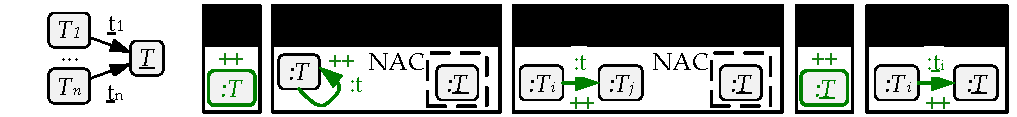
\includegraphics[width=.88\textwidth]{img/software_trans/proof1.pdf}};
\fill (-6.4,0) node[inner sep=1pt] (TG) {$\underline{\TG}=$};
\fill (-3.6,.43) node[inner sep=1pt] (1) {$\textcolor{white}{\code{a}_T}$};
\fill (-2.7,.43) node[inner sep=1pt] (2) {$\textcolor{white}{\code{ar}_t}$};
\fill (.35,.43) node[inner sep=1pt] (3) {$\textcolor{white}{\code{a}_t}$};
\fill (4,.43) node[inner sep=1pt] (4) {$\textcolor{white}{\underline{T}}$};
\fill (4.9,.43) node[inner sep=1pt] (5) {$\textcolor{white}{\underline{t}_i}$};
\end{tikzpicture}
\end{center}
Type graph $\TG'=\TG +_{V_\TG} \underline{\TG},V_\TG=\{T_1,\ldots,T_n\}$ is $\TG$ extended by node $\underline{T}$ and edges $\underline{t}_i$ to $\underline{T}$ from each node $T_i \in \TG$ with inclusion $i_t\colon \TG \to \TG'$.
We define the obvious functor $F\colon \cat{C} \to \cat{C'}$ with $F((G,\type_G)):=(G,i_t \circ \type_G)$ and $F(m):=m$, for all $(G,\type_G) \in \ob_\cat{C}$ and $m \in \morB_\cat{C}$ which is naturally extended to the mapping $\overline{F}(C)$ of sets $C$ of constraints inductively defined by:
\begin{center}
$\overline{F}(\true):=\true$,\\
$\overline{F}(\exists(a\colon P \to C,c)):=\exists(F(a)\colon F(P) \to F(C),\overline{F}(c))$,\\
$\overline{F}(\neg c):=\neg \overline{F}(c)$,\\
$\overline{F}(\wedge_{j \in J}(c_j)):=\wedge_{j \in J}(\overline{F}(c_j))$, and\\
$\overline{F}(\vee_{j \in J}(c_j)):=\vee_{j \in J}(\overline{F}(c_j))$
\end{center}
The mapping $\overline{F}(C)$ is given by $\overline{F}(C):=\cup_{c \in C}(\{\overline{F}(c)\})$.\thispagestyle{plain}
Obviously, for all $G \in \cat{C}$, all sets of constraints $C$ and all $G' \in \cat{C'}$ with inclusions $i_G\colon F(G) \to G'$ and $type_{G'}(e) \in \TG' \setminus i_t(\TG), \forall e \in G' \setminus i_G(F(G))$, it holds that $G \models C \Leftrightarrow G' \models \overline{F}(C)$ $^{(*^3)}$.
For each node $T \in \TG$ there is a plain rule $\code{a}_T\in P$ defined that creates a single node of type $T$.
For each edge $t \in \TG$ with source $T_i$ and target $T_j$ there is a rule $(\code{a}_t,\NAC) \in P$ defined that creates an edge of type $t$ between existing source and target nodes \code{:T_i} and \code{:T_j} but only if there does not already exist a node of type $\underline{T}$.
For each reflexive edge $t \in \TG$ on node $T$ there is a rule $(\code{ar}_t,\NAC) \in P$ defined that creates a reflexive edge of type $t$ on node \code{:T} but only if there does not already exist a node of type $\underline{T}$.
Additionally, there is rule $(\underline{T},\LA(\underline{T},\overline{F}(C))) \in P$ defined that creates a single node of type $\underline{T}$ and for each edge $\underline{t}_i \in \TG'$ from node $T_i$ to $\underline{T}$ there is a rule $(\underline{t}_i,\LA(\underline{t}_i,\overline{F}(C))) \in P$ defined that creates an edge of type $\underline{t}_i$ between nodes \code{:T_i} and \code{:\underline{T}}.
Note that the last rules are only applicable if the application conditions $\LA(\underline{T},\overline{F}(C))$ and $\LA(\underline{t}_i,\overline{F}(C))$ are satisfied, respectively, which are obtained from conditions $C$ as given in \cref{lem:sce-ds-general:trafo_c_ac}.
We assume $\M$-matching for rule applications.
If neglecting the application conditions for rules $\underline{T}$ and $\underline{t}_i$, then $\Lang(\GG)$ contains all graphs in $\cat{C'}$ $^{(*^4)}$.
It remains to show that $C$ is satisfied by all graphs in $\cat{C}$ if and only if $\Lang(C') \subseteq \Lang(\GG)$ holds in $\cat{C'}$.
Then, assuming that the language inclusion problem is decidable would imply that the tautology problem is decidable leading to a contradiction by $(*^2)$.
\begin{itemize}
  \item[``$\Rightarrow$''] We need to show that the tautology of $C$ in $\cat{C}$ implies that $\Lang(\GG)$ contains all graphs in $\cat{C'}$, since, $\Lang(C')$ contains all graphs in $\cat{C'}$.
  By contradiction, assume that there is some $G \in \cat{C'}$ with $G \not\in \Lang(\GG)$.
  Thus by $(*^4)$, there is some $G' \in \cat{C'}$, production $(p\colon L \to R,\LA(p,\overline{F}(C)))\in P$ with $p=\underline{T}$ or $p=\underline{t}_i$ and match $m\colon L \to G'$ such that $m \not\models \LA(p,\overline{F}(C))$.
  By \cref{lem:sce-ds-general:trafo_c_ac}, it follows that $G' \not\models \overline{F}(C)$.
  By definition of $\cat{C},\cat{C'}$ and $F$, there exists $G'' \in \cat{C}$ with inclusion $i_{G''}\colon F(G'') \to G'$ and $\type_{G'}(e) \in \TG'\setminus i_t(\TG),\forall e \in G'\setminus i_{G''}(F(G''))$.
  By $(*^3)$, $G'' \not\models C$.
  \item[``$\Leftarrow$''] We need to show that if $\Lang(\GG)$ contains all graphs in $\cat{C'}$, then $C$ is satisfied by every graph in $\cat{C}$.
  By contradiction, assume that there is some $G \in \cat{C}$ with $G \not\models C$.
  \begin{enumerate}
    \item[\textbf{Case $G=\varnothing$}] We consider a graph $G' \in \cat{C'}$ which consists of a single \code{:\underline{T}} node only.
    By $(*^3)$, $F(G)\not\models \overline{F}(C)$.
    By \cref{lem:sce-ds-general:trafo_c_ac}, for all matches $m\colon L \to F(G)$ from production $\underline{T}\colon L \to R$ it is true that $m \not\models \LA(\underline{T},\overline{F}(C))$.
    Thus, $G' \not\in \Lang(\GG)$, since, $(\underline{T},\LA(\underline{T},\overline{F}(C)))$ is the only rule in $P$ that creates \code{:\underline{T}} nodes.
    \item[\textbf{Case $G\neq\varnothing$}] We consider a graph $G' \in \cat{C'}$ which is $G$ on the $i_t(\TG)$ part and where all nodes \code{:T_i} typed over $i_t(\TG)$ are connected to a single \code{:\underline{T}} node via \code{:\underline{t}_i} edges.
    By the construction of $P$ with NACs for rules $\code{a}_t$ and $\code{ar}_t$ it is guaranteed that rule $(\underline{t}_i,\LA(\underline{t}_i,\overline{F}(C)))$ is the last rule applied via a match $m\colon L \to G''$ to obtain $G'$ with inclusion $i_G\colon F(G) \to G''$ and $\type_{G''}(e) \in \TG'\setminus i_t(\TG), \forall e \in G'' \setminus i_G(F(G))$.
    By $(*^3)$, $G'' \not\models \overline{F}(C)$ and furthermore by \cref{lem:sce-ds-general:trafo_c_ac}, $m \not\models \LA(\underline{t}_i,\overline{F}(C))$.
    Thus, $G' \not\in \Lang(\GG)$.
  \end{enumerate}
  Finally, $\GG$ is non-deleting by construction, $P$ is finite, since, $\TG$ is finite and furthermore, all application conditions in $P$ are finite and in $\M$-normal form by construction, since, $\overline{F}(C)$ preserves the finiteness of set $C$ and the finiteness and $\M$-normal form of each $c_j \in C$.
  Furthermore, transformation $\LA$ leads to finite conditions by the finiteness of set $\overline{F}(C)$ for conjunction $\wedge_{j \in J}$ and the fact that transformation $\text{A}$ preserves the finiteness of each $c_j \in \overline{F}(C)$ by the finiteness of the graphs in $\cat{C'}$ (cf. \cite{DBLP:journals/mscs/HabelP09}).
  As we assume $\M$-matches for rule applications only, all application conditions over $L$ that are not in $\M$-normal form can be transformed into equivalent application conditions over $L$ in $\M$-normal form.
  The construction and proof is identical to Def. 5 and the proof of Fact 6 in \cite{DBLP:journals/mscs/HabelP09}.
  $C'$ is trivially finite and in $\M$-normal form.
\end{itemize}
\qed

\section{Proof of \cref{sec-dc-verification,th:sec-dc-verification:term_dc}}
\label{sec-proofs:th:sec-dc-verification:term_dc}
The termination of the verification of both conditions is considered separately implying further the termination of the verification of domain completeness up to the given upper bound.
\begin{enumerate}
  \item For $C$-extension completeness we conclude as follows.
  The set of atoms that are typed over the type graph is finite up to isomorphism, since, the type graph is finite.
  Due to the fact that upper bound $G_u$ is finite, the set of graphs $Graphs_{G_u}=\{G \mid G \in \Lang(\TG),\exists G \to G_u \in \M\}$ is finite up to isomorphism as well as its computation terminates and therefore, also the set of graphs $\Lang(C)_{G_u} \subseteq Graphs_{G_u}$ is finite up to isomorphism.
  The check whether $G \in Graphs_{G_u}$ is also in $\Lang(C)_{G_u}$, i.e., $G \in \Lang(C)_{G_u}$, terminates in each case, since, $G$ is finite by finite upper bound $G_u$, $C$ is finite and moreover, each constraint $c \in \C$ is finite with a finite number of nestings.
  Therefore, the set of effective atoms $EAtoms(C)$ is finite up to isomorphism and furthermore, the identification of their effectiveness w.r.t. $\Lang(C)_{G_u}$ terminates, since, for each atom $a$ we can iterate over finite $\Lang(C)_{G_u}$ in order to find $G \in \Lang(C)_{G_u}$ with inclusion $a \to G \in \M$.
  The inclusion checking terminates in each case, since, $G$ is finite by finite upper bound $G_u$.
  Note that if a graph $G$ is significant w.r.t. $\Lang(C)_{G_u}$ ($\exists G \to H \in \M,H \in \Lang(C)_{G_u}$), then $G$ is finite, since, all graphs in $\Lang(C)_{G_u}$ are finite by finite upper bound $G_u$ and so their $\M$-subobjects $G$.
  Concerning the extensions $Extensions(a,C)$ of each effective atom $a$, all graphs in $Extensions(a,C)$ are significant w.r.t. $\Lang(C)_{G_u}$ by construction \cref{def:C-extension} and therefore also finite.
  Note that if a graph $G$ is significant w.r.t. $\Lang(C)_{G_u}$ ($\exists i_1\colon G \to H \in \M,H \in \Lang(C)_{G_u}$ with $i_2 \colon H \to G_u \in \M$ by definition of $\Lang(C)_{G_u}$), then $G \in Graphs_{G_u}$, since, $\exists i_2 \circ i_1\colon G \to G_u \in \M$ by $\M$-composition.
  Thus, $Graphs_{G_u}$ contains all graphs that are significant w.r.t. $\Lang(C)_{G_u}$.
  Therefore, the fact that $Extensions(a,C)$ only contains graphs that are significant w.r.t. $\Lang(C)_{G_u}$ and that set $Graphs_{G_u}$ is finite implies that each extension $E \in Extensions(a,C)$ is a finite set of graphs up to isomorphism.
  Note that the power set $\mathcal{P}(Graphs_{G_u})$ of the set $Graphs_{G_u}$ of significant graphs w.r.t. $\Lang(C)_{G_u}$ is finite by the finiteness of $Graphs_{G_u}$.
  Thus, as $Extensions(a,C)$ only contains significant graphs w.r.t. $\Lang(C)_{G_u}$, $\mathcal{P}(Graphs_{G_u})$ represents all possible extensions and therefore, $Extensions(a,C)$ is a finite set of extensions up to isomorphism.
  Finally, we can iterate over all effective atoms $a \in EAtoms(C)$, iterate over all extensions $E \in Extensions(a,C)$ and check for each graph $G \in E$ whether $G$ can be created via grammar $\GG$ from the empty start graph.
  The check terminates for each $G$, since, the set of rules of $\GG$ is finite and each rule is non-deleting and non-trivial, i.e., the number of branches of direct transformation steps are finite at each step and the graph is extended by at least one element (node, edge or attribute) after each step and therefore, for each branch, we stop if the size of the graph is bigger than finite $G$.
  The verification of the satisfaction of application conditions of rules in each step terminates, since, the conditions are finite with a finite number of nestings.
  Therefore, the verification of $C$-extension completeness terminates.
  
  Note that construction \cref{def:C-extension} for constructing the $Extensions(a,C)$ of each effective atom $a$ terminates as shown below and therefore, the construction can be directly used as algorithm to compute the extensions.\thispagestyle{plain}
  At each extension via $extend(G_E,\ac_P,m)$, the number of overlappings of $G_E$ and $C$ via $P'$ in $extend(G_E,f,m)$ is finite up to isomorphism in each case, since, all conclusions $C$ of all constraints are finite graphs.
  Analogously to the identification of the effectiveness of atoms w.r.t. $\Lang(C)_{G_u}$, the identification of the significance of graphs w.r.t. $\Lang(C)_{G_u}$ terminates.
  Furthermore, the constraints $\ac_P$ are finite with a finite number of nestings leading to a finite number of iterations via $extend(G_E,\ac_P,m)$, i.e., each extension via $extend(G_E,\ac_P,m)$ terminates.
  Moreover, the set of constraints $C$ is finite, the premise of each constraint is a finite graph and therefore, the set of instances $\Inst(C)$ of $C$ is finite up to isomorphism.
  Therefore, there are finitely many extensions via $extend(G_E,\ac_P,m)$ for each graph of an extension, which is again a finite set of graphs as shown above.
  Therefore, we can step-wise compute extensions and stop a branch if it yields an extension that was already computed.
  The procedure terminates, since, there are only finitely many $Extensions(a,C)$ as shown above.
  \item For $C$-conflict-freeness of marking rules we conclude as follows.
  Note that $Graphs_{G_u}$ is finite up to isomorphism and the set of all graphs that are significant w.r.t. $\Lang(C)_{G_u}$ as shown above.
  Therefore, we can iterate over all graphs $O \in Graphs_{G_u}$ in order to collect all critical pairs with conflict graph $O$ that are significant w.r.t. $\Lang(C)_{G_u}$.
  The procedure terminates, since, the set of rules of $\GG$ and therefore the set of all their combinations is finite, all graphs are finite for matching and all application conditions are finite with a finite number of nestings such that verifying their satisfaction terminates.
  Finally, we can iterate over the finite set of critical pairs that are significant w.r.t. $\Lang(C)_{G_u}$ and check if each pair is strictly confluent.
  The confluence analysis terminates in each case, since, we have finitely many non-trivial marking rules where each direct transformation step via marking rules updates at least one marking attribute from $\False$ to $\True$ until there is no applicable marking rule anymore or all marking attributes in finite $O$ are set to $\True$.
  \qed
\end{enumerate}

\section{Proof of \cref{sec-dc-verification,lem:equivalence-marking-emptySG}}
\label{sec-proofs:lem:equivalence-marking-emptySG}
The main part of this result has been shown already in \cite{heocdx11} for the more complex setting of triple graphs based on the fully formalised
concepts for translation attributes~\cite{Hermann:2010:EAE:1866272.1866277}.
Hence, we reuse that equivalence result for triple sequences for the present case.
First, note that each graph $H$ can be extended to a triple graph 
$\I(H)=(H \transB{\varnothing} \varnothing \trans{\varnothing} \varnothing)$ with empty correspondence and target component
via inclusion functor $\I$.
Moreover, each rule (morphism) $(r\colon L\to R) \in P$ can be extended to a triple rule (morphism) 
$\I(r)=(r,\varnothing,\varnothing)\colon \I(L) \to \I(R)$ 
with empty correspondence and target component via inclusion functor $\I$.
Given a set of rules $P$, then $\I(P) = \{\I(p) \mid p \in P\}$.
Analogously, each match morphism can be extended and each marking rule $m(p)=(L \xhookleftarrow{l} K \xhookrightarrow{r} R)$ can be extended to $\I(m(p))=(\I(L) \xhookleftarrow{\I(l)} \I(K) \xhookrightarrow{\I(r)} \I(R))$.
We derive the equivalence as follows:
\\
\begin{tabular}{lp{0.95\textwidth}}
& $\exists$ transformation sequence	$(1)=(G \oplus \Att_G^\False \Trans{*} G \oplus \Att_{G_k}^\True \oplus \Att_{G \setminus G_k}^\False)$ via marking rules $m(\GG)$ with intermediate steps $G'_i \Trans{(m'_i,m(p_i))} G'_{i+1}$ %$, m(p_i)=(L_i \xhookleftarrow{} K_i \xhookrightarrow{} R_i)$ and $\quotient{m_i}{L_i^{\False}}$ is type strict
\\
$\Leftrightarrow$
& $\exists$ transformation sequence $\I(G) \oplus \Att_{\I(G)}^\False \Trans{*} \I(G) \oplus \Att_{\I(G_k)}^\True \oplus \Att_{\I(G) \setminus \I(G_k)}^\False$ via marking rules $\I(m(\GG))$ %(extension $\I$ adds empty source and target components)
%with intermediate steps $\I(G'_i) \Trans{\I(m_i),\I(m(p_i))} \I(G'_{i+1}), \I(m(p_i))=(\I(L_i) \xhookleftarrow{} \I(K_i) \xhookrightarrow{} \I(R_i))$ and $\quotient{\I(m_i)^S}{\I(L_i)^{S,\False}}$ is type strict
\\
$\Leftrightarrow$
&
	$\exists$ a transformation sequence $\I(\varnothing) \Trans{*} \I(G_k)$ via $\I(P)$ with injective embedding $\I(f)\colon \I(G_k) \to \I(G)$ by \cref{sec-msynch-tgg,fact:sec-msynch-tgg:equ_tr_cc}
\\
$\Leftrightarrow$
&
	$\exists$ a transformation sequence $(2)=\varnothing \Trans{*} G_k$ via $P$ with injective embedding $f\colon G_k \to G$ and with intermediate steps $G_i \Trans{(m_i,p_i)} G_{i+1}$ (by restriction to the source component).
\end{tabular}
The correspondence of rules between the intermediate steps $G'_i \Trans{(m'_i,m(p_i))} G'_{i+1}$ in sequence $(1)$ and $G_i \Trans{(m_i,p_i)} G_{i+1}$ in sequence $(2)$ follows from Lemma 1 in~\cite{heocdx11} and for the equivalence of triple steps and corresponding marking (consistency creating) steps and its application in the proof for \cref{sec-msynch-tgg,fact:sec-msynch-tgg:equ_tr_cc}.
\qed

\section{Proof of \cref{sec-dc-verification,lem:equivalence-marking}}
\label{sec-proofs:lem:equivalence-marking}
Let $\GG=(S,P)$ be a graph grammar with a set $P$ of non-deleting rules and $m(\GG)$ be the set of derived marking rules of $\GG$. 
Let $G$ be a graph and let $\GG'$ be a graph grammar given by $\GG'=(\varnothing, P \cup \{p_{S}=(\varnothing \to S)\})$.
Then, there is the transformation step $\varnothing \Trans{p_{S}} S$ via $\GG'$ and there is the transformation step $G \oplus \Att_G^\False = G \oplus \Att_{S}^\False \oplus \Att_{G\setminus S}^\False \Trans{m(p_{S})} G \oplus \Att_{S}^\True \oplus \Att_{G\setminus S}^\False$ via $m(\GG')$.
Using \cref{lem:equivalence-marking-emptySG}, this implies that the following are equivalent.
\begin{itemize}
	\item $\exists$ a transformation sequence $G \oplus \Att_G^\False = G \oplus \Att_{S}^\False \oplus \Att_{G\setminus S}^\False \Trans{m(p_{S})} G \oplus \Att_{S}^\True \oplus \Att_{G\setminus S}^\False \Trans{*} G \oplus \Att_G^\True$ via marking rules $m(\GG)$.% with intermediate steps $G'_i \Trans{m(p_i)} G'_{i+1}$, where $p_i \in P$ for $i>1, m(p_i)=(L_i \xhookleftarrow{} K_i \xhookrightarrow{} R_i)$ and $\quotient{m_i}{L_i^{\False}}$ is type strict
	\item $\exists$ a transformation sequence $\varnothing \Trans{p_{S}} S \Trans{*} G$	via $P$.% with intermediate steps $G_i \Trans{p_i} G_{i+1}$, where $p_i \in P$ for $i>1$.
\end{itemize}
Since the first step in any of the two sequences is always possible, we derive the result of the lemma.
\qed

\section{Proof of \cref{sec-dc-verification,lemma:closure-c-ext}}
\label{sec-proofs:lemma:closure-c-ext}
Let $G \in \Lang(C), a \in A \in Atoms(G)$ with embedding $e\colon a \to G \in \M$ and $E_n \in Extensions(a,C)$.
We assume that $E_n$ is derived by extension sequence $(E_j \Trans{extend(a_E^j,c_j,m_j)} E_{j+1})_{j \in \{0,\ldots,n-1\}}$ with $E_0=\{a\}, \forall j \in \{0,\ldots,n-1\}.a_E^j \in E_j, (f_j \in \E,\morO,c_j) \in \Inst(C), c_j \equiv \vee_{i \in I} \exists (\ac_i\colon P'_j \to C'_i, \ac_{C'_i})$ and $m_j\colon P'_j \to a_E^j \in \M$ according to \cref{def:C-extension}.
In the following we show that there is $a_E^n \in E_n$  with morphisms $e_1\colon a \to a_E^n \in \M$ and $e_2\colon a_E^n \to G \in \M$ with $e=e_2 \circ e_1$ by induction over the extension sequence.
For each step $j$ of the sequence we conclude as follows.
For graph $a_E^j$ with embedding $e_j\colon a_E^j \to G \in \M$, we derive extended graph $a_E^{j+1} \in E_{j+1}$ with embeddings $c_j\colon a_E^j \to a_E^{j+1} \in \M$ and $e'_j\colon a_E^{j+1} \to G \in \M$ and with $e_j=e'_j \circ c_j$ as follows.\thispagestyle{plain}
\begin{center}
% $
% \SelectTips{cm}{}
%      \xymatrix@R5ex@C10ex{
%      P \ar@{->}[d]|{f \in \E} \ar@/_14ex/[ddddr]|{p \in \morO} & & & & \\
%      P' \ar@{.>}[r]|{a} \ar@{->}[ddr]|{m \in \M} \ar@/_4ex/[dddr]|{p' \in \M} \ar@/^5ex/[rrrr]|{\ac_i \in \M} & P'' \ar@{.>}[rrr]|{b} \ar@{.>}[dd]|{c} & & & C_i' \ar@{.>}[ddl]|{c'} \ar@/^10ex/[dddlll]|{q' \in \M} \\
%      && (1) &&\\
%      & a_E^i \ar@{->}[d]|{e \in \M} \ar@{.>}[rr]|{b'} & & a_E^{i+1} \ar@{.>}[dll]|{e' \in \M} & \\
%      & G & & &
%      }
% $
\begin{tikzpicture}[]
\fill (.5,0) node[inner sep=1pt] (P) {$P$};
\fill (2,-1) node[inner sep=1pt] (P') {$P'_j$};
\fill (5,-1) node[inner sep=1pt] (P'') {$P''_j$};
\fill (5,-2.5) node[inner sep=1pt] (aei) {$a_E^j$};
\fill (5,-3.5) node[inner sep=1pt] (G) {$G$};
\fill (8,-2.5) node[inner sep=1pt] (aei2) {$a_E^{j+1}$};
\fill (11,-1) node[inner sep=1pt] (C'i) {$C'_i$};
\fill (6.5,-1.75) node[inner sep=1pt] (PO) {(1)};
\fill (3.5,-1.35) node[inner sep=1pt] (EQ1) {(2)};
\fill (6.5,-.5) node[inner sep=1pt] (EQ2) {(3)};
\fill (6,-2.8) node[inner sep=1pt] (EQ3) {(4)};
\fill (8.5,-2.8) node[inner sep=1pt] (EQ4) {(5)};
%
\fill (11.6,-1) node [isosceles triangle, rotate=180, fill=gray!25,draw,minimum width=0.4cm, inner sep=1pt] (t) {};
\fill (12.1,-1) node[inner sep=1pt] {$\ac_{C'_i}$};
%
{
\pgfsetarrows{*-latex}
\draw (P) edge[bend right=45] node[left,inner sep=5pt]{$\scriptstyle{p_j \in \morO}$} (G);

\pgfsetarrows{*->>}
\draw (P) -> node[above,inner sep=1pt,xshift=2ex]{$\scriptstyle{f_j \in \E,\morO}$} (P');

\pgfsetarrows{right hook-latex}
\draw (P') edge[bend left=20] node[above,inner sep=1pt]{$\scriptstyle{ac_i \in \M}$} (C'i);
\draw (P') -> node[right,xshift=.8ex,yshift=0.2ex]{$\scriptstyle{m_j \in \M}$} (aei);
\draw (aei) -> node[right,inner sep=1pt]{$\scriptstyle{e_j \in \M}$} (G);

\pgfsetarrows{left hook-latex}
\draw (P') -> node[left,inner sep=4pt]{$\scriptstyle{p'_j \in \M}$} (G);
\draw (C'i) edge[bend left=35] node[right,xshift=6ex,yshift=3ex]{$\scriptstyle{q'_j \in \M}$} (G);

\pgfsetarrows{-latex}
\draw[dotted] (P'') -> node[above,inner sep=1pt]{$\scriptstyle{\ac'_i}$} (C'i);
\draw[dotted] (P') -> node[above,inner sep=1pt]{$\scriptstyle{a_i}$} (P'');
\draw[dotted] (P'') -> node[right,inner sep=1pt]{$\scriptstyle{m'_j}$} (aei);
\draw[dotted] (C'i) -> node[right,inner sep=4pt]{$\scriptstyle{b_j}$} (aei2);
\draw[dotted] (aei) -> node[above,inner sep=1pt]{$\scriptstyle{c_j}$} (aei2);
\draw[dotted] (aei2) -> node[right,inner sep=4pt, yshift=-.5ex]{$\scriptstyle{e'_j}$} (G); 
%
}
\end{tikzpicture}
\end{center}
Let match $p_j\colon P \to G=p'_j \circ f_j$ with $p'_j=e_j \circ m_j$.
By \cref{sec-gt-M-adh,rem:sec-gt-M-adh:agraphs_atgi} with $f_j \in \morO$ and $m_j,e_j \in \M$, $p_j \in \morO$ and $p'_j \in \M$ by $\M$-composition.
$G \in \Lang(C)$ and \cref{sec-gt-gc,rem:sec-gc-gc:init_gen_sat_ac_schema} imply that $p'_j \models c_j$.
Therefore, $p'_j \models \exists(\ac_i, \ac_{C'_i})$ for some $i \in I$, i.e., there exists morphism $q'_j\colon C_i' \to G \in \M$ with $q'_j \circ \ac_i=p'_j$.
We construct pullback $(\ac'_i,m'_j)$ over morphisms $(e_j,q'_j)$ with $e_j \circ m'_j=q'_j \circ \ac'_i$ $^{(*^1)}$.
By $e_j,q'_j \in \M$ and $\M$-morphisms are closed under pullbacks, it follows that $\ac'_i,m'_j \in \M$. 
By the universal pullback property with $e_j \circ m_j=p'=q'_j \circ \ac_i$ we obtain unique morphism $a_i\colon P'_j \to P''_j$ with commuting (2) and (3).
Furthermore, $\ac_i,\ac'_i \in \M$ and $\M$-decomposition imply that $a_i \in \M$.
We construct pushout (1) over morphisms $(m'_j,\ac'_i)$.
Since $\ac'_i,m'_j \in M$ and $\M$-morphisms are closed under pushouts, it follows that $b_j,c_j \in \M$.
By $(*^1)$ and the universal pushout property we obtain unique morphism $e'_j\colon a_E^{j+1} \to G$ with commuting (4) and (5).
By effective pushouts it follows that $e'_j \in \M$.
Thus, there is an embedding $e'_j$ from extended graph $a_E^{j+1}$ to $G$, i.e., by assumption $G \in \Lang(C)$ it follows that $a_E^{j+1}$ is significant w.r.t. $\Lang(C)$ implying further that $a_E^{j+1}$ is also not $C$-inconsistent by \cref{rem:sec-gc-verification}.
We can conclude recursively for nestings $\ac_{C'_i}$ of condition $c_j$.
By construction \cref{def:C-extension} it follows that $(b_j,a_E^{j+1}) \in extend(a_E^j,c_j,m_j)$.
Therefore, for an extension step $E_j \Trans{extend(a_E^j,c_j,m_j)} E_{j+1}$ with graph $a_E^j \in E_j$ and embedding $e_j\colon a_E^j \to G \in \M$, it holds that there exists a graph $a_E^{j+1} \in E_{j+1}$ with embeddings $c_j\colon a_E^j \to a_E^{j+1} \in \M$ and $e'_j\colon a_E^{j+1} \to G \in \M$ and with $e_j=e'_j \circ c_j$.
By induction over the steps $s_j$ of extension sequence $(s_j\colon E_j \Trans{extend(a_E^j,c_j,\_)} E_{j+1})_{j \in \{0,\ldots,n-1\}}$, we obtain the desired result, that extension $E_n$ contains a graph $a_E^n$ with morphisms $e_1\colon a \to a_E^n \in \M$ and $e_2\colon a_E^n \to G \in \M$ and with $e=e_2 \circ e_1$.
\textbf{Basis.} For $n=1$, we have extension step $s_0\colon E_0=\{a\} \Trans{extend(a,c_0,\_)} E_1$ with embedding $e\colon a \to G \in \M$ for $a \in A \in Atoms(G)$.
By using the result from above, there exists graph $a_E^1 \in E_1$ with embeddings $e_1\colon a \to a_E^1 \in \M$ and $e_2\colon a_E^1 \to G \in \M$ and with $e=e_2 \circ e_1$.
\textbf{Hypothesis.} There is an $n \in \mathbb{N}$ and extension sequence $(s_j\colon E_j \Trans{extend(a_E^j,c_j,\_)} E_{j+1})_{j \in \{0,\ldots,n-1\}}$ with $E_0=\{a\}, e\colon a \to G \in \M, \forall j \in \{0,\ldots,n-1\}.a_E^j \in E_j,(\_,c_j) \in \Inst(C)$ such that there exists a graph $a_E^n \in E_n$ with embeddings $e_1\colon a \to a_E^n \in \M$ and $e_2\colon a_E^n \to G \in \M$ and with $e=e_2 \circ e_1$.
\textbf{Step.} For $n+1$, we focus on the last step $s_n\colon E_n \Trans{extend(a_E^n,c_n,\_)} E_{n+1}$ of the extension sequence.
\begin{description}
\item[Case (a)] Let $a_E^n \in E_n$ be a graph with embeddings $e'_1\colon a \to a_E^n \in \M$ and $e'_2\colon a_E^n \to G \in \M$ and with $e=e'_2 \circ e'_1$, then we can apply the result from above for step $s_n$ and obtain graph $a_E^{n+1} \in E_{n+1}$ with embeddings $a \trans{e'_1} a_E^n \trans{e_1} a_E^{n+1} \in \M$ (by $\M$-composition) and $e_2\colon a_E^{n+1} \to G \in \M$ and with $e'_2=e_2 \circ e_1$, i.e., $e'_2 \circ e'_1=e_2 \circ e_1 \circ e'_1 \Rightarrow e=e_2 \circ e_1 \circ e'_1$. 
\item[Case (b)] Let $a_E^n \in E_n$ be a graph without the embeddings from Case (a), then there exists another graph ${a'}_E^n \in E_n$ with embeddings $e_1\colon a \to {a'}_E^n \in \M$ and $e_2\colon {a'}_E^n \to G \in \M$ and with $e=e_2 \circ e_1$ by induction hypothesis.
By \cref{def:C-extension}, it holds that ${a'}_E^n \in E_{n+1}$, since, graph ${a'}_E^n$ is not extended by step $s_n$.
\qed
\end{description}

\section{Proof of \cref{sec-dc-verification,lem:union-ext-atoms}}
\label{sec-proofs:lem:union-ext-atoms}
Let $A=(a_i)_{i \in \{1,\ldots,n\}} \in Atoms(G)$ be the atoms of graph $G \in \Lang(C)$ which generally satisfies the set of constraints $C$ with induced morphisms $(e_i\colon a_i \to G \in \M)_{i \in \{1,\ldots,n\}}$ by \cref{lemma:union-atoms}.
Let $f_E \in SELECT_E(A,C)$ be a function that selects a $C$-extension $E_i \in Extensions(a_i,C)$ for each atom $a_i \in A$.
By \cref{lemma:closure-c-ext}, it follows that each $C$-extension $E_i$ contains a graph $a_E^i \in E_i$ with morphisms $e^i_1\colon a_i \to a_E^i \in \M$ and $e^i_2\colon a_E^i \to G \in \M$ and with $e_i=e^i_2 \circ e^i_1$.
Therefore, we can define a function $f_{a_E} \in SELECT_{a_E}(A,C,f_E)$ such that $\forall a_i \in A.f_{a_E}(a_i)=a_E^i$ with morphisms $e^i_1\colon a_i \to f_{a_E}(a_i) \in \M$ and $e^i_2\colon f_{a_E}(a_i) \to G \in \M$ and with $e_i=e^i_2 \circ e^i_1$.
It remains to show that there exists the corresponding sequence of pushouts $(PO^E_k +_{G^E_k} f_{a_E}(a_{k+1}) = PO^E_{k+1})_{k \in \{1,\ldots,n-1\}}$ with pushout objects $PO^E_{k+1}$, $PO^E_1=f_{a_E}(a_1)$ and $PO^E_n=G$.
By induction over the list of atoms $(a_i)_{i \in \{1,\ldots,n\}}$ we conclude as follows.
For $n=1$ the assumption holds trivially.
\textbf{Basis.} For $n=2$ we focus on the diagram below (right).
By \cref{lemma:union-atoms}, there exists pushout $(f'_{n-1} \in \M,e_n \in \M)$ over $(g_{n-1} \in \M,f_{n-1} \in \M)$ with $PO_{n-1}=a_{n-1}, PO_n=G$ and $f'_{n-1}=e_{n-1}$.
Furthermore, let $PO^E_{n-1}=f_{a_E}(a_{n-1}), \ol{e}^{n-1}_1=e^{n-1}_1 \in \M$ and $\ol{e}^{n-1}_2=e^{n-1}_2 \in \M$ such that $(3)$ commutes.
Analogously, commuting $(4)$ is given with $e^n_1,e^n_2 \in \M$.
We can construct pullback $(1)$ by $\ol{e}^{n-1}_2 \in \M$ with $G^E_{n-1} \to f_{a_E}(a_n), G^E_{n-1} \to PO^E_{n-1} \in \M$ by $\M$-morphisms are closed under pullbacks.
Analogously, we can construct pullback $(2)$ with $G'_{n-1} \to a_n \in \M$.
By pullback composition, also $(1)+(2)$ is a pullback with induced unique morphism $G_{n-1} \to G'_{n-1}$ and commuting $(5)$ and $(6)$ by universal pullback property.
By $\M$-pushout-pullback decomposition with the outer pushout diagram, commuting $(3),(4)$ and $(6)$, pullback $(1)+(2)$, and $\ol{e}^{n-1}_2,g_{n-1} \in \M$, it follows that $(1)+(2)$ is a pushout.
Again by $\M$-pushout-pullback decomposition with pushout $(1)+(2)$, pullback $(1)$, and $G'_{n-1} \to a_n,e^n_2 \in \M$, it follows that $(1)$ is the requested pushout with $PO^E_n=PO_n=G$. \\
\\ For $n=3$ we focus on the diagram below (left) with $k=1$.
By \cref{lemma:union-atoms}, there exists pushout $(7)$ with $PO_1=a_1$ and induced morphisms $e_1\colon a_1 \trans{f'_1} PO_2 \trans{f'_2 \in \M} G \in \M,e_2\colon a_2 \trans{g'_1} PO_2 \trans{f'_2 \in \M} G \in \M$.
Furthermore, let $PO^E_1=f_{a_E}(a_1)$ with $\ol{e}^1_1=e^1_1 \in \M$ and $\ol{e}^1_2=e^1_2 \in \M$ implying further that $(7a)$ and $(7b)$ commute.
We construct effective pushout $(8)$ over $(\ol{e}^1_2,e^2_2)$ with all morphisms in $\M$ by $\M$ is closed under pushouts and pullbacks, pullback $(8)+(8a)+(8b)$ and induced morphism $\ol{e}^2_2 \in \M$ such that $(8a)$ and $(8b)$ commute.
By the universal pushout property of $(7)$ with $f'_1 \circ g_1 \stackrel{(7)}{=} g'_1 \circ f_1$ $\Rightarrow f'_2 \circ f'_1 \circ g_1=f'_2 \circ g'_1 \circ f_1$ there is a unique morphism $PO_2 \to G=f'_2 \in \M$ such that $(7a)+(8a)+(8c)$ and $(7b)+(8b)+(8d)$ commute.
Again by the universal pushout property of $(7)$ with $f'_2 \circ f'_1 \circ g_1=f'_2 \circ g'_1 \circ f_1$ $\Leftrightarrow e_1 \circ g_1=e_2 \circ f_1$ $\stackrel{(7a),(7b)}{\Rightarrow} \ol{e}^1_2 \circ \ol{e}^1_1 \circ g_1=e^2_2 \circ e^2_1 \circ f_1$ $\stackrel{(8a),(8b)}{\Rightarrow}$ $\ol{e}^{2}_2 \circ a_1 \circ \ol{e}^1_1 \circ g_1=\ol{e}^{2}_2 \circ b_1 \circ \ol{e}^2_1 \circ f_1$ $\stackrel{\ol{e}^2_2\text{ is mono}}{\Rightarrow}$ $a_1 \circ \ol{e}^1_1 \circ g_1=b_1 \circ \ol{e}^2_1 \circ f_1$, there is morphism $\ol{e}^2_1$ such that $(8c)$ and $(8d)$ commute.
Thus, for $\ol{e}^2_2 \circ \ol{e}^2_1$, $(7a)+(8a)+(8c)$ and $(7b)+(8b)+(8d)$ commute, i.e., the uniqueness of morphism $f'_2 \in \M$ implies that $f'_2=\ol{e}^2_2 \circ \ol{e}^2_1$.
By $\M$-decomposition with $\ol{e}^2_2 \in \M$ it follows that $\ol{e}^2_1 \in \M$.
By \cref{lemma:union-atoms}, there exists pushout $(f'_2 \in \M,e_3 \in \M)=(1)+\ldots+(6)$ over $(g_{n-1} \in \M,f_{n-1} \in \M)$ in the diagram below (right) with $PO_3=G$, $\ol{e}^2_1,\ol{e}^2_2,f'_2 \in \M$ from above such that $(3)$ commutes.
Analogously to base case with $n=2$, we obtain puhsout $(1)$ leading to the requested sequence of pushouts $(8)$ and $(1)$ with pushout object $PO^E_3=G$.
\begin{center}
\begin{tikzpicture}[]
\fill (0,0) node[inner sep=1pt] (POnm1) {$PO_{n-1}$};
\fill (6,0) node[inner sep=1pt] (an) {$a_n$};
\fill (3,0) node[inner sep=1pt] (GEnm1) {$G^E_{n-1}$};
\fill (3,-3) node[inner sep=1pt] (Gnm1) {$G_{n-1}$};
\fill (3,3) node[inner sep=1pt] (POn) {$PO^E_n=PO_n=G$};
\fill (1.5,1.5) node[inner sep=1pt] (POEnm1) {$PO^E_{n-1}$};
\fill (4.5,1.5) node[inner sep=1pt] (fae) {$f_{a_E}(a_n)$};
\fill (4.5,-1.5) node[inner sep=1pt] (G'nm1) {$G'_{n-1}$};
%
\fill (3,1.5) node[inner sep=1pt] (1) {$(1)$};
\fill (4.5,0) node[inner sep=1pt] (2) {$(2)$};
\fill (1,2.25) node[inner sep=1pt] (3) {$(3)$};
\fill (5,2.25) node[inner sep=1pt] (4) {$(4)$};
\fill (2,-1) node[inner sep=1pt] (5) {$(5)$};
\fill (4.5,-2.25) node[inner sep=1pt] (6) {$(6)$};
%
\fill (-4.5,-3) node[inner sep=1pt] (2Gk) {$G_k$};
\fill (-7.5,-2) node[inner sep=1pt] (2POk) {$PO_k$};
\fill (-1.5,-2) node[inner sep=1pt] (2akp1) {$a_{k+1}$};
\fill (-4.5,3) node[inner sep=1pt] (2G) {$G$};
\fill (-4.5,-1) node[inner sep=1pt] (2POkp1) {$PO_{k+1}$};
\fill (-6.5,1) node[inner sep=1pt] (2POEk) {$PO_k^E$};
\fill (-2.5,1) node[inner sep=1pt] (2faE) {$f_{a_E}(a_{k+1})$};
\fill (-4.5,2) node[inner sep=1pt] (2POEkp1) {$PO^E_{k+1}$};
\fill (-4.5,0) node[inner sep=1pt] (2GEk) {$G^E_k$};
%
\fill (-4.5,-2) node[inner sep=1pt] (7) {$(7)$};
\fill (-4.5,1) node[inner sep=1pt] (8) {$(8)$};
\fill (-7.15,.5) node[inner sep=1pt] (7a) {$\scriptsize{(7a)}$};
\fill (-1.85,.5) node[inner sep=1pt] (7b) {$\scriptsize{(7b)}$};
\fill (-5.35,2) node[inner sep=1pt] (8a) {$\scriptsize{(8a)}$};
\fill (-3.65,2) node[inner sep=1pt] (8b) {$\scriptsize{(8b)}$};
\fill (-5.75,-.5) node[inner sep=1pt] (8c) {$\scriptsize{(8c)}$};
\fill (-3.25,-.5) node[inner sep=1pt] (8d) {$\scriptsize{(8d)}$};
%
{
\pgfsetarrows{*-latex}
\pgfsetarrows{*->>}
\pgfsetarrows{right hook-latex}
\pgfsetarrows{left hook-latex}
\pgfsetarrows{-latex}
\draw (Gnm1) edge[bend left=55] node[fill=white,inner sep=5pt]{$\scriptstyle{g_{n-1}}$} (POnm1);
\draw (Gnm1) edge[bend right=55] node[fill=white,inner sep=5pt]{$\scriptstyle{f_{n-1}}$} (an);
\draw (POnm1) edge[bend left=55] node[fill=white,inner sep=5pt]{$\scriptstyle{f'_{n-1}}$} (POn);
\draw (an) edge[bend right=55] node[fill=white,inner sep=5pt]{$\scriptstyle{e_n}$} (POn);
\draw (POnm1) edge[] node[fill=white,inner sep=5pt]{$\scriptstyle{\ol{e}^{n-1}_1}$} (POEnm1);
\draw (POEnm1) edge[] node[fill=white,inner sep=5pt]{$\scriptstyle{\ol{e}^{n-1}_2}$} (POn);
\draw (an) edge[] node[fill=white,inner sep=5pt]{$\scriptstyle{e^n_1}$} (fae);
\draw (fae) edge[] node[fill=white,inner sep=5pt]{$\scriptstyle{e^n_2}$} (POn);
\draw (GEnm1) edge[dotted] node[inner sep=5pt]{$\scriptstyle{}$} (POEnm1);
\draw (GEnm1) edge[dotted] node[inner sep=5pt]{$\scriptstyle{}$} (fae);
\draw (G'nm1) edge[dotted] node[inner sep=5pt]{$\scriptstyle{}$} (GEnm1);
\draw (G'nm1) edge[dotted] node[inner sep=5pt]{$\scriptstyle{}$} (an);
\draw (Gnm1) edge[dotted] node[inner sep=5pt]{$\scriptstyle{}$} (G'nm1);
%
\draw (2Gk) edge[] node[fill=white,inner sep=5pt]{$\scriptstyle{g_k}$} (2POk);
\draw (2Gk) edge[] node[fill=white,inner sep=5pt]{$\scriptstyle{f_k}$} (2akp1);
\draw (2POk) edge[] node[fill=white,inner sep=5pt]{$\scriptstyle{f'_k}$} (2POkp1);
\draw (2akp1) edge[] node[fill=white,inner sep=5pt]{$\scriptstyle{g'_k}$} (2POkp1);
\draw (2POk) edge[bend left=55] node[fill=white,inner sep=5pt,yshift=1cm]{$\scriptstyle{f'_{n-1} \circ \ldots \circ f'_k}$} (2G);
\draw (2akp1) edge[bend right=55] node[fill=white,inner sep=5pt,yshift=1cm]{$\scriptstyle{f'_{n-1} \circ \ldots \circ f'_{k+1} \circ g'_k}$} (2G);
\draw (2POk) edge[] node[fill=white,inner sep=5pt]{$\scriptstyle{\ol{e}^k_1}$} (2POEk);
\draw (2POEk) edge[bend left=40] node[right,inner sep=5pt]{$\scriptstyle{\ol{e}^k_2}$} (2G);
\draw (2akp1) edge[] node[fill=white,inner sep=5pt]{$\scriptstyle{e^{k+1}_1}$} (2faE);
\draw (2faE) edge[bend right=40] node[left,inner sep=5pt]{$\scriptstyle{e^{k+1}_2}$} (2G);
\draw (2GEk) edge[dotted] node[inner sep=5pt]{$\scriptstyle{}$} (2POEk);
\draw (2GEk) edge[dotted] node[inner sep=5pt]{$\scriptstyle{}$} (2faE);
\draw (2POEk) edge[dotted] node[inner sep=5pt]{$\scriptstyle{}$} (2POEkp1);
\draw (2faE) edge[dotted] node[inner sep=5pt]{$\scriptstyle{}$} (2POEkp1);
\draw (2POEkp1) edge[dotted] node[inner sep=5pt,yshift=-.15cm]{$\scriptstyle{\ol{e}^{k+1}_2}$} (2G);
\draw (2POkp1) edge[dotted] node[right,inner sep=5pt,yshift=-1cm]{$\scriptstyle{\ol{e}^{k+1}_1}$} (2POEkp1);
}
\end{tikzpicture}
\end{center}
\textbf{Hypothesis.} There is $n \in \mathbb{N}$ such that for given pushout $(7)$ with $k=1$, for given induced morphisms $PO_1 \trans{f'_1} PO_2 \trans{f'_{n-1} \circ \ldots \circ f'_2 \in \M} G \in \M$ and $e_2\colon a_2 \trans{g'_1} PO_2 \trans{f'_{n-1} \circ \ldots \circ f'_2 \in \M} G \in \M$ according to \cref{lemma:union-atoms}, and for given $PO^E_1$ with morphisms $\ol{e}^1_1,\ol{e}^1_2 \in \M$ such that $(7a)$ commutes, the following holds: There exists a sequence of pushouts $(PO^E_k +_{G^E_k} f_{a_E}(a_{k+1}) = PO^E_{k+1})_{k \in \{1,\ldots,n-1\}}$ with pushout objects $PO^E_{k+1}$, all morphisms being in $\M$ and $PO^E_n=G$.
\textbf{Step.} For $n+1$ and the first pushout in the sequence ($k=1$), we can conclude analogously to the base case for $n=3$ with induced morphisms $e_1\colon a_1 \trans{f'_1} PO_2 \trans{f'_{n} \circ \ldots \circ f'_2 \in \M} G \in \M$ and $e_2\colon a_2 \trans{g'_1} PO_2 \trans{f'_{n} \circ \ldots \circ f'_2 \in \M} G \in \M$ and obtain pushout $(8)$ and morphisms $\ol{e}^2_1\colon PO_2 \to PO^E_2,\ol{e}^2_2\colon PO^E_2 \to G \in \M$ such that $f'_{n} \circ \ldots \circ f'_2=\ol{e}^2_2 \circ \ol{e}^2_1$.
By \cref{lemma:union-atoms}, there exists pushout $(7)$ with $k=2$ and induced morphisms $PO_2 \trans{f'_2} PO_3 \trans{f'_n \circ \ldots \circ f'_3 \in \M} G \in \M$ and $e_3\colon a_3 \trans{g'_2} PO_3 \trans{f'_n \circ \ldots \circ f'_3 \in \M} G \in \M$.
Thus, by induction hypothesis there exists the remaining sequence of pushouts $(PO^E_k +_{G^E_k} f_{a_E}(a_{k+1}) = PO^E_{k+1})_{k \in \{2,\ldots,n\}}$ with pushouts objects $PO^E_{k+1}$, all morphisms being in $\M$ and $PO^E_{n+1}=G$.
\qed

\section{Proof of \cref{sec-dc-verification,lem:comp_merge}}
\label{sec-proofs:lem:comp_merge}
The proof is based on the structure and satisfaction of conditions (cf. \cref{def:condition-satisfaction}) as well as the construction of merge (cf. \cref{def:merge morphism}).\thispagestyle{plain}
By the satisfaction of conditions, the equivalence $\Merge(b_2,\Merge(b_1,\ac_P)) \equiv \Merge(b_2 \circ b_1,\ac_P)$ means that for all morphisms $p\colon P'' \to G \in \morO$ to some $G$ it is true that $p \models \Merge(b_2,Merge(b_1,\ac_P))$ if and only if $p \models \Merge(b_2 \circ b_1,\ac_P)$.
We prove this equivalence by induction over the number $i$ of nestings of $\ac_P$ where the number of nestings is given by the number of successive morphisms in $\ac_P$.
For $i=0$ (induction base), the equivalence is shown by induction over the structure of condition $\ac_P$.
\begin{description}
\item[(base case $\ac_P=\true$)]
By the merge construction, it follows that $\ac_P=\true=Merge(b_1,\ac_P)$ $=\Merge(b_2,Merge(b_1,\ac_P))$ $=\Merge(b_2 \circ b_1,\ac_P)$.
Therefore, the equivalence holds.
\item[(base case $\ac_P=\exists(a\colon P \xhookrightarrow{} C, \true)$)]
\ 
\begin{description}
\item[``$\Rightarrow$'']
By the satisfaction of conditions and the merge construction, $p \models \Merge(b_2,Merge(b_1,\ac_P))$ implies that there exists diagrams $(1)$ and $(2)$ such that $(1)$ commutes $^{(*^1)}$ and $(2)$ commutes $^{(*^2)}$ with $b'_1,b'_2 \in \morO, a',a'' \in \M$ and $(b'_1, a')$ as well as $(b'_2,a'')$ being jointly epimorphic.
\begin{center}
\begin{tikzpicture}[]
\fill (0,0) node[inner sep=1pt] (Li) {$P$};
\fill (0,.6) node [isosceles triangle, fill=gray!25,draw,minimum width=0.4cm, inner sep=1pt, rotate=270] (t0) {};
\fill (0,.9) node[inner sep=1pt] {$\ac_P$};
\fill (0,-1) node[inner sep=1pt] (L'i) {$P'$};
\fill (.6,-1) node [isosceles triangle, fill=gray!25,draw,minimum width=0.4cm, inner sep=1pt, rotate=180] (t2') {};
\fill (1.2,-1) node[inner sep=1pt] {$\ac_{P'}$};
\fill (0,-2) node[inner sep=1pt] (L''i) {$P''$};
\fill (0,-2.6) node [isosceles triangle, fill=gray!25,draw,minimum width=0.4cm, inner sep=1pt, rotate=90] (t2'') {};
\fill (0,-2.9) node[inner sep=1pt] {$\ac_{P''}$};
\fill (-3,0) node[inner sep=1pt] (C) {$C$};
\fill (-3,.6) node [isosceles triangle, fill=gray!25,draw,minimum width=0.4cm, inner sep=1pt, rotate=270] (t1) {};
\fill (-3,.9) node[inner sep=1pt] {$\ac_C$};
\fill (-3,-1) node[inner sep=1pt] (C') {$C'$};
\fill (-3.7,-1) node [isosceles triangle, fill=gray!25,draw,minimum width=0.4cm, inner sep=1pt] (t2) {};
\fill (-4.2,-1) node[inner sep=1pt] {$ac_{C'}$};
\fill (-3,-2) node[inner sep=1pt] (C'') {$C''$};
\fill (-3.7,-2) node [isosceles triangle, fill=gray!25,draw,minimum width=0.4cm, inner sep=1pt] (t3) {};
\fill (-4.2,-2) node[inner sep=1pt] {$\ac_{C''}$};

\fill (-1.5,-.5) node[inner sep=0pt] (M1) {(1)};
\fill (-1.5,-1.5) node[inner sep=0pt] (M2) {(2)};
\fill (-1,-2.5) node[inner sep=0pt] (M3) {(=)};

\fill (2,-2) node[inner sep=0pt] (G) {G};
%
{
\pgfsetarrows{left hook-latex}
\draw (L'i) -> node[above,inner sep=1pt]{$\scriptstyle{a' \in \M}$} (C');
\draw (L''i) -> node[above,inner sep=1pt]{$\scriptstyle{a'' \in \M}$} (C'');
\draw (Li) -> node[above,inner sep=1pt]{$\scriptstyle{a \in \M}$} (C);

\pgfsetarrows{right hook-latex}
\draw (C'') edge[bend right=45] node[below,inner sep=1pt]{$\scriptstyle{q \in \M}$} (G);

\pgfsetarrows{->>}

\pgfsetarrows{*-latex}
\draw (C) -> node[left,inner sep=1pt]{$\scriptstyle{b'_1 \in \morO}$} (C');
\draw (C') -> node[left,inner sep=1pt]{$\scriptstyle{b'_2 \in \morO}$} (C'');

\pgfsetarrows{-latex}
\draw (L'i) -> node[right,inner sep=1pt]{$\scriptstyle{b_2}$} (L''i);
\draw (Li) -> node[right,inner sep=1pt]{$\scriptstyle{b_1}$} (L'i);
\draw (L''i) -> node[above,inner sep=1pt]{$\scriptstyle{p}$} (G);
}
\end{tikzpicture}
$ac_{C'}=\Merge(b'_1,\ac_C),ac_{C''}=\Merge(b'_2,\ac_{C'})$
$ac_{P'}=\Merge(b_1,\ac_P),ac_{P''}=\Merge(b_2,\ac_{P'})$
\end{center}
Furthermore, $p \models \exists(a'',\ac_{C''})$ with $\ac_{C''}=\Merge(b'_2, \ac_{C'})$.
This implies that there exists a morphism $q\colon C'' \to G \in \M$ with $q \circ a''=p$ and $q \models \ac_{C''}$ $^{(*^3)}$.
By the composition of $\morO$-morphisms (cf. \cref{lem:comp_o}, item 1), it follows that $b'_2 \circ b'_1 \in \morO$.
By the composition of jointly epimorphic pairs of morphisms (cf. \cref{lem:comp_epi}, item 1) and ($*^2$), it follows that $(b'_2 \circ b'_1,a'')$ is a pair of jointly epimorphic morphisms.
Diagram $(1)+(2)$ commutes, since, ($*^1$) implies $b'_1 \circ a=a' \circ b_1 \implies b'_2 \circ b'_1 \circ a=b'_2 \circ a' \circ b_1 \stackrel{(*^2)}{\implies} b'_2 \circ b'_1 \circ a = a'' \circ b_2 \circ b_1$.
Therefore, $\ac_i=\exists(a'', \Merge(b'_2 \circ b'_1,\ac_C))$ is a condition of $\Merge(b_2 \circ b_1, \ac_P)=\vee_{i}\ac_i$.
Furthermore, by the merge construction, $\ac_C=\true$ implies $\Merge(b'_2, \ac_{C'}) = \Merge(b'_2 \circ b'_1,\ac_C)=\true$.
Therefore, by ($*^3$), $q \models \Merge(b'_2 \circ b'_1,\ac_C)$.
Thus, $p \models \ac_i$ and furthermore, $p \models \Merge(b_2 \circ b_1,\ac_P)$.

\item[``$\Leftarrow$'']
By the satisfaction of conditions and the merge construction, $p \models \Merge(b_2 \circ b_1,\ac_P)$ implies that there exists an outer diagram with morphisms $(a,b',b_2 \circ b_1$ and $a'$) such that the diagram commutes $^{(*^1_a)}$ with $b' \in \morO, a' \in \M,a \in \M$ (we assume conditions in $\M$-normal form) and $(a', b')$ being jointly epimorphic $^{(*^1_b)}$.
Furthermore, there exists a morphism $q\colon C'' \to G \in \M$ with $q \circ a'=p$ and $q \models \ac_{C''}$ $^{(*^1_c)}$.
For the $\M$-adhesive category $(\AGraphs_\ATGI,\M)$ (cf. \cite{DBLP:journals/tcs/GolasLEO12} Thm. 7), we can use the properties from Def. 4.9 and Fact 2.20 in \cite{Ehrig:2006:FAG:1121741} ($\M$-morphisms are closed under composition, decomposition, pushouts and pullbacks; pushouts and pullbacks exist along $\M$-morphisms; pushouts are closed under composition).

Since $a' \in \M$ and pullbacks exist along $\M$-morphisms in $\AGraphs_\ATGI$, we can construct the pullback $(\underline{C},\underline{c},b'')$ over morphisms $(a',b')$.
By $\M$ is closed under pullbacks, from $a' \in \M$ it follows that $\underline{c} \in \M$.
By ($*^1_a$) and the universal pullback property, there exists a morphism $\underline{a}\colon P \to \underline{C}$ with $\underline{c} \circ \underline{a}=a$ $^{(*^2)}$.
By $\M$-decomposition an ($*^2$), it follows that $\underline{a} \in \M$.
Since $\underline{a} \in \M$ and pushouts exist along $\M$-morphisms in $\AGraphs_\ATGI$, we can construct pushout (1) over morphisms $(\underline{a}, b_1)$.
Analogously, since $\underline{c} \in \M$, we can construct pushout (2) over morphisms $(\underline{c},b'_1)$.
By pushout composition, it follows that (1)+(2) is a pushout with $\underline{c} \circ \underline{a} \in \M$, since, $\M$ is closed under composition.
Since $\M$ is closed under pushouts, it follows that $\underline{c'} \circ \underline{a'} \in \M$ $^{(*^3)}$.
By ($*^1_a$),($*^2$) and the universal pushout property, it follows that there exists a morphism $c'\colon C' \to C''$ with $c' \circ b''_1=b'$ $^{(*^4)}$ and $c' \circ \underline{c'} \circ \underline{a'}=a' \circ b_2$ $^{(*^5)}$.
By $b' \in \morO$, ($*^4$) and \cref{lem:dec_o}, item 2(a), it follows that $b''_1 \in \morO$ $^{(*^6)}$.
By (1)+(2) being a pushout, it follows that (1)+(2) commutes and $(b''_1,\underline{c'} \circ \underline{a'})$ are jointly epimorphic $^{(*^7)}$ (cf. Fact 2.17, item 2 in \cite{Ehrig:2006:FAG:1121741}).
By ($*^2$), ($*^3$), ($*^6$), ($*^7$) and the merge construction, it follows that (1)+(2)+(4) is a diagram of $\Merge(b_1,\ac_P)$.

\begin{center}
\begin{tikzpicture}[]
\fill (0,1) node[inner sep=1pt] (Li) {$P$};
\fill (0,1.6) node [isosceles triangle, fill=gray!25,draw,minimum width=0.4cm, inner sep=1pt, rotate=270] (t0) {};
\fill (0,1.9) node[inner sep=1pt] {$\ac_P$};
\fill (-3.5,1) node[inner sep=1pt] (Pu) {$\underline{C}$};
\fill (0,-1) node[inner sep=1pt] (L'i) {$P'$};
\fill (.6,-1) node [isosceles triangle, fill=gray!25,draw,minimum width=0.4cm, inner sep=1pt, rotate=180] (t2') {};
\fill (1.2,-1) node[inner sep=1pt] {$\ac_{P'}$};
\fill (0,-4) node[inner sep=1pt] (L''i) {$P''$};
\fill (0,-4.6) node [isosceles triangle, fill=gray!25,draw,minimum width=0.4cm, inner sep=1pt, rotate=90] (t2'') {};
\fill (0,-4.9) node[inner sep=1pt] {$\ac_{P''}$};
\fill (-7,1) node[inner sep=1pt] (C) {$C$};
\fill (-7,1.6) node [isosceles triangle, fill=gray!25,draw,minimum width=0.4cm, inner sep=1pt, rotate=270] (t1) {};
\fill (-7,1.9) node[inner sep=1pt] {$\ac_C$};
\fill (-5,-1) node[inner sep=1pt] (C') {$C'$};
\fill (-3.5,-1) node[inner sep=1pt] (uC') {$\underline{C'}$};
\fill (-5.7,-1) node [isosceles triangle, fill=gray!25,draw,minimum width=0.4cm, inner sep=1pt] (t2) {};
\fill (-6.2,-1) node[inner sep=1pt] {$ac_{C'}$};
\fill (-7,-4) node[inner sep=1pt] (C'') {$C''$};
\fill (-7,-4.6) node [isosceles triangle, fill=gray!25,draw,minimum width=0.4cm, inner sep=1pt, rotate=90] (t3) {};
\fill (-7,-4.9) node[inner sep=1pt] {$\ac_{C''}$};
\fill (-5,-2.5) node[inner sep=1pt] (C''') {$\underline{C''}$};
\fill (-4.3,-2.5) node [isosceles triangle, fill=gray!25,draw,minimum width=0.4cm, inner sep=1pt, rotate=180] (t4) {};
\fill (-3.7,-2.5) node[inner sep=1pt] {$ac_{\underline{C''}}$};

\fill (-1.75,0) node[inner sep=0pt] (M1) {(1)};
\fill (-4.5,0) node[inner sep=0pt] (M2) {(2)};
\fill (-2.5,-2) node[inner sep=0pt] (M3) {(3)};
\fill (-3.5,1.45) node[inner sep=0pt] (M5) {(4)};
\fill (-4.5,-3.3) node[inner sep=0pt] (M6) {(5)};
\fill (-2.5,-5) node[inner sep=0pt] (M4) {(=)};

\fill (2,-4) node[inner sep=0pt] (G) {G};
%
{
\pgfsetarrows{left hook-latex}
\draw (Li) edge[bend right=25] node[above,inner sep=1pt]{$\scriptstyle{a \in \M}$} (C);
\draw (L''i) -> node[above,inner sep=1pt]{$\scriptstyle{a' \in \M}$} (C'');

\pgfsetarrows{right hook-latex}
\draw (C'') edge[bend right=40] node[below,inner sep=1pt]{$\scriptstyle{q \in \M}$} (G);

\pgfsetarrows{->>}
\draw (Li) -> node[right,inner sep=1pt]{$\scriptstyle{b_1 \in \E}$} (L'i);

\pgfsetarrows{*-latex}
\draw (C) edge[*-] node[left,inner sep=2pt]{$\scriptstyle{b' \in \morO}$} (C'');

\pgfsetarrows{-latex}
\draw (L'i) -> node[right,inner sep=1pt]{$\scriptstyle{b_2}$} (L''i);
\draw (L''i) -> node[above,inner sep=1pt]{$\scriptstyle{p}$} (G);
\draw (L'i) -> node[above,inner sep=1pt]{$\scriptstyle{\underline{a'}}$} (uC');
\draw (uC') -> node[above,inner sep=1pt]{$\scriptstyle{\underline{c'}}$} (C');
\draw (C') -> node[left,inner sep=2pt]{$\scriptstyle{c'}$} (C'');
\draw (C) -> node[left,inner sep=3pt]{$\scriptstyle{b''_1}$} (C');
\draw (C') -> node[right,inner sep=1pt]{$\scriptstyle{b'_2}$} (C''');
\draw (C''') -> node[right,inner sep=3pt]{$\scriptstyle{\underline{c''}}$} (C'');
\draw (L''i) -> node[above,inner sep=5pt]{$\scriptstyle{a''}$} (C''');
\draw (Pu) -> node[above,inner sep=2pt]{$\scriptstyle{\underline{c}}$} (C);
\draw (Pu) -> node[right,inner sep=1pt]{$\scriptstyle{b'_1}$} (uC');
\draw (Li) -> node[above,inner sep=2pt]{$\scriptstyle{\underline{a}}$} (Pu);
\draw (Pu) -> node[right,inner sep=2pt]{$\scriptstyle{b''}$} (L''i);
}
\end{tikzpicture}
$ac_{C'}=\Merge(b''_1,\ac_C),ac_{C''}=\Merge(b',\ac_C),ac_{\underline{C''}}=\Merge(b'_2,\ac_{C'})$
$ac_{P'}=\Merge(b_1,\ac_P),ac_{P''}=\Merge(b_2 \circ b_1,\ac_P)$
\end{center}

It remains to show that diagram (3)+(5) is a diagram of $\Merge(b_2,\Merge(b_1,\ac_P))$ and that $p \models \Merge(b_2,\Merge(b_1,\ac_P))$.\thispagestyle{plain}

Since $\underline{c'} \circ \underline{a'} \in \M$ (cf. $(*^3)$) and pushouts exist along $\M$-morphisms in $\AGraphs_\ATGI$, we can construct pushout (3) over morphisms $(\underline{c'} \circ \underline{a'},b_2)$.
By ($*^5$) and the universal pushout property, there exists a morphism $\underline{c''}\colon \underline{C''} \to C''$ with $\underline{c''} \circ b'_2=c'$ $^{(*^8_a)}$ and $\underline{c''} \circ a''=a'$ $^{(*^8_b)}$.
Furthermore, (3) being a pushout implies that (3) commutes and it follows that $b'_2 \circ \underline{c'} \circ \underline{a'}=a'' \circ b_2 \implies \underline{c''} \circ b'_2 \circ \underline{c'} \circ \underline{a'}=\underline{c''} \circ a'' \circ b_2 \stackrel{(*^8_b)}{=}a' \circ b_2$, i.e., diagram (3)+(5) commutes $^{(*^9)}$.
Since, morphisms $(a',b')$ are jointly epimorphic (cf. $(*^1_b)$) and $(a',b')\stackrel{(*^4)}{=}(a',c' \circ b''_1)\stackrel{(*^8_a)}{=}(a',\underline{c''} \circ b'_2 \circ b''_1)$, it follows that $(a', \underline{c''} \circ b'_2)$ are jointly epimorphic morphisms $^{(*^{10})}$ (cf. \cref{lem:decomp_epi}, item 2).
It remains to show that $\underline{c''} \circ b'_2 \in \morO$ for showing that diagram (3)+(5) is a diagram of $\Merge(b_2,\Merge(b_1,\ac_P))$.
Since, $a \in \M$ and $b' \in \morO$ (cf. $(*^1_b)$) it follows that $b' \circ a \in \morO$.
Furthermore, $b' \circ a=a' \circ b_2 \circ b_1$ (cf. $(*^1_a)$) implies that $b_1 \in \morO$ by \cref{lem:dec_o}, item 2(a).
Since, $b_1 \in \morO$ and $b_1 \in \E$ by assumption it follows that $b_{1,S}$ is an isomorphism (cf. \cref{lem:m_adhesive_balanced}).
Thus, $b''_{1,S}$ is an isomorphism, since, pushouts preserve isomorphisms and so do pushouts (1) and (2).
By \cref{lem:dec_o}, item 2(b), $b''_{1,S}$ being an isomorphism, $b' \in \morO$ (cf. $(*^1_b)$) and $b' \stackrel{(*^4)}{=} c' \circ b''_1 \stackrel{(*^8_a)}{=} \underline{c''} \circ b'_2 \circ b''_1$ implies that $\underline{c''} \circ b'_2 \in \morO$ $(*^{11})$.
Therefore, by $a' \in \M$ (cf. $(*^1_b)$), $(*^9)$, $(*^{10})$, $(*^{11})$ and the merge construction it follows that diagram (3)+(5) is a diagram of $\Merge(b_2,\Merge(b_1,\ac_P))$ with $\ac_{C''}=\Merge(\underline{c''} \circ b'_2,\Merge(b''_1,\ac_C))=\true$ by assumption $\ac_C=\true$ and the merge construction.

% By ($*^1$), ($*^4_a$), ($*^4_b$) and the universal pushout property, there exists morphism $c\colon C' \to C''$ with $c \circ b'_1=b'$ ($*^5_a$) and $c \circ a''=a' \circ b_2$ ($*^5_b$).
% By $\M$ is closed under pushout, it follows that $a'' \in \M$ ($*^6$), since, $\underline{a} \circ \underline{p}=a \in \M$.
% By ($*^5_a$), $b' \in \morO$ and \cref{lem:dec_o}, it follows that $b'_1 \in \morO$ ($*^7$).
% Furthermore, since (1) is a pushout, (1) commutes and morphisms $(b'_1,a'')$ are jointly epimorphic ($*^8$).
% By ($*^4_b$), ($*^6$), ($*^7$) and ($*^8$), it follows that (1) is a diagram of $\Merge(b_1, \ac_P)$.
% We construct pushout (2) over morphisms $(a'',b_2)$ with (2) commutes and morphisms $(b'_2,a''')$ being jointly epimorphic ($*^9$).
% Since class $\morO$ is closed under pushout, it follows that $b'_2 \in \morO$ ($*^{10}_a$) by assumption $b_2 \in \morO$.
% %By $\M$ is closed under pushout, it follows that $a''' \in \M$ ($*^{10}_b$), since, $a'' \in \M$.
% By ($*^5_b$) and the universal pushout property, there exists a morphism $c'\colon C''' \to C''$ with $c' \circ b'_2=c$ ($*^{11}_a$) and $c' \circ a'''=a'$ ($*^{11}_b$).
% By composition of pushouts (1) and (2), we obtain that (1)+(2) is a pushout.
% By \cref{lem:comp_o} with assumptions $b_2 \in \morO$ and $a' \in \morO$ (since, $a' \in \M$), it follows that $a' \circ b_2 \in \morO$.
% By the effective unions in $\AGraphs_\ATGI$ along $b' \in \morO$ and $a' \circ b_2 \in \morO$ (Thm. 3.3.5 in \cite{Hermann2011}) with pullback ($*^3$) and pushout (1)+(2), it follows that $c' \in \morO$.
% By extremal $\E$-$\M$ factorisation of $c'$ we obtain morphisms $e \in \E$ and $m \in \M$ with $m \circ e = c'$ ($*^{12}$) and furthermore, $c' \in \morO$ implies $e \in \morO$ ($*^{10}_b$) by \cref{lem:dec_o}.
% By ($*^{10}_a$), ($*^{10}_b$) and \cref{lem:comp_o}, it follows that $e \circ b'_2 \in \morO$ ($*^{13}$).
% We define morphism $f$ by $f=e \circ a'''$.
% By ($*^{11}_b$), $c' \circ a'''=a' \stackrel{(*^{12})}{\implies} m \circ e \circ a'''=a' \implies m \circ f=a'$.
% By decomposition of $\M$-morphisms, it follows that $f \in \M$ ($*^{14}$), since, $a' \in \M$.
% ($*^9$) implies that (2)+(3) commutes ($*^{15}_a$).
% Since, $e \in \E$ and $(b'_2,a''')$ are jointly epimorphic by ($*^9$), morphisms $(e \circ b'_2, f)$ are jointly epimorphic on the graph structure.
% Since $f \in \M$ by ($*^{14}$), morphisms $(e \circ b'_2, f)$ are also jointly epimorphic on the data part and therefore, jointly epimorphic in total ($*^{15}_b$).
% By ($*^{13}$), ($*^{14}$), ($*^{15}_a$) and ($*^{15}_b$), it follows that (2)+(3) is a diagram of $\Merge(b_2,\Merge(b_1, \ac_P))$ with $\ac_{\underline{C}}=\Merge(e \circ b'_2,\Merge(b'_1,\ac_C))$.
Therefore, $\ac_i=\exists(a', \ac_{C''}) = \exists(a', \true)$ is a nested-condition of $\Merge(b_2,\Merge(b_1,\ac_P))=\vee_{i}\ac_i$.
Thus, $q \models \ac_{C''}$ and furthermore by $(*^1_c)$ it follows that $p \models \ac_i$ and thus, $p \models \Merge(b_2,\Merge(b_1,\ac_P))$.
\end{description}

\item[(induction step $\ac_P = \vee_{i \in I} \ac_{P,i}$)]
By showing the equivalence for the base cases, it follows that $\Merge(b_2,\Merge(b_1,\ac)) \equiv \Merge(b_2 \circ b_1, \ac)$ for some $\ac$ (hypothesis of the structural induction).
We assume the hypothesis for all $\ac_{P,i}$.
By the merge construction, it follows that $\Merge(b_2,\Merge(b_1,\ac_P))=\Merge(b_2,\vee_{i \in I}\Merge(b_1,\ac_{P,i}))=\vee_{i \in I}\Merge(b_2,\Merge(b_1,\ac_{P,i}))$ and $\Merge(b_2 \circ b_1,\ac_P)=\vee_{i \in I}\Merge(b_2 \circ b_1,\ac_{P,i})$.
\begin{description}
\item[``$\Rightarrow$'']
$p \models \Merge(b_2,\Merge(b_1,\ac_P))$ implies that there is an $i \in I$ with $p \models \Merge(b_2,\Merge(b_1,\ac_{P,i}))$ by the satisfaction of conditions.
By induction hypothesis, it follows that $p \models \Merge(b_2 \circ b_1, \ac_{P,i})$ and therefore, $p \models \vee_{i \in I}\Merge(b_2 \circ b_1,\ac_{P,i})=\Merge(b_2 \circ b_1, \ac_P)$.
\item[``$\Leftarrow$'']
$p \models \Merge(b_2 \circ b_1,\ac_P)$ implies that there is an $i \in I$ with $p \models \Merge(b_2 \circ b_1,\ac_{P,i})$ by the satisfaction of conditions.
By induction hypothesis, it follows that $p \models \Merge(b_2, \Merge(b_1, \ac_{P,i}))$ and therefore, $p \models \vee_{i \in I}\Merge(b_2,\Merge(b_1,\ac_{P,i}))=\Merge(b_2,\Merge(b_1, \ac_P))$.
\end{description}

\item[(induction step $\ac_P = \wedge_{i \in I} \ac_{P,i}$)]
Analogously to the previous step, by the merge construction and induction hypothesis it follows that $\Merge(b_2,\Merge(b_1,\ac_P))=\wedge_{i \in I}\Merge(b_2,\Merge(b_1,\ac_{P,i})) \equiv \wedge_{i \in I}\Merge(b_2 \circ b_1,\ac_{P,i})=\Merge(b_2 \circ b_1,\ac_P)$.

\item[(induction step $\ac_P = \neg \ac'_P$)]
By induction hypothesis, we assume that $\Merge(b_2,\Merge(b_1,\ac'_P)) \equiv \Merge(b_2 \circ b_1, \ac'_P)$.
By merge construction, $\Merge(b_2,\Merge(b_1,\ac_P))=\Merge(b_2,\neg \Merge(b_1,ac'_P))=\neg \Merge(b_2,\Merge(b_1,\ac'_P))$ and $\Merge(b_2 \circ b_1,\ac_P)=\neg \Merge(b_2 \circ b_1,\ac'_P)$.
\begin{description}
\item[``$\Rightarrow$'']
$p \models \neg \Merge(b_2,\Merge(b_1,\ac'_P))=\Merge(b_2,\Merge(b_1,\ac_P))$ implies $\neg(p \models \Merge(b_2,\Merge(b_1,\ac'_P)))$ by the satisfaction of conditions.
By induction hypothesis, it follows that $\neg(p \models \Merge(b_2 \circ b_1,\ac'_P))$, i.e., $p \models \neg \Merge(b_2 \circ b_1,\ac'_P)=\Merge(b_2 \circ b_1, \ac_P)$.
\item[``$\Leftarrow$'']
$p \models \neg \Merge(b_2 \circ b_1,\ac'_P)=\Merge(b_2 \circ b_1,\ac_P)$ implies $\neg(p \models \Merge(b_2 \circ b_1,\ac'_P))$ by the satisfaction of conditions.
By induction hypothesis, it follows that $\neg(p \models \Merge(b_2,\Merge(b_1,\ac'_P)))$, i.e., $p \models \neg \Merge(b_2,\Merge(b_1,\ac'_P))=\Merge(b_2,\Merge(b_1, \ac_P))$.
\end{description}
\end{description}

Therefore, for some $i$ and conditions $\ac_P$ in $\M$-normal form with $i$ nestings, the equivalence $\Merge(b_2,\Merge(b_1,\ac_P))\equiv \Merge(b_2 \circ b_1,\ac_P)$ holds if $b_1 \in \E$ (induction hypothesis).
For conditions in $\M$-normal form with $i+1$ nestings (induction step), the equivalence is shown by induction over the structure of condition $\ac_P$ again.
\begin{description}
\item[base case ($\ac_P=\exists(a\colon P \xhookrightarrow{} C, \ac_C)$)]
The equivalence is shown based on the base case with $\ac_P=\exists(a\colon P \xhookrightarrow{} C,\true)$.
\begin{description}
\item[``$\Rightarrow$'']
By \cref{lem:pres_e_mor}, assumption $b_1 \in \E$ implies $b'_1 \in \E$, since, (1) commutes and $(a',b'_1)$ are jointly epimorphic by the merge construction.
Therefore, by induction hypothesis, we can assume that $\Merge(b'_2,\Merge(b'_1,\ac_C)) \equiv \Merge(b'_2 \circ b'_1,\ac_C)$ for condition $\ac_C$ in $\M$-normal form.
Thus, $q \models \Merge(b'_2, \Merge(b'_1,\ac_C))$ implies that $q \models \Merge(b'_2 \circ b'_1,\ac_C)$ and therefore, $p \models \Merge(b_2 \circ b_1,\ac_P)$ which is shown analogously to the base case.
\item[``$\Leftarrow$'']
By \cref{lem:pres_e_mor}, assumption $b_1 \in \E$ implies $b''_1 \in \E$, since, (1)+(2) commutes and $(b''_1,\underline{c'} \circ \underline{a'})$ are jointly epimorphic by the definition of pushout (1)+(2) (cf. Fact 2.17, item 2 in \cite{Ehrig:2006:FAG:1121741}).
Therefore, by induction hypothesis, we can assume that $\Merge(\underline{c''} \circ b'_2,\Merge(b''_1,\ac_C)) \equiv \Merge(\underline{c''} \circ b'_2 \circ b''_1,\ac_C)$ for condition $\ac_C$ in $\M$-normal form.
Thus, $q \models \Merge(b', \ac_C)=\Merge(\underline{c''} \circ b'_2 \circ b''_1, \ac_C)$ implies that $q \models \Merge(\underline{c''} \circ b'_2,\Merge(b''_1,\ac_C))$ and therefore, $p \models \Merge(b_2, \Merge(b_1,\ac_P))$ which is shown analogously to the base case.
\end{description}

\item[induction step (Disjunction, Conjunction and Negation)]
The equivalence is shown analogously to the disjunction, conjunction and negation in the induction base.
\qed
\end{description}

\section{Proof of \cref{sec-dc-verification,lem:ac_schema_sat_inst_mor}}
\label{sec-proofs:lem:ac_schema_sat_inst_mor}
Given condition $\ac$ in $\M$-normal form and its AC-schema $\ol{\ac}$.\thispagestyle{plain}
Furthermore, given match $m \in \morO$ and instance morphism $i \in \E,\morO$ by \cref{def:sec-dc-verification:instance_mor}.
Note that the satisfaction of conditions by morphisms in \cref{sec-gt-gc,def:condition-satisfaction} is defined based on $\morO$-morphisms.
However, $i \circ m \in \morO$ by composition \cref{lem:comp_o,item:lem:comp_o:1} of $m,i \in \morO$.
The equivalence is shown by induction over the number $i$ of nestings and the structure of $\ac$ (cf. \cref{def:condition-satisfaction}).
\textbf{Basis.} For non-nested conditions ($i=0$) we proceed as follows.
\begin{description}
\item[(base case $\ac=\true$)]
For $ac=\true$, $m \models \ol{ac}=\true \Leftrightarrow i \circ m \models \ol{ac}=\true$.
\item[(base case $\ac=\exists(a\colon P \xhookrightarrow{} C,\true)$)]
\ 
\begin{description}
\item[``$\Trans{}$'']
Match $m$ is $\E$-$\M$ factorised into $b_1 \in \E$ and $m_1 \in \M$ with $m_1 \circ b_1=m$ $^{(*^1)}$.
By \cref{sec-gt-gc,rem:sec-gc-gc:schemata}, $m \models \ol{\ac}$ implies $m_1 \models \ac^1=\Merge(b_1,\ac)$.
\begin{center}
\begin{tikzpicture}[]
\fill (0,0) node[inner sep=1pt] (Li) {$P$};
\fill (.35,.5) node [isosceles triangle, fill=gray!25,draw,minimum width=0.4cm, inner sep=1pt, rotate=225] (t0) {};
\fill (.6,.8) node[inner sep=1pt] {$\ol{\ac}$};
\fill (-.35,.5) node [isosceles triangle, fill=gray!25,draw,minimum width=0.4cm, inner sep=1pt, rotate=315] (t0') {};
\fill (-.6,.8) node[inner sep=1pt] {$\ac$};
\fill (-2,-1) node[inner sep=1pt] (L'i) {$P'$};
\fill (-1.3,-1) node [isosceles triangle, fill=gray!25,draw,minimum width=0.4cm, inner sep=1pt, rotate=180] (t2') {};
\fill (-.8,-1) node[inner sep=1pt] {$\ac^1$};
\fill (-4,-2) node[inner sep=1pt] (L''i) {$P''$};
\fill (-3.3,-2) node [isosceles triangle, fill=gray!25,draw,minimum width=0.4cm, inner sep=1pt, rotate=180] (t2'') {};
\fill (-2.8,-2) node[inner sep=1pt] {$\ac^2$};
\fill (0,-3) node[inner sep=1pt] (Gi) {$G$};
\fill (0,-6) node[inner sep=1pt] (GiI) {$G^I$};
\fill (-3,0) node[inner sep=1pt] (C) {$C$};
\fill (-3.7,0) node [isosceles triangle, fill=gray!25,draw,minimum width=0.4cm, inner sep=1pt] (t1) {};
\fill (-4.2,0) node[inner sep=1pt] {$\ac'$};
\fill (-5,-1) node[inner sep=1pt] (C') {$C'$};
\fill (-5.7,-1) node [isosceles triangle, fill=gray!25,draw,minimum width=0.4cm, inner sep=1pt] (t2) {};
\fill (-6.2,-1) node[inner sep=1pt] {$ac'^1$};
\fill (-7,-2) node[inner sep=1pt] (C'') {$C''$};
\fill (-7.7,-2) node [isosceles triangle, fill=gray!25,draw,minimum width=0.4cm, inner sep=1pt] (t3) {};
\fill (-8.2,-2) node[inner sep=1pt] {$\ac'^2$};
\fill (-2.5,-.5) node[inner sep=1pt] {$(1)$};
\fill (-4.5,-1.5) node[inner sep=1pt] {$(2)$};
%
{\pgfsetarrows{left hook-latex}
\draw (Li) -> node[above,inner sep=1pt]{$\scriptstyle{a \in \M}$} (C);
\draw (L'i) -> node[above,inner sep=6pt,xshift=1.4ex]{$\scriptstyle{m_1 \in \M}$} (Gi);
\draw (L'i) -> node[above,inner sep=1pt]{$\scriptstyle{a' \in \M}$} (C');
\draw (L''i) -> node[above,inner sep=6pt,xshift=1.4ex]{$\scriptstyle{m_2 \in \M}$} (GiI);
\draw (L''i) edge[dotted] node[above,inner sep=1pt]{$\scriptstyle{a'' \in \M}$} (C'');
\draw[dotted] (C') edge[bend right=25] node[above,inner sep=1pt,xshift=5ex,yshift=-1ex]{$\scriptstyle{q \in \M}$} (Gi);
\draw[dotted] (C'') edge[bend right=25] node[above,inner sep=1pt,xshift=5ex,yshift=-1ex]{$\scriptstyle{q' \in \M}$} (GiI);

\pgfsetarrows{->>}
\draw (Li) -> node[left,inner sep=6pt]{$\scriptstyle{b_1 \in \E}$} (L'i);
\draw (L'i) -> node[left,inner sep=6pt]{$\scriptstyle{b_2 \in \E}$} (L''i);

\pgfsetarrows{*-latex}
\draw (Li) -> node[right,inner sep=1pt]{$\scriptstyle{m \in \morO}$} (Gi);
\draw (C) -> node[left,inner sep=6pt]{$\scriptstyle{b'_1 \in \morO}$} (C');

\pgfsetarrows{*->>}
\draw (Gi) -> node[right,inner sep=1pt]{$\scriptstyle{i \in \E,\morO}$} (GiI);

\pgfsetarrows{-latex}
\draw (C') edge[dotted] node[left,inner sep=9pt]{$\scriptstyle{b'_2}$} (C'');
}
\end{tikzpicture}
$ac^1=\Merge(b_1,\ac),ac^2=\Merge(b_2,\Merge(b_1,\ac))$
$ac'^1=\Merge(b'_1,\ac'),ac'^2=\Merge(b'_2,\Merge(b'_1,\ac'))$
\end{center}
This implies that there exists a commuting diagram (1) by the merge construction (cf. \cref{def:merge morphism}) with $a' \in \M,b'_1 \in \morO$ and $(a',b'_1)$ are jointly epimorphic $^{(*^2)}$.
Furthermore, by the satisfaction of conditions (cf. \cref{def:condition-satisfaction}) there exists morphism $q\colon C' \to G \in \M$ with $q \circ a' = m_1$ and $q \models ac'^1=\Merge(b'_1,\ac')$ $^{(*^3)}$.
Morphism $i \circ m_1$ is $\E$-$\M$ factorised into $b_2 \in \E$ and $m_2 \in \M$ with $m_2 \circ b_2=i \circ m_1$ $^{(*^4)}$.
By $b_1,b_2 \in \E$ and \cref{lem:comp_e_mors} it follows that $b_2 \circ b_1 \in \E$.
By the uniqueness of extremal $\E$-$\M$ factorisations and $i \circ m \stackrel{(*^1)}{=} i \circ m_1 \circ b_1 \stackrel{(*^4)}{=} m_2 \circ b_2 \circ b_1$, it follows that $m_2 \circ b_2 \circ b_1$ is the extremal $\E$-$\M$ factorisation of $i \circ m$ with $b_2 \circ b_1 \in \E$ and $m_2 \in \M$.
Thus, by \cref{sec-gt-gc,rem:sec-gc-gc:schemata} it remains to show that $m_2 \models \Merge(b_2 \circ b_1,\ac)$ in order to show that $i \circ m \models \ol{\ac}$.
We construct pushout (2) along $a' \in \M$ with $a'' \in \M$ $^{(*^5)}$ by $\M$-morphisms are closed under pushouts.
Diagram (2) is a merge diagram of $\Merge(b_2,\Merge(b_1,\ac))$ as argued in the following.
Diagram (2) commutes and $(a'',b'_2)$ are jointly epimorphic by (2) being a pushout.
Furthermore, $b'_2 \in \morO$ as argued in the following.
By the definition of instance morphism $i$ (cf. \cref{def:sec-dc-verification:instance_mor}), it follows that $i \in \morO$.
Therefore, by $m_1 \in \M \subseteq \morO$ from \cref{lem:comp_o}, item 1, it follows that $i \circ m_1 \in \morO$.
By $(*^4)$ and \cref{lem:dec_o}, item 2(a), it follows that $b_2 \in \morO$.
By \cref{lem:comp_o}, item 3, and (2) is a pushout, $b_2 \in \morO$ implies that $b'_2 \in \morO$.
Since (2) is a diagram of $\Merge(b_2,\Merge(b_1,\ac))=\vee_{i}\ac_i$, it remains to show that $m_2 \models \ac_i=\exists(a'', \ac'^2)$ with $\ac'^2=\Merge(b'_2,\Merge(b'_1,\ac'))=\true$ by assumption $\ac'=\true$ (cf. \cref{def:merge morphism}) implying that $m_2 \models \Merge(b_2,\Merge(b_1,\ac))$ implying further that $m_2 \models \Merge(b_2 \circ b_1,\ac)$ by \cref{lem:comp_merge} with $\ac$ being in $\M$-normal form and $b_1 \in \E$.
By the universal pushout property of (2), there exists morphism $q'\colon C'' \to G^I$ with $q' \circ a''=m_2$ and $q' \circ b'_2=i \circ q$ $^{(*^6)}$, since, $m_2 \circ b_2\stackrel{(*^4)}{=}i \circ m_1\stackrel{(*^3)}{=}i \circ q \circ a'$.
Since, $q' \models \true=\ac'^2$, it remains to show that $q' \in \M$.
By \cref{def:condition-satisfaction} it would follow that $m_2 \models \exists(a'',\ac'^2)$.
Morphisms $a'',m_2 \in \M$ imply that $a''_D,m_{2,D}$ are isomorphisms.
Thus, by $(*^6)$, $q'_D \circ a''_D=m_{2,D} \Rightarrow q'_D \circ a''_D \circ a''^{-1}_D=m_{2,D} \circ a''^{-1}_D \Leftrightarrow q'_D=m_{2,D} \circ a''^{-1}_D$.
By the composition of isomorphisms with inverse isomorphism $a''^{-1}_D$, it follows that $q'_D$ is an isomorphism.
By the definition of instance morphism $i$ (cf. \cref{def:sec-dc-verification:instance_mor}), $i_S$ is an isomorphism, i.e., $i_S \circ m_{1,S} \in \M$ by $\M$-composition and $b_{2,S} \in \M$ by $(*^4)$, $m_{2,S} \in \M$ and $\M$-decomposition.
Morphism $b_{2} \in \E$ implies that $b_{2,S}$ is an epimorphism.
Thus, by \cref{lem:m_adhesive_balanced}, it follows that $b_{2,S}$ is an isomorphism and therefore, $b'_{2,S}$ is an isomorphism, since, isomorphisms are preserved by pushouts.
Consequently, by $(*^6)$ $q'_S \circ b'_{2,S}$ $=i_S \circ q_S \Rightarrow q'_S \circ b'_{2,S} \circ b'^{-1}_{2,S}$ $=i_S \circ q_S \circ b'^{-1}_{2,S} \Leftrightarrow q'_S$ $=i_S \circ q_S \circ b'^{-1}_{2,S}$.
Therefore, $q'_S \in \M$ by $\M$-composition with $i_S,q_S,b'^{-1}_{2,S} \in \M$ and furthermore, $q'$ is type strict by $(*^6)$ and $m_2 \in \M$ is type strict, i.e., $q' \in \M$.
\item[``$\TransB{}$''] Morphism $m$ is $\E$-$\M$ factorised into $b_1 \in \E$ and $m_1 \in \M$ with $m_1 \circ b_1=m$ $^{(*^1)}$.
Morphism $i \circ m_1$ is $\E$-$\M$ factorised into $b_2 \in \E$ and $m_2 \in \M$ with $i \circ m_1=m_2 \circ b_2$ $^{(*^2)}$.
By \cref{lem:comp_e_mors}, $b_2 \circ b_1 \in \E$ with $(*^1)$ $m_1 \circ b_1=m \Rightarrow i \circ m_1 \circ b_1=i \circ m \stackrel{(*^2)}{\Leftrightarrow} m_2 \circ b_2 \circ b_1=i\circ m$ $^{(*^3)}$.
By the uniqueness of $\E-\M$ factorisations, $(b_2 \circ b_1 \in \E,m_2 \in \M)$ is a factorisation of $i \circ m$.
Assumption $i \circ m \models \ol{\ac}$ with $i \circ m \in \morO$ by \cref{lem:comp_o,item:lem:comp_o:1} implies $m_2 \models \Merge(b_2 \circ b_1,\ac)$ $^{(*^4)}$ by \cref{sec-gt-gc,rem:sec-gc-gc:schemata}.
Therefore by \cref{def:merge morphism}, there exists commuting diagram $b' \circ a=a'' \circ b_2 \circ b_1$ with $a'' \in \M$, $b' \in \morO$ and $(a'',b')$ are jointly epimorphic.
Furthermore, there exists morphism $q \in \M$ with $q \circ a''=m_2$ and $q \models \Merge(b',\ac')$ $^{(*^5)}$.
We construct pushout $(1)$ with $a' \in \M$ by $\M$-morphisms are closed under pushouts.
By universal pushout property there is $b'_{2,2} \circ b'_{2,1}$ with $b'_{2,2} \circ b'_{2,1} \circ b'_1=b'$ and $b'_{2,2} \circ b'_{2,1} \circ a'=a'' \circ b_2$ $^{(*^4)}$.
We construct epimorphism $b'_{2,1}\colon C' \to \ol{C}$ with data part $b'_{2,1,D}$ being an isomorphism such that $b'_{2,2}$ is type strict.
By \cref{lem:pres_e_mor} with $b_1 \in \E$ and pushout $(1)$, i.e., $(1)$ commutes and $(a',b'_1)$ are jointly epimorphic, it follows that $b'_1 \in \E$.
Therefore, $(*^4)$ together with $b' \in \morO$ ($b'_S$ is injective) imply that $b'_{1,S}$ is injective ($b'_1 \in \morO$) by injective morphisms are closed under decomposition and furthermore, $b'_1 \in \E$ ($b'_{1,S}$ is epimorphism, i.e., surjective) imply that $b'_{2,2,S} \circ b'_{2,1,S}$ is injective and therefore, also $b'_{2,1,S}$ is injective ($b'_{2,1} \in \morO$).
Analogously, $b'_{2,1,S}$ is epimorphism, i.e., surjective, with $b'_{2,2,S} \circ b'_{2,1,S}$ is injective imply that $b'_{2,2,S}$ is injective.
\begin{center}
\begin{tikzpicture}[]
\fill (0,0) node[inner sep=1pt] (Li) {$P$};
\fill (.35,.5) node [isosceles triangle, fill=gray!25,draw,minimum width=0.4cm, inner sep=1pt, rotate=225] (t0) {};
\fill (.6,.8) node[inner sep=1pt] {$\ol{\ac}$};
\fill (-.35,.5) node [isosceles triangle, fill=gray!25,draw,minimum width=0.4cm, inner sep=1pt, rotate=315] (t0') {};
\fill (-.6,.8) node[inner sep=1pt] {$\ac$};
\fill (-2,-1) node[inner sep=1pt] (L'i) {$P'$};
\fill (-1.3,-1) node [isosceles triangle, fill=gray!25,draw,minimum width=0.4cm, inner sep=1pt, rotate=180] (t2') {};
\fill (-.8,-1) node[inner sep=1pt] {$\ac^1$};
\fill (-4,-2) node[inner sep=1pt] (L''i) {$P''$};
\fill (-3.3,-2) node [isosceles triangle, fill=gray!25,draw,minimum width=0.4cm, inner sep=1pt, rotate=180] (t2'') {};
\fill (-2.8,-2) node[inner sep=1pt] {$\ac^2$};
\fill (0,-2) node[inner sep=1pt] (Gi) {$G$};
\fill (0,-4) node[inner sep=1pt] (GiI) {$G^I$};
\fill (-3,0) node[inner sep=1pt] (C) {$C$};
\fill (-3,.6) node [rotate=270,isosceles triangle, fill=gray!25,draw,minimum width=0.4cm, inner sep=1pt] (t1) {};
\fill (-3,.95) node[inner sep=1pt] {$\ac'$};
\fill (-5,-1) node[inner sep=1pt] (C') {$C'$};
\fill (-6,-1.5) node[inner sep=1pt] (C''') {};
\fill (-6,-.9) node [rotate=270,isosceles triangle, fill=gray!25,draw,minimum width=0.4cm, inner sep=1pt] (t2) {};
\fill (-6,-.55) node[inner sep=1pt] {$ac'^1$};
\fill (-7,-2) node[inner sep=1pt] (C'') {$C''$};
\fill (-7,-2.6) node [rotate=90,isosceles triangle, fill=gray!25,draw,minimum width=0.4cm, inner sep=1pt] (t3) {};
\fill (-7,-2.95) node[inner sep=1pt] {$\ac'^2$};
\fill (-2.5,-.5) node[inner sep=1pt] {$(1)$};
\fill (-4.5,-1.5) node[inner sep=1pt] {$(=)$};
\fill (-5,-.5) node[inner sep=1pt] {$(=)$};
\fill (-4,-3) node[inner sep=1pt] {$(=)$};
%
{\pgfsetarrows{left hook-latex}
\draw (Li) -> node[fill=white,inner sep=1pt]{$\scriptstyle{a \in \M}$} (C);
\draw (L'i) -> node[below,inner sep=6pt]{$\scriptstyle{m_1 \in \M}$} (Gi);
\draw (L'i) edge[dotted] node[fill=white,inner sep=1pt]{$\scriptstyle{a' \in \M}$} (C');
\draw (L''i) -> node[fill=white,inner sep=6pt]{$\scriptstyle{m_2 \in \M}$} (GiI);
\draw (L''i) -> node[fill=white,inner sep=1pt]{$\scriptstyle{a'' \in \M}$} (C'');
\draw[dotted] (C'') edge[bend right=25] node[fill=white,inner sep=1pt,xshift=5ex,yshift=-1ex]{$\scriptstyle{q \in \M}$} (GiI);

\pgfsetarrows{->>}
\draw (Li) -> node[fill=white,inner sep=6pt]{$\scriptstyle{b_1 \in \E}$} (L'i);
\draw (L'i) -> node[fill=white,inner sep=6pt]{$\scriptstyle{b_2 \in \E}$} (L''i);

\pgfsetarrows{*-latex}
\draw (Li) -> node[fill=white,inner sep=1pt]{$\scriptstyle{m \in \morO}$} (Gi);
\draw (C) edge[bend right=55] node[above,inner sep=5pt]{$\scriptstyle{b' \in \morO}$} (C'');

\pgfsetarrows{*->>}
\draw (Gi) -> node[fill=white,inner sep=1pt]{$\scriptstyle{i \in \E,\morO}$} (GiI);

\pgfsetarrows{-latex}
\draw (C') edge[dotted] node[left,xshift=.75cm,inner sep=1pt]{$\scriptstyle{b'_{2,1}}$} (C''');
\draw (C''') edge[dotted] node[left,xshift=.75cm,inner sep=1pt]{$\scriptstyle{b'_{2,2}}$} (C'');
\draw (C) edge[dotted] node[fill=white,inner sep=6pt]{$\scriptstyle{b'_1}$} (C');
}
\end{tikzpicture}
$ac^1=\Merge(b_1,\ac),ac^2=\Merge(b_2 \circ b_1,\ac)$
$ac'^1=\Merge(b'_{2,1} \circ b'_1,\ac'),ac'^2=\Merge(b',\ac')$
\end{center}
Furthermore, $b'_{2,1} \circ a'$ is type strict, since, instance morphism $i$ is type strict by \cref{def:sec-dc-verification:instance_mor,item:sec-dc-verification:instance_mor:1} and $m_1 \in \M$ is type strict $\Rightarrow$ $i \circ m_1$ is type strict $\stackrel{(*^2)}{\Rightarrow}$ $m_2 \circ b_2$ is type strict $\Rightarrow$ $b_2$ is type strict $\stackrel{a'' \in \M}{\Rightarrow}$ $a'' \circ b_2$ is type strict $\stackrel{(*^4)}{\Rightarrow}$ $b'_{2,2} \circ b'_{2,1} \circ a'$ is type strict $\Rightarrow$ $b'_{2,1} \circ a'$ is type strict.\thispagestyle{plain}
Thus, $b'_{2,1,S} \circ a'_S$ is injective by composition of injective morphisms, $b'_{2,1,D} \circ a'_D$ is an isomorphism by composition of isomorphisms and $b'_{2,1} \circ a'$ is type strict implying further that $b'_{2,1} \circ a' \in \M$.
Moreover by \cref{lem:comp_o,item:lem:comp_o:1}, $b'_{2,1} \circ b'_1 \in \morO$, $b'_{2,1} \circ b'_1 \circ a \stackrel{(1)}{=} b'_{2,1} \circ a' \circ b_1$ and $(b'_{2,1} \circ b'_1,b'_{2,1} \circ a')$ are jointly epimorphic by \cref{lem:comp_epi,lem:comp_epi:item:4} with $b'_{2,1}$ being an epimorphism and $(b'_1,a')$ being jointly epimorphic by pushout $(1)$ and therefore, $(1)$ with subsequent morphism $b'_{2,1}$ is a diagram of $\Merge(b_1, \ac)=\vee_{i}\ac_i$ with $\ac_i=\exists(b'_{2,1} \circ a', \ac'^1)$ and $\ac'^1=\Merge(b'_{2,1} \circ b'_1,\ac')=\true$ for assumption $\ac'=\true$ (cf. \cref{def:merge morphism}).
It remains to show that there is a morphism $q'\colon \ol{C} \to G \in \M$ such that $q' \circ b'_{2,1} \circ a'=m_1$.
As implicitly $q' \models \ac'^1=\true$ this would imply that $m_1 \models \Merge(b_1,\ac)$ implying further that $m \models \ol{\ac}$ by $(*^1)$ and \cref{sec-gt-gc,rem:sec-gc-gc:schemata} with $m \in \morO$.
We construct $q'$ as follows: By \cref{def:sec-dc-verification:instance_mor}, instance morphism $i$ is in $\E$ and $\morO$, i.e., $i_S$ is an isomorphism.
Therefore, $q'_S=i^{-1}_S \circ q_S \circ b'_{2,2,S}$ with inverse isomorphism $i^{-1}_S$.
By \cref{sec-gt-M-adh,rem:sec-gt-M-adh:agraphs_atgi}, $a',m_1 \in \M$ imply that $a'_D,m_{1,D}$ are isomorphisms.
Thus, $q'_D=m_{1,D} \circ a'^{-1}_D \circ b'^{-1}_{2,1,D}$ with inverse isomorphisms $b'^{-1}_{2,1,D}$ and $a'^{-1}_D$.
It holds that $q' \circ b'_{2,1} \circ a'=m_1$ as shown in the following: $q'_D \circ b'_{2,1,D} \circ a'_D$ $=m_{1,D} \circ a'^{-1}_D \circ b'^{-1}_{2,1,D} \circ b'_{2,1,D} \circ a'_D$ $\stackrel{b'_{2,1,D},a'_D\text{ are isos}}{=} m_{1,D}$ and $q'_S \circ b'_{2,1,S} \circ a'_S$ $=i^{-1}_S \circ q_S \circ b'_{2,2,S} \circ b'_{2,1,S} \circ a'_S$ $\stackrel{(*^4)}{=} i^{-1}_S \circ q_S \circ a''_S \circ b_{2,S}$ $\stackrel{(*^5)}{=} i^{-1}_S \circ m_{2,S} \circ b_{2,S}$ $\stackrel{(*^2)}{=} i^{-1}_S \circ i_S \circ m_{1,S}$ $\stackrel{i_S\text{ is iso}}{=} m_{1,S}$.
It remains to show that:
\begin{enumerate}
  \item $q'$ is a typed attributed graph morphism concerning separately defined $q'_S$ and $q'_D$, i.e., $t^G_{EA} \circ q'_{G,E_{EA}}=q'_D \circ t^{\ol{C}}_{EA}$ and $t^G_{NA} \circ q'_{G,E_{NA}}=q'_D \circ t^{\ol{C}}_{NA}$, and that $q'$ is in $\M$, i.e.,:
  \item $q'$ is type strict,
  \item $q'_S$ is injective, and
  \item $q'_D$ is an isomorphism.
\end{enumerate}
\begin{enumerate}
  \item $\forall e \in E^{\ol{C}}_j,j \in \{EA,NA\}$ we have $i_D(q'_D(t_j^{\ol{C}}(e)))$ $\stackrel{q'_D}{=} i_D(m_{1,D}(a'^{-1}_D(b'^{-1}_{2,1,D}(t_j^{\ol{C}}(e)))))$ $\stackrel{(*^2),(*^4),(*^5)}{=} q_D(b'_{2,2,D}(b'_{2,1,D}(a'_D(a'^{-1}_D(b'^{-1}_{2,1,D}(t_j^{\ol{C}}(e)))))))$ $\stackrel{b'_{2,1,D}\text{ and }a'_D\text{ are isos}}{=} q_D(b'_{2,2,D}(t_j^{\ol{C}}(e)))$ $\stackrel{q \circ b'_{2,2} \in \morB}{=} t_j^{G^I}(q_{G,E_j}(b'_{2,2,G,E_j}(e)))$.
  Furthermore, we have $i_D(t^G_j(q'_{G,E_j}(e)))$ $\stackrel{q'_S}{=} i_D(t^G_j(i^{-1}_{G,E_j}(q_{G,E_j}(b'_{2,2,G,E_j}(e)))))$ $\stackrel{i \in \morB}{=} t^{G^I}_j(i_{G,E_j}(i^{-1}_{G,E_j}(q_{G,E_j}(b'_{2,2,G,E_j}(e)))))$ $\stackrel{i_S\text{ is iso}}{=} t^{G^I}_j(q_{G,E_j}(b'_{2,2,G,E_j}(e)))$.
  Thus, $i_D(t^G_j(q'_{G,E_j}(e)))=i_D(q'_D(t_j^{\ol{C}}(e)))$ and furthermore, $i_D(t^G_j(q'_{G,E_j}(e))) \in t^{G^I}_j(E_j^{G^I})$.
  Assumption $t^G_j(q'_{G,E_j}(e)) \neq q'_D(t_j^{\ol{C}}(e))$ contradicts \cref{def:sec-dc-verification:instance_mor,item:sec-dc-verification:instance_mor:3}.
  Therefore, $t^G_j(q'_{G,E_j}(e)) = q'_D(t_j^{\ol{C}}(e))$, i.e., $t^G_j \circ q'_{G,E_j} = q'_D \circ t_j^{\ol{C}}$.
  \item Morphism $q'_S=i^{-1}_S \circ q_S \circ b'_{2,2,S}$ and therefore $q'$ is type strict, since, $b'_{2,2,S}$, $q_S$ and $i^{-1}_S$ are type strict by the construction of $b'_{2,1}$, $q \in \M$ (cf. \cref{sec-gt-M-adh,rem:sec-gt-M-adh:agraphs_atgi}) and by \cref{def:sec-dc-verification:instance_mor} for instance morphism $i$ together with inverse isomorphism $i^{-1}_S$.
  \item Morphism $q'_S=i^{-1}_S \circ q_S \circ b'_{2,2,S}$ is injective by composition of injective morphisms where $i^{-1}_S$ is injective by being an isomorphism (cf. \cref{sec-gt-M-adh,rem:sec-gt-M-adh}), $q_S$ is injective by $q_S \in \M$ (cf. \cref{sec-gt-M-adh,rem:sec-gt-M-adh:agraphs_atgi}) and $b'_{2,2,S}$ is injective as already shown before.
  \item Morphism $q'_D=m_{1,D} \circ a'^{-1}_D \circ b'^{-1}_{2,1,D}$ is an isomorphism by composition of isomorphisms where $b'^{-1}_{2,1,D}$ and $a'^{-1}_D$ are inverse isomorphisms as already shown before and $m_{1,D}$ is an isomorphism by $m_1 \in \M$ (cf. \cref{sec-gt-M-adh,rem:sec-gt-M-adh:agraphs_atgi}).
\end{enumerate}
\end{description}
\item[(hypothesis)] There are conditions $\ac'$ and $(\ac_i)_{i \in I}$ in $\M$-normal form such that $m \models \ol{\ac}'$ if and only if $i \circ m\models \ol{\ac}'$ and $m \models \ol{\ac}_i$ if and only if $i \circ m\models \ol{\ac}_i$ for all $i \in I$.
\item[(step $\ac=\wedge_{i \in I}(\ac_i)$, $\ac=\vee_{i \in I}(\ac_i)$ and $\ac=\neg \ac'$)] Note that $\ac_i,\ac'$ are in $\M$-normal form by $\ac$ is in $\M$-normal form.
For $\ac=\wedge_{i \in I}(\ac_i)$, $m \models \ol{\ac}$ $\stackrel{\cref{sec-gt-gc,rem:sec-gc-gc:schemata}}{\Leftrightarrow} m_1 \models \Merge(e_1,\ac)$ for extremal $\E$-$\M$ factorisation $m_1 \circ e_1=m$ $\stackrel{\cref{sec-gt-gc,def:merge morphism}}{\Leftrightarrow} m_1 \models \wedge_{i \in I}(\Merge(e_1,\ac_i))$ $\stackrel{\cref{sec-gt-gc,def:condition-satisfaction}}{\Leftrightarrow} \forall i \in I.m_1 \models \Merge(e_1,\ac_i)$ $\stackrel{\cref{sec-gt-gc,rem:sec-gc-gc:schemata}}{\Leftrightarrow} \forall i \in I.m \models \ol{\ac}_i$ $\stackrel{hypothesis}{\Leftrightarrow} \forall i \in I.i \circ m \models \ol{\ac}_i$
$\stackrel{\cref{sec-gt-gc,rem:sec-gc-gc:schemata}}{\Leftrightarrow} \forall i \in I.m_2 \models \Merge(e_2,\ac_i)$ for extremal $\E$-$\M$ factorisation $m_2 \circ e_2=i \circ m$ $\stackrel{\cref{sec-gt-gc,def:condition-satisfaction}}{\Leftrightarrow} m_2 \models \wedge_{i \in I}(\Merge(e_2,\ac_i))$ $\stackrel{\cref{sec-gt-gc,def:merge morphism}}{\Leftrightarrow} m_2 \models \Merge(e_2,\ac)$ $\stackrel{\cref{sec-gt-gc,rem:sec-gc-gc:schemata}}{\Leftrightarrow} i \circ m \models \ol{\ac}$.
The equivalence for $\ac=\vee_{i \in I}(\ac_i)$ is shown analogously.
For $\ac=\neg \ac'$, $m \models \ol{\ac}$ $\stackrel{\cref{sec-gt-gc,rem:sec-gc-gc:schemata}}{\Leftrightarrow} m_1 \models \Merge(e_1,\ac)$ for extremal $\E$-$\M$ factorisation $m_1 \circ e_1=m$ $\stackrel{\cref{sec-gt-gc,def:merge morphism}}{\Leftrightarrow} m_1 \models \neg(\Merge(e_1,\ac'))$ $\stackrel{\cref{sec-gt-gc,def:condition-satisfaction}}{\Leftrightarrow} \neg(m_1 \models \Merge(e_1,\ac'))$ $\stackrel{\cref{sec-gt-gc,rem:sec-gc-gc:schemata}}{\Leftrightarrow} \neg(m \models \ol{\ac}')$ $\stackrel{hypothesis}{\Leftrightarrow} \neg(i \circ m \models \ol{\ac}')$
$\stackrel{\cref{sec-gt-gc,rem:sec-gc-gc:schemata}}{\Leftrightarrow} \neg(m_2 \models \Merge(e_2,\ac'))$ for extremal $\E$-$\M$ factorisation $m_2 \circ e_2=i \circ m$ $\stackrel{\cref{sec-gt-gc,def:condition-satisfaction}}{\Leftrightarrow} m_2 \models \neg(\Merge(e_2,\ac'))$ $\stackrel{\cref{sec-gt-gc,def:merge morphism}}{\Leftrightarrow} m_2 \models \Merge(e_2,\ac)$ $\stackrel{\cref{sec-gt-gc,rem:sec-gc-gc:schemata}}{\Leftrightarrow} i \circ m \models \ol{\ac}$.
\end{description}
\textbf{Hypothesis.} There is number $i$ of nestings for $\ac'$ in $\M$-normal form such that $m \models \ol{ac}'$ if and only if $i \circ m \models \ol{\ac}'$.
\textbf{Step.} For $i+1$ nestings, we conclude as follows.
\begin{description}
\item[(base case $\ac=\exists(a\colon P \xhookrightarrow{} C,\ac')$)]
\ 
\begin{description}
\item[``$\Trans{}$''] We close analogously to the base case $\ac=\exists(a\colon P \to C,\true)$ for direction ``$\Trans{}$'' in the basis for non-nested conditions.
Note that 
\begin{enumerate*}
\item $q \circ b'_1 \in \morO$ $^{(*^B)}$ by $q \in \M$ ($\Rightarrow q \in \morO$ -- cf. \cref{sec-gt-M-adh,rem:sec-gt-M-adh:agraphs_atgi}) and \cref{lem:comp_o,item:lem:comp_o:1},
\item $q' \circ b'_2 \circ b'_1 \in \morO$ $^{(*^C)}$ by $q' \circ b'_2 \circ b'_1$ $\stackrel{(*^6)}{=} i \circ q \circ b'_1$, $q \in \M$ ($\Rightarrow q \in \morO$ -- cf. \cref{sec-gt-M-adh,rem:sec-gt-M-adh:agraphs_atgi}) and \cref{lem:comp_o,item:lem:comp_o:1}, and
\item $\ac'$ is in $\M$-normal form $^{(*^D)}$ by assumption $\ac$ is in $\M$-normal form.
\end{enumerate*}
Furthermore, by \cref{lem:pres_e_mor} with $(*^1),(*^2)$ it follows that $b'_1 \in \E$ and by \cref{lem:pres_e_mor} with $(*^4)$, diagram $(2)$ commutes, $(a'',b'_2)$ are jointly epimorphic it follows that $b'_2 \in \E$, i.e., $b'_2 \circ b'_1 \in \E$ by \cref{lem:comp_e_mors} $\Rightarrow$ $q \circ b'_1$ and $q' \circ b'_2 \circ b'_1$ are extremal $\E$-$\M$ factorisations $^{(*^A)}$, implying further that $q \models \Merge(b'_1,\ac')$ $\stackrel{\cref{sec-gt-gc,rem:sec-gc-gc:schemata},(*^A),(*^B)}{\Rightarrow} q \circ b'_1 \models \ol{\ac}'$ $\stackrel{Hypothesis,(*^B),(*^D)}{\Rightarrow} i \circ q \circ b'_1 \models \ol{\ac}'$ $\stackrel{(*^6)}{=} q' \circ b'_2 \circ b'_1 \models \ol{\ac}'$ $\stackrel{\cref{sec-gt-gc,rem:sec-gc-gc:schemata},(*^A),(*^C)}{\Rightarrow} q' \models \Merge(b'_2 \circ b'_1,\ac')$ $\stackrel{\cref{lem:comp_merge},b'_1 \in \E,(*^D)}{\Rightarrow} q' \models \Merge(b'_2,\Merge(b'_1,\ac'))=\ac'^2$.
Thus, $i \circ m \models \ol{\ac}$.
\item[``$\TransB{}$''] We close analogously to the base case $\ac=\exists(a\colon P \to C,\true)$ for direction ``$\TransB{}$'' in the basis for non-nested conditions.
Note that 
\begin{enumerate*}
\item $q' \circ b'_{2,1} \circ b'_1 \in \morO$ $^{(*^B)}$ by $q' \in \M$ ($\Rightarrow q' \in \morO$ -- cf. \cref{sec-gt-M-adh,rem:sec-gt-M-adh:agraphs_atgi}) and \cref{lem:comp_o,item:lem:comp_o:1},
\item $q \circ b' \in \morO$ $^{(*^C)}$ by $q \in \M$ ($\Rightarrow q \in \morO$ -- cf. \cref{sec-gt-M-adh,rem:sec-gt-M-adh:agraphs_atgi}) and \cref{lem:comp_o,item:lem:comp_o:1},
\item $\ac'$ is in $\M$-normal form $^{(*^D)}$ by assumption $\ac$ is in $\M$-normal form, and
\item $i \circ q'=q \circ b'_{2,2}$ $^{(*^E)}$, since, $i_S \circ q'_S$ $\stackrel{\text{Def. }q'_S}{=} i_S \circ i^{-1}_S \circ q_S \circ b'_{2,2,S}$ $\stackrel{i_S\text{ is iso}}{=} q_S \circ b'_{2,2,S}$ and $i_D \circ q'_D$ $\stackrel{\text{Def. }q'_D}{=} i_D \circ m_{1,D} \circ a'^{-1}_D \circ b'^{-1}_{2,1,D}$ $\stackrel{(*^2)}{=} m_{2,D} \circ b_{2,D} \circ a'^{-1}_D \circ b'^{-1}_{2,1,D}$ $\stackrel{(*^5)}{=} q_D \circ a''_D \circ b_{2,D} \circ a'^{-1}_D \circ b'^{-1}_{2,1,D}$ $\stackrel{(*^4)}{=} q_D \circ b'_{2,2,D} \circ b'_{2,1,D} \circ a'_D \circ a'^{-1}_D \circ b'^{-1}_{2,1,D}$ $\stackrel{a'^{-1}_D,b'^{-1}_{2,1,D}\text{ are isos}}{=} q_D \circ b'_{2,2,D}$.
\end{enumerate*}
Furthermore, by \cref{lem:pres_e_mor} with $(*^1),(1)$ commutes and $(a',b'_1)$ are jointly epimorphic, it follows that $b'_1 \in \E$ and furthermore, epimorphism $b'_{2,1} \in \E$ in $(\AGraphs_\ATGI,\M)$, i.e., $b'_{2,1} \circ b'_1 \in \E$ by \cref{lem:comp_e_mors}, and by \cref{lem:comp_e_mors} with $b_1,b_2 \in \E$, outer diagram commutes, $(a'',b')$ are jointly epimorphic it follows that $b' \in \E$, i.e., $q' \circ b'_{2,1} \circ b'_1$ and $q \circ b'$ are extremal $\E$-$\M$ factorisations $^{(*^A)}$, implying further that $q \models \Merge(b',\ac')$ $\stackrel{\cref{sec-gt-gc,rem:sec-gc-gc:schemata},(*^A),(*^C)}{\Rightarrow} q \circ b' \models \ol{\ac}'$ $\stackrel{(*^4),(*^E)}{\Rightarrow} i \circ q' \circ b'_{2,1} \circ b'_1 \models \ol{\ac}'$ $\stackrel{Hypothesis,(*^B),(*^D)}{\Rightarrow} q' \circ b'_{2,1} \circ b'_1 \models \ol{\ac}'$ $\stackrel{\cref{sec-gt-gc,rem:sec-gc-gc:schemata},(*^A),(*^B)}{\Rightarrow} q' \models \Merge(b'_{2,1} \circ b'_1,\ac')=\ac'^1$.
Thus, $m \models \ol{\ac}$.
\end{description}
\item[(hypothesis)] There are conditions $\ac'$ and $(\ac_i)_{i \in I}$ in $\M$-normal form such that $m \models \ol{\ac}'$ if and only if $i \circ m\models \ol{\ac}'$ and $m \models \ol{\ac}_i$ if and only if $i \circ m\models \ol{\ac}_i$ for all $i \in I$.\thispagestyle{plain}
\item[(step $\ac=\wedge_{i \in I}(\ac_i)$, $\ac=\vee_{i \in I}(\ac_i)$ and $\ac=\neg \ac'$)]
We close analogously to the step for conjunctions, disjunctions and negations in the basis for non-nested conditions.
\qed
\end{description}

\section{Proof of \cref{sec-dc-verification,thm:C-extensionCompleteness}}
\label{sec-proofs:thm:C-extensionCompleteness}
Let $G=((G^E,D_G),\type_G)$ be a graph in $(\AGraphs_\ATGI,\M)$ with $G \in \Lang(C)=\Lang_I(C_I) \cap \Lang(C_G)$, i.e., $G \stackrel{I}{\models} C_I$ and $G \models C_G$ with $C=C_I \cup C_G$ and $C_I$ being the contained constraints that are designated for initial satisfaction and $C_G$ being the contained constraints that are designated for general satisfaction (cf. \cref{sec-dc-general,def:sec-dc-general:lang}).
Let $i\colon G_A \to G$ be an instance morphism, i.e., graph $G_A$ is the abstraction of $G$ in the sense that $G_A$ shares the $\DSIG$-term algebra $T_\DSIG(X)$ where all attribute values in $G$ are substituted by variables $x \in X$ in $G_A$.
By \cref{lemma:union-atoms}, there are atoms $A=(a_i)_{i \in \{1,\ldots,n\}} \in Atoms(G_A)$ of $G_A$ with induced morphisms $i_a\colon a \to G_A \in \M, \forall a \in A$.
Note that $\forall a \in A.a \in Atoms(\ATG)$ (cf. \cref{def:atom}), since, $a$ shares algebra $T_\DSIG(X)$ up to isomorphism by $i_a \in \M$, i.e., $i_{a,D}$ being an isomorphism, and furthermore, all attribute values in $a$ are variables $x \in X$ by $i_{a,D}$ being the unique homomorphism for a given variable assignment that explicitly maps terms $t \not\in X$ in $a$ to terms $t' \not\in X$ in $G_A$ by Fact B.16, Item 1, and Def. B.14 in \cite{Ehrig:2006:FAG:1121741}.
Furthermore, $\forall a \in A.a \in EAtoms(C)$ by induced morphism $i_a\colon a \to G_A \in \M$ and $G_A \in \Lang(C)$ (cf. \cref{def:eatom}).
We show that $G_A \in \Lang(C)=\Lang_I(C_I) \cap \Lang(C_G)$, i.e., $G_A \stackrel{I}{\models} C_I$ and $G_A \models C_G$, as follows.
By general assumption, constraints are interpreted via their AC-schemata, i.e., $G \in \Lang(C)$ implies that
\begin{enumerate}
  \item $G$ initially satisfies AC-schema $\ol{\ac}_I$ of constraint $\ac_I$ for all $\ac_I \in C_I$, and
  \item $G$ generally satisfies AC-schema $\ol{\ac}_G$ of constraint $\ac_G$ for all $\ac_G \in C_G$.
\end{enumerate}
We have to show that 
\begin{enumerate}
\item $\Rightarrow G_A$ initially satisfies AC-schema $\ol{\ac}_I$ of constraint $\ac_I$ for all $\ac_I \in C_I$, and
\item $\Rightarrow G_A$ generally satisfies AC-schema $\ol{\ac}_G$ of constraint $\ac_G$ for all $\ac_G \in C_G$.
\end{enumerate}
\begin{enumerate}
  \item For all constraints $\ac_I \in C_I$ over $P$: $G$ initially satisfies $\ol{\ac}_I$ implies that $\exists p\colon P \to G \in \morO$ such that $p \models \ol{\ac}_I$ by \cref{sec-gt-gc,rem:sec-gc-gc:init_gen_sat_ac_schema}.
  We have to show that $\exists p'\colon P \to G_A \in \morO$ such that $p' \models \ol{\ac}_I$ implying further that $G_A$ initially satisfies $\ol{\ac}_I$.
  Note that instance morphism $i\colon G_A \to G$ is in $\morO$ and in $\E$ by \cref{def:sec-dc-verification:instance_mor}, i.e., graph part $i_S$ is an isomorphism with inverse isomorphism $i^{-1}_S$.
  Thus, we can construct morphism $p'\colon P \to G_A$ such that $i \circ p'=p$ as follows:
  Graph part $p'_S=i^{-1}_S \circ p_S$.
  Note that analogously to $G_A$ also $P$ shares the $\DSIG$-term algebra $T_\DSIG(X)$ with all attribute values in $P$ being variables $x \in X$ by the general assumption.
  Therefore, we can define the variable assignment $asg\colon X \to D_{G_A}$ from $P$ to $G_A$ such that $\forall e \in E_j^P.asg(t_j^P(e))=t_j^{G_A}(p'_S(e)), j \in \{NA,EA\}$ $^{(*^1)}$.
  W.l.o.g. we assume that instance morphism $i\colon G_A \to G$ is given such that $i_D(asg(x))=p_D(x), \forall x \in X$ $^{(*^2)}$.
  Based on variable assignment $asg$, we construct data part $p'_D=\ol{asg}\colon T_\DSIG(X) \to T_\DSIG(X)$ as defined in Def. B.14 in \cite{Ehrig:2006:FAG:1121741}.
  By the construction of $\ol{asg}$ it follows that $\forall e \in E_j^P.p'_D(t_j^P(e))=t_j^{G_A}(p'_S(e)),j \in \{NA,EA\}$ by $(*^1)$, i.e., $p'$ is actually a typed attributed graph morphism, and $i_D(p'_D(x))=p_D(x), \forall x \in X$ by $(*^2)$ $^{(*^3)}$.
  By Fact B.16, Item 1, in \cite{Ehrig:2006:FAG:1121741} the homomorphism $T_\DSIG(X) \to D_G$ w.r.t. a given variable assignment $asg\colon X \to D_G$ is unique and therefore, $i_D \circ p'_D=p_D$ by $(*^3)$.
  Furthermore, $p'_S=i_S^{-1} \circ p_S$ $\Rightarrow i_S \circ p'_S=i_S \circ i_S^{-1} \circ p_S$ $\stackrel{i_S\text{ is iso}}{\Rightarrow} i_S \circ p'_S=p_S$.
  Thus, $i \circ p'=p$ implying further that $p' \in \morO$ by $p \in \morO$ and \cref{lem:comp_o,item:lem:comp_o:2a}.
  Therefore, by \cref{lem:ac_schema_sat_inst_mor} with $\ac_I$ being in $\M$-normal form by assumption, $p=i \circ p' \models \ol{\ac}_I$ implies $p' \models \ol{\ac}_I$.
  Thus, $G_A$ initially satisfies $\ol{\ac}_I$.
  \item For all constraints $\ac_G \in C_G$ over $P$: $G_A$ generally satisfies AC-schema $\ol{\ac}_G$ means that $\forall p\colon P \to G_A \in \morO.p \models \ol{\ac}_G$ by \cref{sec-gt-gc,rem:sec-gc-gc:init_gen_sat_ac_schema}.
  Let $p\colon P \to G_A \in \morO$.
  Then, assumption $G$ generally satisfies $\ol{\ac}_G$ implies that $i \circ p \models \ol{\ac}_G$, since, $i \circ p \in \morO$ by $p,i \in \morO$ and $\morO$-composition in \cref{lem:comp_o,item:lem:comp_o:1}.
  By \cref{lem:ac_schema_sat_inst_mor} with $\ac_G$ being in $\M$-normal form by assumption, $i \circ p \models \ol{\ac}_G$ implies $p \models \ol{\ac}_G$.
  Thus, $G_A$ generally satisfies $\ol{\ac}_G$.
\end{enumerate}
By, $\forall a \in A.a \in EAtoms(C)$ and $\Lang(\GG')$ is $C$-extension complete it follows that $\forall a \in A.\exists S \in Extensions(a,C_G)$ such that $S \subseteq \Lang(\GG')$ by \cref{def:C-extensionCompleteness}.
Thus, $\forall a \in A.\exists S_a \in Extensions(a,C_G)$ such that $\forall s \in S_a.\exists$ transformation $\varnothing' \Trans{*} s$ via $P$ and almost injective matches by general assumption in \cref{sec-gt-trafo} $^{(*^A)}$.
By \cref{def:c-ext-set}, there is a function $f_E \in SELECT_E(A,C_G)$ with $f_E(a)=S_a,\forall a \in A$.
By \cref{lem:union-ext-atoms}, there is a function $f_{a_E} \in SELECT_{a_E}(A,C_G,f_E)$ with $f_{a_E}(a)=s \in S_a,\forall a \in A=(a_i)_{i \in \{1,\ldots,n\}}$ (cf. \cref{def:c-ext-set}) such that there exist graphs $(G^E_j)_{1 \leq j \leq n-1}$ and pushouts $(PO^E_k +_{G^E_k} f_{a_E}(a_{k+1})=PO^E_{k+1})_{k \in \{1,\ldots,n-1\}}$ with pushout objects $PO^E_{k+1}$, $PO^E_1=f_{a_E}(a_1)$ and injective embeddings $i_{k,1}\colon PO^E_k \to PO^E_{k+1}$ and $i_{k,2}\colon f_{a_E}(a_{k+1}) \to PO^E_{k+1} \in \M$ where $PO^E_n=G_A$ $^{(*^B)}$.
For pushout $k=1$ we conclude as follows.
By \cref{lem:equivalence-marking-emptySG} with $(*^A),(*^B)$ and $m(\GG')$ being the set of derived marking rules of $\GG'$, it follows that there exists transformations $t_1\colon PO^E_2 \oplus \Att^\False_{PO^E_2} \Trans{*} PO^E_2 \oplus \Att^\True_{f_{a_E}(a_1)} \oplus \Att^\False_{PO^E_2 \setminus f_{a_E}(a_1)}$ and $t_2\colon PO^E_2 \oplus \Att^\False_{PO^E_2} \Trans{*} PO^E_2 \oplus \Att^\True_{f_{a_E}(a_2)} \oplus \Att^\False_{PO^E_2 \setminus f_{a_E}(a_2)}$ via marking rules $m(\GG')$.
Assumption $m(\GG')$ is $C$-conflict-free implies that all critical pairs over productions $m(\GG')$ that are significant w.r.t. $\Lang(C)$ are strictly confluent by \cref{def:cf-marking-rules} -- Note that the assumption may also imply that all critical pairs over $P$ that are not $C$-inconsistent share the same rule and match, respectively.
However, the second implication implies the first implication by \cref{rem:sec-dc-verification:rel_critical_pair,rem:sec-dc-verification:conf_free_mr} and therefore, it is sufficient to continue we the first implication.
By local confluence theorem Thm. 2.43 in \cite{FAGT2}, transformation system $m(\GG')$ is locally confluent and also terminating by \cref{sec-dc-verification,rem:sec-dc-verification:term_marking_rules} with all productions in $\GG$ being non-trivial by assumption, implying further that $m(\GG')$ is confluent by Lem. 3.32 in \cite{Ehrig:2006:FAG:1121741}.
Thus, since, $PO^E_2$ is the pushout object, it follows that embeddings $i_{1,1}\colon f_{a_E}(a_1) \to PO^E_2$ and $i_{1,2}\colon f_{a_E}(a_2) \to PO^E_2$ are jointly surjective and therefore, there are transformations $PO^E_2 \oplus \Att^\True_{f_{a_E}(a_1)} \oplus \Att^\False_{PO^E_2 \setminus f_{a_E}(a_1)} \Trans{*} PO^E_2 \oplus \Att^\True_{PO^E_2}$ and $PO^E_2 \oplus \Att^\True_{f_{a_E}(a_2)} \oplus \Att^\False_{PO^E_2 \setminus f_{a_E}(a_2)} \Trans{*} PO^E_2 \oplus \Att^\True_{PO^E_2}$ via $m(\GG')$ leading to transformation $PO^E_2 \oplus \Att^\False_{PO^E_2} \Trans{*} PO^E_2 \oplus \Att^\True_{PO^E_2}$.
Thus by \cref{lem:equivalence-marking-emptySG}, there exists a transformation $\varnothing' \Trans{*} PO^E_2$ via $P$ and almost injective matches with injective embedding $\id_{PO^E_2}$.
Analogously, we iterate over all pushouts for $k=(1,\ldots,n-1)$ and obtain a transformation $\varnothing' \Trans{*} PO^E_n=G_A$ via $P$ and almost injective matches.
By \cref{lem:atiti} with instance morphism $i\colon G_A \to G$ and all application conditions in $P$ being in $\M$-normal form by assumption, there exists a transformation $p\colon \varnothing'' \Trans{*} G$ via $P$ and almost injective matches with instance morphism $i'\colon \varnothing' \to \varnothing''$.
By \cref{def:sec-dc-verification:instance_mor}, $i' \in \E,\morO$, i.e., graph part $i'_S$ is an isomorphism by \cref{sec-gt-M-adh,rem:sec-gt-M-adh:agraphs_atgi}, and furthermore, derived span $\der(p)\colon \varnothing'' \to G \in \M$ by \cref{sec-gt-trafo,rem:sec-gc-gc:der_span_non_deleting}, i.e., data part $\der(p)_D$ is an isomorphism by \cref{sec-gt-M-adh,rem:sec-gt-M-adh:agraphs_atgi}, and therefore, $\varnothing''=\varnothing$ by general assumption where graphs $G \in \Lang(C)$ and start graph $\varnothing$ of $\GG$ share the same algebra up to isomorphism.
Thus, there is a transformation $\varnothing \Trans{*} G$ via $P$ and almost injective matches, i.e., $G \in \Lang(\GG)$.
Therefore, $\Lang(C) \subseteq \Lang(\GG)$.
\qed

\section{Proof of \cref{sec-dc-general-rec,prop:sec-compl-software-trans:dec_part_reach}}
\label{sec-proofs:prop:sec-compl-software-trans:dec_part_reach}
\begin{enumerate}
  \item For partial reachability, we only have to check if there is $m\colon S \to G \in \M$, since, if there is $m'\colon G' \to G \in \M$ for some $t\colon S \Trans{*} G'$ then there is $m=m'\circ \der(t)\colon S \to G \in \M$ by $\M$-composition and \cref{rem:sec-gc-gc:der_span_non_deleting}.\thispagestyle{plain}
  Thus, $\nexists m \Rightarrow \nexists m'$.
  \item The undecidability is shown by a reduction from an undecidable variant of the halting problem over turing machines (Does a deterministic turing machine (TM) with exactly one final/accepting state accept on a given input?).
  The reduction is given by a mapping from TMs and inputs to graph grammars and final graphs.
  Configurations are encoded as typed graphs and each transition of the transition function $\delta$ is encoded as a graph transformation rule over typed graphs leading to a graph grammar with the initial configuration as start graph.
  The type graph is given below (middle) and defined by 
  \begin{enumerate*}
  \item a node $q_i$ for each state $q_i \in Q,i=(0\ldots m)$ of the TM,
  \item auxiliary node \code{l} which links together the tape symbols to a word as the tape content,
  \item a reflexive edge $w_j$ on node \code{l} for each symbol $w_j \in \Gamma,j=(0\ldots n)$ of the tape alphabet $\Gamma$,
  \item an auxiliary edge \code{head}$_{q_i}$ from node $q_i$ to \code{l} for each $q_i$ which marks the tape position together with the state for each configuration of TM, and
  \item reflexive auxiliary egdes \code{L}$_\Box$ and \code{R}$_\Box$ on node \code{l} that mark the left and right ends of the tape.
  \end{enumerate*}
  The start graph $S$ for the initial configuration with input word $w_0w_1\ldots w_n$ and initial state $q_0$ is given below (right).
  
  \begin{center}
  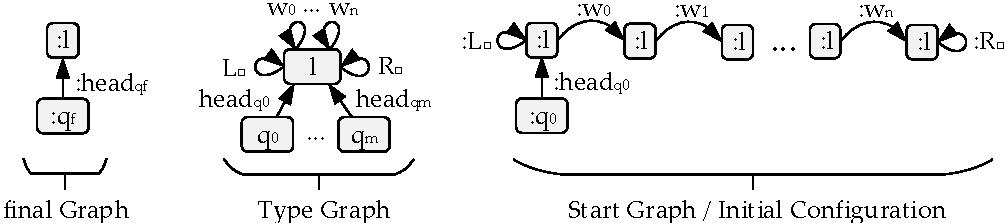
\includegraphics[width=.92\textwidth]{img/software_trans/turing1.pdf}
  \end{center}
  
  For each transition $(q,w) \to (q',w',\alpha) \in \delta$ with $\alpha \in \{L,N,R\}$, a $\delta_{\alpha,q,q',w,w'}$-rule is defined as below.
  Each $\delta$-rule deletes symbol $w$,replaces it by $w'$ and moves the head on the tape one step to the left for $\alpha=L$, to the right for $\alpha=R$ or performs no move for $\alpha=N$ by deleting the old head and state $q$ and replacing them by the new state $q'$ and head pointing to the new tape position.
  
  \begin{center}
  \begin{tikzpicture}
  \node[inner sep=0pt] (a) at (0,0) {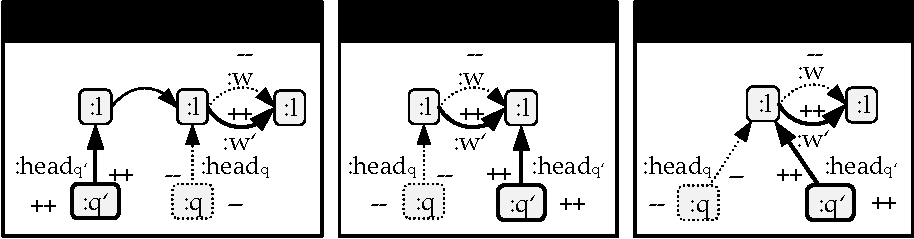
\includegraphics[width=.8\textwidth]{img/software_trans/turing2.pdf}};
  \node[inner sep=0pt] (b) at (-4.95,1.24) {\textcolor{white}{$\delta_{L,q,q',w,w'}$}};
  \node[inner sep=0pt] (c) at (-.6,1.24) {\textcolor{white}{$\delta_{R,q,q',w,w'}$}};
  \node[inner sep=0pt] (d) at (3.2,1.24) {\textcolor{white}{$\delta_{N,q,q',w,w'}$}};
  \end{tikzpicture}
  \end{center}
  
  Furthermore, the following auxiliary rules are defined:
  \begin{enumerate*}
  \item Rules \code{add-Blank-left} and \code{add-Blank-right} that add a new blank symbol $\Box$ to the right and left ends of the tape,
  \item for each symbol $w \in \Gamma$, a rule \code{del}$_w$ that deletes the symbol from the tape if a final state $q_f$ is reached,
  \item rules \code{del-Blank-left} and \code{del-Blank-right} that delete the markers $L_\Box$ and $R_\Box$ for the left and right ends of the tape if a final state $q_f$ is reached, and
  \item rule \code{del-link} which delets \code{l} nodes if a final state $q_f$ is reached.
  \end{enumerate*}
  
  Therefore, a TM with input $w_0w_1\ldots w_n$ is encoded as start graph $S$ together with the set $P$ of production rules from above forming graph grammar $\GG=(S,P)$ and together with the final graph from above (left) where $q_f$ is the final state.
  Moreover, $P$ is finite by $Q$ and $\Gamma$ being finite for $\delta\colon (Q \setminus q_f) \times \Gamma \to Q \times \Gamma \times \{L,N,R\}$ and the final graph is finite.
  
  \begin{center}
  \begin{tikzpicture}
  \node[inner sep=0pt] (a) at (0,0) {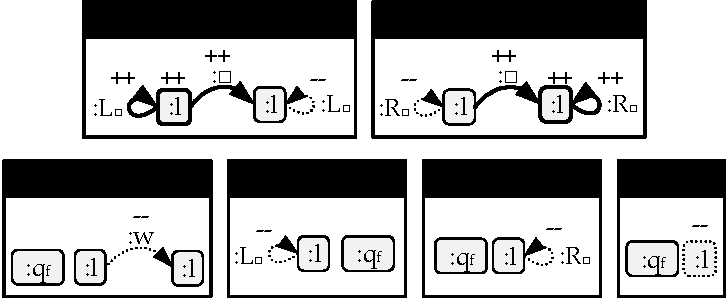
\includegraphics[width=.67\textwidth]{img/software_trans/turing3.pdf}};
  \node[inner sep=0pt] (b) at (-2.6,1.78) {\textcolor{white}{\small{add-Blank-left}}};
  \node[inner sep=0pt] (c) at (1.5,1.78) {\textcolor{white}{\small{add-Blank-right}}};
  \node[inner sep=0pt] (d) at (-4.4,-.42) {\textcolor{white}{\small{del$_w$}}};
  \node[inner sep=0pt] (e) at (-.7,-.42) {\textcolor{white}{\small{del-Blank-left}}};
  \node[inner sep=0pt] (f) at (2.1,-.42) {\textcolor{white}{\small{del-Blank-right}}};
  \node[inner sep=0pt] (g) at (4.2,-.42) {\textcolor{white}{\small{del-link}}};
  \end{tikzpicture}
  \end{center}
  
  Obviously, if the TM reaches the final state $q_f$, then the final graph is (partially) reachable from the start graph.
  This holds, since,
  \begin{enumerate*}
  \item for each transition there exists a dedicated $\delta$-rule simulating the transition,
  \item new blank symbols can be added to the ends of the tape at any time by auxiliary rules \code{del-Blank-left(right)} simulating an infinite tape, and
  \item auxiliary rules \code{del\ldots} finally delete all nodes and edges except the final graph due to the gluing condition.
  \end{enumerate*}
  Conversely, if the final graph is (partially) reachable from the start graph, then the TM reaches the final state $q_f$.
  This holds, since, each graph which is reachable from the start graph follows the structure of the start graph with exactly one state node and head edge, at most one \code{L}$_\Box$ edge and at most one \code{R}$_\Box$ edge at the ends of the tape and at most one symbol edge between each two \code{l} nodes forming a linear tape without branchings via edges.
  Therefore, there is at most one $\delta$-rule applicable to each graph via at most one ($\M$-)match exactly representing the corresponding transition of the TM by the determinism of TM with $\delta$ being a function.
  Thus, each sequence of mixed $\delta$- and \code{add-Blank-left(right)}-rule applications from the start graph to a graph containing (final) state node $q_i$ represents a computation of TM from the initial configuration to a configuration with (final) state $q_i$.
  Finally, when assuming the decidability of the (partial) reachability problem, we could also decide the halting problem leading to a contradiction.
  \item
  \begin{enumerate}
    \item There are at most $\left\vert{M}\right\vert !$ acyclic (terminating) match-paths in $\GS$ (that start in $S$) where each is composed of at most $\left\vert{M}\right\vert$ matches.
      \begin{center}
\begin{tikzpicture}[]
\fill (0,0) node[inner sep=1pt] (Lp) {$L_p$};
\fill (0,0) node[right of=Lp,xshift=1.5cm,inner sep=1pt] (Kp) {$K_p$};
\fill (0,0) node[right of=Kp,xshift=1.5cm,inner sep=1pt] (Rp) {$R_p$};
\fill (0,0) node[below of=Lp,yshift=-1cm,inner sep=1pt] (A1) {$A_1$};
\fill (0,0) node[right of=A1,xshift=1.5cm,yshift=.5cm,inner sep=1pt] (O1) {$O_1$};
\fill (0,0) node[right of=O1,xshift=1.5cm,inner sep=1pt] (B1) {$B_1$};
\fill (0,0) node[below of=A1,yshift=-1cm,inner sep=1pt] (A2) {$A_2$};
\fill (0,0) node[right of=A2,xshift=1.5cm,inner sep=1pt] (O2) {$O_2$};
\fill (0,0) node[right of=O2,xshift=1.5cm,inner sep=1pt] (B2) {$B_2$};
\fill (0,0) node[right of=A1,xshift=1.5cm,yshift=-.5cm,inner sep=1pt] (O) {$O$};
\fill (0,0) node[right of=O,xshift=1.5cm,inner sep=1pt] (B) {$B$};
\fill (0,0) node[below of=B2,inner sep=1pt] (G) {$G$};
%
\fill (0,0) node[right of=A1,xshift=.25cm,yshift=1cm,inner sep=1pt] (1) {$(1)$};
\fill (0,0) node[right of=A1,xshift=.85cm,inner sep=1pt] (2) {$(2)$};
\fill (0,0) node[right of=A1,xshift=.25cm,yshift=-1cm,inner sep=1pt] (3) {$(3)$};
\fill (0,0) node[right of=A1,xshift=3.25cm,yshift=1cm,inner sep=1pt] (4) {$(4)$};
\fill (0,0) node[right of=A1,xshift=3.25cm,inner sep=1pt] (5) {$(5)$};
\fill (0,0) node[right of=A1,xshift=3.25cm,yshift=-1cm,inner sep=1pt] (6) {$(6)$};
%
{
\pgfsetarrows{right hook-latex}
\path (Kp) edge[] node[fill=white]{\scriptsize{$r_p$}} (Rp);
\path (O1) edge[] node[fill=white]{\scriptsize{$r'_{p,1}$}} (B1);
\path (O2) edge[] node[fill=white]{\scriptsize{$r'_{p,2}$}} (B2);
\path (O) edge[dotted] node[fill=white]{\scriptsize{$r'$}} (B);
%
\pgfsetarrows{left hook-latex}
\path (Kp) edge[] node[fill=white]{\scriptsize{$l_p$}} (Lp);
\path (O1) edge[] node[fill=white]{\scriptsize{$l'_{p,1}$}} (A1);
\path (O2) edge[] node[fill=white]{\scriptsize{$l'_{p,2}$}} (A2);
\path (A1) edge[] node[fill=white]{\scriptsize{$i$}} (A2);
\path (O) edge[dotted] node[fill=white]{\scriptsize{$l'$}} (A1);
\path (B2) edge[] node[right]{\scriptsize{$m''$}} (G);
%
\pgfsetarrows{-latex}
\path (Lp) edge[] node[fill=white]{\scriptsize{$n_1 \circ m$}} (A1);
\path (Kp) edge[] node[fill=white]{\scriptsize{$n''_1$}} (O1);
\path (Rp) edge[] node[fill=white]{\scriptsize{$n'_1$}} (B1);
\path (Lp) edge[bend right=55] node[left]{\scriptsize{$n_2 \circ m$}} (A2);
\path (Kp) edge[bend left=55] node[fill=white, xshift=-.25cm,yshift=1.25cm]{\scriptsize{$n''_2$}} (O2);
\path (Rp) edge[bend left=55] node[fill=white]{\scriptsize{$n'_2$}} (B2);
\path (Kp) edge[bend left=35,dotted] node[yshift=.25cm,fill=white]{\scriptsize{$n''$}} (O);
\path (Rp) edge[bend left=35,dotted] node[yshift=.25cm,fill=white]{\scriptsize{$n'$}} (B);
\path (O) edge[dotted] node[fill=white]{\scriptsize{$\underline{n}''$}} (O2);
\path (B) edge[dotted] node[fill=white]{\scriptsize{$\underline{n}'$}} (B2);
\path (O1) edge[dotted] node[left]{\scriptsize{$o$}} (O);
\path (B1) edge[dotted] node[left]{\scriptsize{$b$}} (B);
%
}
\end{tikzpicture}
\end{center}
  Furthermore, given a match-path $\paths$, a graph $G$ and two recursive transformations $A \Trans{\paths}_\GS B$ and $A \Trans{\paths}_\GS B'$, then $\exists m'\colon B \to G \in \M$ if and only if $\exists m''\colon B' \to G \in \M$ $^{(*^1)}$, i.e., $\nexists m'$ implies $\nexists m''$ for all other recursive transformations w.r.t. $\paths$.\thispagestyle{plain}
  Therefore, for verifying all acyclic, terminating recursive transformations that start in $S$ whether $m$ exists, it is sufficient to verify only one recursive transformation for each match-path.
  By a finite set of acyclic, terminating match-paths in $\GS$ that start in $S$, each path being finite and $G$ being finite, the verification terminates.
  For showing $(*^1)$, we show it analogously for a single recursive transformation step which directly implies $(*^1)$ by induction over the recursive transformations.
  Thus, given a match $m$, a production $p=(L_p \transB{l_p} K_p \trans{r_p} R_p)$, a graph $G$ and two recursive transformation steps $A_1 \Trans{(p,m,n_1)}_{\GS,n'_1} B_1$ and $A_2 \Trans{(p,m,n_2)}_{\GS,n'_2} B_2$ with $i\colon A_1 \to A_2 \in \M$ and $i \circ n_1 \circ m=n_2 \circ m$, if $\exists m''\colon B_2 \to G \in \M$, then $\exists m'=m'' \circ \underline{m}' \in \M$ with $\underline{m}'\colon B_1 \to B_2 \in \M$ and $\underline{m}' \circ n'_1=n'_2$.
  By the restriction theorem with $i \in \M$ and $i \circ n_1 \circ m=n_2 \circ m$, there exists pushouts $(1)+(2),(3),(4)+(5)$ and $(6)$ with $\underline{n}'' \circ n''=n''_2$ and $\underline{n}' \circ n'=n'_2$.
  By $(\cat{\AGraphs_\ATGI},\M)$ being $\M$-adhesive, uniqueness of pushout complements and $(1)$ as well as $(1)+(2)$ being pushouts, there is induced isomorphism $o\colon O_1 \to O$ with $o \circ n''_1=n''$.
  By pushout decomposition with $(1)+(2)+(3)$ and $(1)$ being pushouts, $(2)+(3)$ is a pushout.
  By $\M$ being closed under pushouts, $\underline{n}'' \circ o \in \M$.
  By $(4)$ and $(4)+(5)$ being pushouts, there is induced morphism $b\colon B_1 \to B$ with $b \circ n'_1=n'$ by universal pushout property.
  By pushout decomposition with $(4)+(5)+(6)$ and $(4)$ being pushouts, $(5)+(6)$ is a pushout.
  Thus, $\underline{m}'=\underline{n}' \circ b \in \M$ with $\underline{m}' \circ n'_1=n'_2$, since, $\M$ is closed under pushouts.
  Finally, $m'' \circ \underline{m}' \in \M$ by $\M$-composition.
  \item For cyclic, terminating recursive transformations that start in $S$ we conclude as follows.
  By $(*^1)$, the verification of a single recursive transformation for each match-path again encloses the verification of all recursive transformations.
  The verification procedure of whether $m \in \M$ exists is as follows:
  Given $t\colon A \Trans{\paths}_{\GS,n'} B$ with $n'\colon R \to B \in \M$ - we start at $S$ with the empty path $\paths$ and $n'=\id_S\colon S \to S$.
  Then, there are at most $(\left\vert{M}\right\vert^{\left\vert{M}\right\vert})^k\cdot \left\vert{M}\right\vert$ match-paths for some $k \in \mathbb{N}$ that may extend $\paths$ by up to $\left\vert{M}\right\vert \cdot k + 1$ matches.
  For each possible $\paths$ extension via matches $(m_i)_{i \in \{1\ldots l \leq \left\vert{M}\right\vert \cdot k + 1\}}$, $t$ is extended match-wise via recursive transformation steps $s_i\colon (A_i \Trans{(s_\GS(m_i),m_i,n'_{i-1})}_{\GS,n'_i} B_i)_{i \in \{1\ldots l\}}$ with $n'_0=n'$ and $A_0=B$.
  If there is some $m_i$ in an extension such that the corresponding step $s_i$ does not exist due to a violation of the gluing condition, then we stop for this specific extension.
  If there is some $x \in n'_{i-1}(\_)$ that is preserved along $\der(s_i)$ but $x \not\in n'_i(\_)$ (i.e., $B$ is strongly extended by element $x$), then we recursively proceed with the verification procedure for this specific extension with $t=t'$ where $t'$ is $t$ extended up to $s_i$ and $n'=n'_i$.
  Note that $x$ will never be touched (deleted) in any further extensions.
  Thus, by this monotonicity in recursive transformations we can stop for a specific extension if we reach a graph in that extension that is composed out of $x$'s and is larger than $G$.
  If we have applied the last possible step $s_{\left\vert{M}\right\vert \cdot k + 1}$ in an extension, then it is true that there is a match $m_i\colon L \to C \in M$ which was visited at least $k + 1$ times in that extension via some step $s_i$ with $k=\left\vert{C}\right\vert!$ and $\left\vert{C}\right\vert$ being the sum of graph elements (nodes and edges) in $C$.
  Furthermore, the graph which is obtained by $s_i$ is isomorphic to each graph which was obtained by any of the previous steps via $m_i$, since, the graphs where not strongly extended by some element and we have already obtained all possible $k=\left\vert{C}\right\vert !$ combinations of mapping the elements of $C$ to $C$.
  Thus, it is guaranteed that we repeat one of these combinations with $k+1$ and therefore, can stop for this specific extension.
  Therefore, the overall procedure terminates.
  \qed
  \end{enumerate}
\end{enumerate}

\section{Proof of \cref{sec-dc-general-rec,prop:sec-compl-software-trans:weakened_lang_well_def}}
\label{sec-proofs:prop:sec-compl-software-trans:weakened_lang_well_def}
The base-path $b_{\paths'}$ of a match-path $\paths'=(m_1\ldots m_n)$ and the partial mapping $\rightharpoonup_{\paths'}\colon \{1\ldots n\} \to \{1\ldots n\}$ of positions of matches from $\paths'$ to $b_{\paths'}$ are given by $b_{\paths'}:=b(\varnothing,0,1,\paths')$ with
\begin{center}
\text{for }$j \leq n, b(m,i,j,\paths'=(m_1\ldots m_i,m_{i+1} \ldots m_j \ldots m_k \ldots m_n)):=$\\
$\begin{cases}
b(m,i,j+1,\paths') & \text{if $i > 0$ and $(m_{i+1}\ldots m_j \ldots m_k)$ is a match-cycle,}\\
b((m,m_j),j,j+1,\paths') & \text{otherwise with } \rightharpoonup_{\paths'}(j):=\left\vert{m}\right\vert + 1
\end{cases}$
\\and for $j > n, b(m,i,j,\paths'=(m_1\ldots m_n)):=m$  
\end{center}
Obviously, if $\paths'$ is acyclic, then $b_{\paths'}=\paths'$ $^{(*^1)}$.\thispagestyle{plain}
Moreover, if $\paths'$ is cyclic, terminating, starts in $A$ or ends in $B$, then $b_{\paths'}$ is acyclic, terminating, starts in $A$ or ends in $B$ $^{(*^2)}$.
We show for general terminating match-paths $\paths'=(m_1\ldots m_n)$, sequences of recursive transformation steps $t'\colon (A_{i-1} \Trans{(s_\GS(m_i),m_i,n_{i-1})}_{\GS,n_i} A_i)_{i \in \{j\ldots n\}}$ over $(m_j\ldots m_n)$ and morphisms $\ac'\colon A \to A_{j-1}$ for $1 \leq j \leq n$ with $(j,\_) \in \rightharpoonup_{\paths'}$ that there is $(\ac\colon A \to B,n) \in \underline{\Lang}_w(b_{\paths'},\rightharpoonup_{\paths'}(j),\ac',n_{j-1},\_)$ such that there is $i\colon B \to A_n \in \M$ with $i \circ \ac=\der(t') \circ \ac'$ and $i \circ n = n_n$ $^{(*^3)}$.
Moreover, if $(m_j\ldots. m_n)$ is acyclic, then $\ac=\der(t') \circ \ac'$ and $n=n_n$ which does also hold for non-terminating $(m_1\ldots m_j\ldots. m_n)$ $^{(*^4)}$.
\begin{enumerate}
  \item[\textbf{Case}] \textbf{($(m_j\ldots m_n)$ is acyclic)}
  By assumption $(j,\_) \in \rightharpoonup_{\paths'}$, $b_{\paths'}=(m_1\ldots m_{j'}\ldots m_{n'})$ with $n-j=n'-j'$, $(m_{j+i}=m_{j'+i})_{i \in \{0\ldots n-j\}}$ and $(\rightharpoonup_{\paths'}(j+i)=j'+i)_{i \in \{0\ldots n-j\}}$ $^{(*^5)}$, since by the construction of $b_{\paths'}$, assuming the opposite for some $j+i$ with $i > 0 $ implies a match-cycle contradicting with assumption $(m_j\ldots m_n)$ being acyclic.
  By induction over $t'$:
  \textbf{Basis.} Let $j=n$, i.e., $t'$ be given by a single recursive transformation step $t'\colon A_{n-1} \Trans{(s_\GS(m_n),m_n,n_{n-1})}_{\GS,n_n} A_n$.
  \textbf{Case ($\mathcal{P}=\varnothing$ or $k=2$)} By construction of $\underline{\Lang}_w$ and $(*^5)$ with $\rightharpoonup_{\paths'}(n)=n'$, $b_{\paths'}=(m_1\ldots m_{n'})$ and $m_n=m_{n'}$, $(\der(t')\circ \ac',n_n) \in \underline{\Lang}_w(b_{\paths'},\rightharpoonup_{\paths'}(j),\ac',n_{j-1},\_)$.
  Finally, $i=\id_{A_n} \in \M$ with $\id_{A_n} \circ \der(t') \circ \ac'=\der(t') \circ \ac'$ and $\id_{A_n} \circ n_n=n_n$.
  \textbf{Case ($\mathcal{P}\neq\varnothing$)} By $(\ac',n_{j-1}) \in \mathcal{C}$, it leads to the previous case with switch $k=2$.
  \textbf{Hypothesis.} Assume that $(*^4)$ holds for $t'$ consisting of $1 \leq k < n$ steps with $j=(n+1)-k$.
  \textbf{Step.} Let $j=(n+1)-(k+1)=n-k$, i.e., $t'$ consists of $k+1$ steps.
  Analogously to the basis by $(*^5)$ with $m_{n-k}=m_j=m_{j'}=m_{\rightharpoonup_{\paths'}(j)} \in b_{\paths'}$, there is some invocation $\underline{\Lang}_w(b_{\paths'},\rightharpoonup_{\paths'}(n-k)+1,\der(\overline{t}) \circ \ac',n_{n-k},\_) \stackrel{(*^5)}{=} \underline{\Lang}_w(b_{\paths'},\rightharpoonup_{\paths'}((n+1)-k),\der(\overline{t}) \circ \ac',n_{n-k},\_)$ from $\underline{\Lang}_w(b_{\paths'},\rightharpoonup_{\paths'}(j),\ac',n_{j-1},\_)$ with $\overline{t}\colon A_{n-k-1} \Trans{(s_\GS(m_{n-k}),m_{n-k},n_{n-k-1})}_{\GS,n_{n-k}} A_{n-k}$, $\overline{t}'\colon (A_{i-1} \Trans{(s_\GS(m_i),m_i,n_{i-1})}_{\GS,n_i} A_i)_{i \in \{(n+1)-k\ldots n\}}$ and $\der(\overline{t}') \circ \der(\overline{t})=\der(t')$.
  By hypothesis and \cref{prop:sec-compl-software-trans:decomp_acyclic_match-paths} together with acyclic $(m_j\ldots m_n)$ implying $(m_{j+1}\ldots m_n)=(m_{(n+1)-k}\ldots m_n)$ being acyclic, $(\der(\overline{t}') \circ \der(\overline{t}) \circ \ac',n_n)=(\der(t') \circ \ac',n_n) \in \underline{\Lang}_w(b_{\paths'},\rightharpoonup_{\paths'}((n+1)-k),\der(\overline{t})\circ \ac',n_{n-k},\_)$ and therefore, $(\der(t') \circ \ac',n_n) \in \underline{\Lang}_w(b_{\paths'},\rightharpoonup_{\paths'}(j),\ac',n_{j-1},\_)$.
  Finally, $i=\id_{A_n} \in \M$ with $\id_{A_n} \circ \der(t') \circ \ac'=\der(t') \circ \ac'$ and $\id_{A_n} \circ n_n=n_n$.
  \item[\textbf{Case}] \textbf{($(m_j\ldots m_n)$ is cyclic)}\newline
  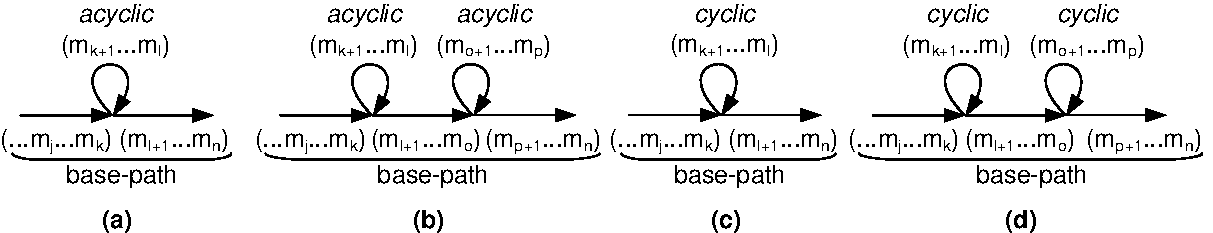
\includegraphics[width=.95\textwidth]{img/software_trans/proof3.pdf}
  By induction over the structure of $t'$ based on Basis (a) and Steps (b)-(d) from above:
  Sub-paths $(m_{l+1}\ldots m_n)$ or $(m_{p+1}\ldots m_n)$ with $l,p < n$ in (a)-(d) are guaranteed to be in the base-path of $\paths'$, respectively, since, assuming they were part of a match-cycle contradicts with the assumption that $\paths'$ is terminating.
  Furthermore by assumption $(j,\_) \in \rightharpoonup_{\paths'}$, sub-paths $(m_j\ldots m_k)$ with $j \leq k$ in (a)-(d) are guaranteed to be in the base-path of $\paths'$, respectively.
  Let $(m_j\ldots m_n)$ be composed of sub-paths $(m_j\ldots m_k),(m_{k+1}\ldots m_l),(m_{l+1}\ldots m_n)$ or $(m_j\ldots m_k),(m_{k+1}\ldots m_l),(m_{l+1}\ldots m_o),(m_{o+1}\ldots m_p),(m_{p+1}\ldots m_n)$, respectively, with $(m_{k+1}\ldots m_l) \in \Paths_{t_\GS(m_{l+1}),t_\GS(m_{l+1})}(\GS)$ and $(m_{o+1}\ldots m_p) \in \Paths_{t_\GS(m_{p+1}),t_\GS(m_{p+1})}(\GS)$ being (a)cyclic match-cycles and $b_{\paths'}=(\ldots m_j\ldots m_k,m_{l+1}\ldots m_n)$ or $b_{\paths'}=(\ldots m_j\ldots m_k,m_{l+1}\ldots m_o,m_{p+1}\ldots m_n)$ being the base-paths of $\paths'$.
  Thus, the sequence $t'$ of steps is given by sub-sequences $t'_{(y,z)}\colon (A_{i-1} \Trans{(s_\GS(m_i),m_i,n_{i-1})}_{\GS,n_i} A_i)_{i \in \{y\ldots z\}}$ for $(y,z) \in \{(j,k),(k+1,l),(l+1,n)\}$ or $(y,z) \in \{(j,k),(k+1,l),(l+1,o),(o+1,p),(p+1,n)\}$, respectively.
  \textbf{Basis.} 
  %By $P$ being non-deleting, the gluing condition is satisfied by each match $n_{i-1} \circ m_i$ and therefore, $t'_{(j,k)}$ can be extended to a sequence $t''\colon (A'_{i-1} \Trans{(s_\GS(m_i),m_i,n'_{i-1})}_{\GS,n'_i} A'_i)_{i \in \{j\ldots k\ldots n-l\}}$ over $b_{\paths'}$ with $A'_{i-1}=A_{i-1},A'_i=A_i,n'_{i-1}=n_{i-1}$ and $n'_i=n_i$ for $i \in \{j\ldots k\}$, since, pushouts exist along $\M$-morphisms $s_\GS(m_i)$.
  By \cref{prop:sec-compl-software-trans:decomp_acyclic_match-paths} and $b_{\paths'}$ being acyclic by $(*^2)$, $(m_j\ldots m_k,m_{l+1}\ldots m_n)$ and therefore, $(m_j\ldots m_k)$ are acyclic and furthermore, $b_{\paths'}\stackrel{(*^1)}{=} b_{b_{\paths'}}$.
  %Moreover, $b_{\paths'}$ is terminating by $(*^2)$ with $\paths'$ being terminating by assumption and $b_{\paths'}\stackrel{(*^1)}{=} b_{b_{\paths'}}$.
  Thus, by $(*^4)$ %and \cref{rem:sec-gc-gc:der_span_non_deleting}
  , $(\der(t'_{(j,k)}) \circ \ac',n_{k}) \in \underline{\Lang}_w((\ldots m_j\ldots m_k),\rightharpoonup_{\paths'}(j),\ac',n_{j-1},\_)$.
  Therefore, by the match-wise construction of $\underline{\Lang}_w$, there is an invocation $\underline{\Lang}_w(b_{\paths'},\rightharpoonup_{\paths'}(l+1),\der(t'_{(j,k)}) \circ \ac',n_k,\_)$ from $\underline{\Lang}_w(b_{\paths'},\rightharpoonup_{\paths'}(j),\ac',n_{j-1},\_)$.
  Assume that match-cycle $m=(m_{k+1}\ldots m_l) \in \gg_\GS(b_{\paths'})$, then $m_n \in m$ by the definition of $\gg_\GS$ and therefore, $b_{\paths'}$ is not terminating contradicting with the direct implication of assumption $\paths'$ being terminating via $(*^2)$.
  Thus, from $m \not\in \gg_\GS(b_{\paths'})$ and $m$ being acyclic by assumption, we conclude that $m \in \mathcal{P} \subseteq \Paths_{t_\GS(m_{\rightharpoonup_{\paths'}(l+1)}),t_\GS(m_{\rightharpoonup_{\paths'}(l+1)})}(\GS) \setminus \gg_\GS(b_{\paths'})$.
  We inductively conclude over sequence $t'_{(k+1,l)}$ as follows:
    \begin{center}
\begin{tikzpicture}[]
\fill (0,0) node[inner sep=1pt] (Ljp1) {$L_{k+1}$};
\fill (0,0) node[right of=Ljp1,xshift=1.5cm,inner sep=1pt] (Rjp1) {$R_{k+1}$};
\fill (0,0) node[below of=Ljp1,inner sep=1pt] (Rj) {$R_k$};
\fill (0,0) node[below of=Rj,inner sep=1pt] (Aj) {$A_k$};
\fill (0,0) node[right of=Aj,xshift=1.5cm,inner sep=1pt] (Ajp1) {$A_{k+1}$};
\fill (0,0) node[above of=Rjp1,inner sep=1pt] (Ljp2) {$L_{k+2}$};
\fill (0,0) node[right of=Ljp2,xshift=1.5cm,inner sep=1pt] (Rjp2) {$R_{k+2}$};
\fill (0,0) node[right of=Ajp1,xshift=1.5cm,inner sep=1pt] (Ajp2) {$A_{k+2}$};
\fill (0,0) node[right of=Rj,xshift=1cm,inner sep=1pt] (R'jp1) {$R'_{k+1}$};
\fill (0,0) node[right of=R'jp1,xshift=1cm,inner sep=1pt] (R'jp2) {$R'_{k+2}$};
\fill (0,0) node[right of=Rjp1,xshift=1cm,inner sep=1pt] (L'jp2) {$L'_{k+2}$};
%
\fill (0,0) node[right of=Ljp1,xshift=0cm,yshift=-.5cm,inner sep=1pt] (1) {$(1)$};
\fill (0,0) node[right of=Rj,xshift=0cm,yshift=-.5cm,inner sep=1pt] (2) {$(2)$};
\fill (0,0) node[right of=Ljp2,xshift=-.25cm,yshift=-.5cm,inner sep=1pt] (3) {$(3)$};
\fill (0,0) node[right of=Rjp1,xshift=-.25cm,yshift=-.5cm,inner sep=1pt] (4) {$(4)$};
\fill (0,0) node[right of=Ajp1,xshift=-.25cm,yshift=.5cm,inner sep=1pt] (5) {$(5)$};
%
\fill (0,0) node[right of=Rjp2,xshift=2cm,yshift=1cm,inner sep=1pt] (Li) {$L_i$};
\fill (0,0) node[right of=Li,xshift=2cm,inner sep=1pt] (Ri) {$R_i$};
\fill (0,0) node[below of=Li,inner sep=1pt] (Rim1) {$R_{i-1}$};
\fill (0,0) node[below of=Rim1,inner sep=1pt] (A1) {};
\fill (0,0) node[below of=A1,inner sep=1pt] (A2) {};
\fill (0,0) node[below of=A2,inner sep=1pt] (Aim1) {$A_{i-1}$};
\fill (0,0) node[right of=Aim1,xshift=2cm,inner sep=1pt] (Ai) {$A_i$};
\fill (0,0) node[below of=Rim1,xshift=-.5cm,inner sep=1pt] (L'im1) {$L'_{i-1}$};
\fill (0,0) node[below of=L'im1,xshift=-.5cm,inner sep=1pt] (R'im1) {$R'_{i-1}$};
\fill (0,0) node[right of=L'im1,xshift=1.5cm,inner sep=1pt] (L'i) {$L'_i$};
\fill (0,0) node[right of=R'im1,xshift=1.5cm,inner sep=1pt] (R'i) {$R'_i$};
%
\fill (0,0) node[right of=Rim1,xshift=0cm,yshift=0cm,inner sep=1pt] (6) {$(6_i)$};
\fill (0,0) node[right of=R'im1,xshift=1cm,yshift=.5cm,inner sep=1pt] (7) {$(7_i)$};
\fill (0,0) node[right of=Aim1,xshift=0cm,yshift=.5cm,inner sep=1pt] (8) {$(8_i)$};
%
{
\pgfsetarrows{right hook-latex}
\path (Ljp1) edge[] node[]{\scriptsize{}} (Rjp1);
\path (Aj) edge[] node[]{\scriptsize{}} (Ajp1);
\path (Ajp1) edge[] node[]{\scriptsize{}} (Ajp2);
\path (Ljp2) edge[] node[]{\scriptsize{}} (Rjp2);
\path (Ljp1) edge[] node[left]{\scriptsize{$m_{k+1}$}} (Rj);
\path (Ljp2) edge[] node[left]{\scriptsize{$m_{k+2}$}} (Rjp1);
\path (Rj) edge[] node[left]{\scriptsize{$n_k$}} (Aj);
\path (Rjp1) edge[] node[right, yshift=-.25cm]{\scriptsize{$n_{k+1}$}} (Ajp1);
\path (Rjp2) edge[] node[right]{\scriptsize{$n_{k+2}$}} (Ajp2);
\path (Rjp1) edge[dotted] node[left]{\scriptsize{$r_{k+1}$}} (R'jp1);
\path (Rj) edge[dotted] node[above,yshift=-.1cm]{\scriptsize{$g_{k+1}$}} (R'jp1);
\path (R'jp1) edge[dotted] node[above,yshift=-.1cm]{\scriptsize{$g_{k+2}$}} (R'jp2);
\path (Rjp2) edge[dotted] node[left]{\scriptsize{$l_{k+2}$}} (L'jp2);
\path (Rjp1) edge[dotted] node[]{\scriptsize{}} (L'jp2);
\path (L'jp2) edge[dotted] node[left]{\scriptsize{$r_{k+2}$}} (R'jp2);
\path (R'jp1) edge[dotted] node[left]{\scriptsize{$a_{k+1}$}} (Ajp1);
\path (R'jp2) edge[dotted] node[left]{\scriptsize{$a_{k+2}$}} (Ajp2);
%
\path (Li) edge[] node[left]{\scriptsize{$m_i$}} (Rim1);
\path (Rim1) edge[] node[fill=white]{\scriptsize{$n_{i-1}$}} (Aim1);
\path (Rim1) edge[] node[left]{\scriptsize{$l_{i-1}$}} (L'im1);
\path (L'im1) edge[] node[left]{\scriptsize{$r_{i-1}$}} (R'im1);
\path (R'im1) edge[] node[left]{\scriptsize{$a_{i-1}$}} (Aim1);
\path (Li) edge[] node[left]{\scriptsize{}} (Ri);
\path (L'im1) edge[dotted] node[left]{\scriptsize{}} (L'i);
\path (Ri) edge[dotted] node[left]{\scriptsize{$l_i$}} (L'i);
\path (R'im1) edge[dotted] node[fill=white]{\scriptsize{$g_i$}} (R'i);
\path (L'i) edge[dotted] node[left]{\scriptsize{$r_i$}} (R'i);
\path (Ri) edge[] node[fill=white]{\scriptsize{$n_i$}} (Ai);
\path (R'i) edge[dotted] node[left]{\scriptsize{$a_i$}} (Ai);
\path (Aim1) edge[] node[]{\scriptsize{}} (Ai);
%
\pgfsetarrows{left hook-latex}
%
\pgfsetarrows{-latex}
%
}
\end{tikzpicture}
\end{center} 
  All given morphisms from above are in $\M$ by the definition of non-deleting productions and recursive transformation steps.
  Therefore, we can construct pushouts over them resulting again in $\M$-morphisms only, since, $\M$ is closed under pushouts.
  In particular, we construct pushout $(1)$ with induced morphism $a_{k+1}$ and $a_{k+1} \circ r_{k+1}=n_{k+1}$.
  By pushout decomposition with $(1)+(2)$ and $(1)$ being pushouts, $(2)$ is a pushout.
  We construct pushouts $(3)$ and $(4)$ resulting in pushout $(3)+(4)$ by pushout composition with induced morphism $a_{k+2}$ and $a_{k+2} \circ r_{k+2} \circ l_{k+2}=n_{k+2}$.
  Again, by pushout decomposition with $(3)+(4)+(5)$ and $(3)+(4)$ being pushouts, $(5)$ is a pushout.
  Analogously, for each subsequent step $i$ with $k+2 < i \leq l$ in $t'_{(k+1,l)}$, we construct pushouts $(6_i)$ over $l_{i-1}\circ m_i \in \M$ by $\M$-composition and $(7_i)$ resulting again in pushouts $(6_i)+(7_i)$ and $(8_i)$ with induced morphism $a_i$ and $a_i \circ r_i \circ l_i=n_i$.
  Thus, by $(*^4)$ for $m\stackrel{(*^1)}{=}b_m$, $(g_l \circ \ldots \circ g_{k+1},r_l \circ l_l) \in B_m=\underline{\Lang}_w(m,1,\id_{R_k},\id_{R_k},2)$ in \cref{def:sec-compl-software-trans:weakened_lang,item:sec-compl-software-trans:weakened_lang:2a}.
  Furthermore, for $t'_{(k+1,l)}$ by pushout composition, we obtain pushouts $(1)+(4)+(7_{k+3})+\ldots +(7_l)$ and $(2)+(5)+(8_{k+3})+\ldots +(8_l)$ and the composition of both.
  Therefore, the pushout complement exists in \cref{def:sec-compl-software-trans:weakened_lang,item:sec-compl-software-trans:weakened_lang:2c} with induced morphism $l_l \in \M$.
  Since, the pushout complement and object in \cref{def:sec-compl-software-trans:weakened_lang,item:sec-compl-software-trans:weakened_lang:2b} are unique up to isomorphism, w.l.o.g. we conclude that $(\der(t'_{(k+1,l)}) \circ \der(t'_{(j,k)}) \circ \ac',n_l) \in A_k \oplus B_m \subseteq \mathcal{C}$ for the trivial $i_{L_{k+1}}$-$\M$-decomposition $d=(I_{L_{k+1}} \trans{i_{L_{k+1}}} L_{k+1} \trans{\id_{L_{k+1}}} L_{k+1}) \in \mathcal{D}$ in \cref{def:sec-compl-software-trans:weakened_lang,item:sec-compl-software-trans:weakened_lang:1} with $m=m_{k+1}$ in \cref{def:sec-compl-software-trans:weakened_lang}.
  Note that for $\der(t)=n'=\id_{R_k}$ in \cref{def:sec-compl-software-trans:weakened_lang,item:sec-compl-software-trans:weakened_lang:2e}, \cref{def:sec-compl-software-trans:weakened_lang,item:sec-compl-software-trans:weakened_lang:2e1} holds, since, $o'$ is an isomorphism by preservation of isomorphism $\id_{L_{k+1}}$ along the constructed pushout $(o,o')$ with inverse isomorphism $a''=o'^{-1}$ - \cref{def:sec-compl-software-trans:weakened_lang,item:sec-compl-software-trans:weakened_lang:2e2,item:sec-compl-software-trans:weakened_lang:2e3} follow directly from $a''$ being an isomorphism.
  Therefore, there is an invocation $\underline{\Lang}_w(b_{\paths'},\rightharpoonup_{\paths'}(l+1),\der(t'_{(k+1,l)}) \circ \der(t'_{(j,k)}) \circ \ac',n_l,2)$ from $\underline{\Lang}_w(b_{\paths'},\rightharpoonup_{\paths'}(j),\ac',n_{j-1},\_)$.
  By \cref{prop:sec-compl-software-trans:decomp_acyclic_match-paths} and $b_{\paths'}$ being acyclic by $(*^2)$, $(m_{l+1}\ldots m_n)$ is acyclic.
  Therefore by $(*^4)$ with $b_{b_{\paths'}} \stackrel{(*^1)}{=} b_{\paths'}$, $(\der(t'_{(l+1,n)}) \circ \der(t'_{(k+1,l)}) \circ \der(t'_{(j,k)}) \circ \ac',n_n)=(\der(t') \circ \ac',n_n) \in \underline{\Lang}_w(b_{\paths'},\rightharpoonup_{\paths'}(l+1),\der(t'_{(k+1,l)}) \circ \der(t'_{(j,k)}) \circ \ac',n_l,2)$.
  Thus, $(\der(t') \circ \ac',n_n) \in \underline{\Lang}_w(b_{\paths'},\rightharpoonup_{\paths'}(j),\ac',n_{j-1},\_)$.
  \textbf{Hypothesis.}
  Assume that $(*^4)$ and therefore $(*^3)$ with $i$ being the corresponding identity morphism hold for case (a).
  \textbf{Step.}
  Analogously to the base case, for case (b), there is an invocation $\underline{\Lang}_w(b_{\paths'},\rightharpoonup_{\paths'}(l+1),\der(t'_{(k+1,l)}) \circ \der(t'_{(j,k)}) \circ \ac',n_l,2)$ from $\underline{\Lang}_w(b_{\paths'},\rightharpoonup_{\paths'}(j),\ac',n_{j-1},\_)$.
  By induction hypothesis, $(\der(t') \circ \ac',n_n) \in \underline{\Lang}_w(b_{\paths'},\rightharpoonup_{\paths'}(l+1),\der(t'_{(k+1,l)}) \circ \der(t'_{(j,k)}) \circ \ac',n_l,2)$ and therefore, $(\der(t') \circ \ac',n_n) \in \underline{\Lang}_w(b_{\paths'},\rightharpoonup_{\paths'}(j),\ac',n_{j-1},\_)$.
  Analogously, we inductively proceed with arbitrary acyclic match-cycles that are reachable from $b_{paths'}$.
  For case (c) with cyclic match-path $(m_{k+1}\ldots m_l)$, let $(m_{l'}\ldots m_l)$ in $(m_{k+1}\ldots m_{l'}\ldots m_l)$ with $t_\GS(m_{l'})=t_\GS(m_{k+1})$ and $\forall i \in \{l'+1\ldots l\}.t_\GS(m_i) \neq t_\GS(m_{l'})$ $^{(*^6)}$ be the last match-cycle in $(m_{k+1}\ldots m_l)$ that starts and ends in $t_\GS(m_{l+1})$.
  Analogously to the base case, there is an invocation $\underline{\Lang}_w(b_{\paths'},\rightharpoonup_{\paths'}(l+1),\der(t'_{(j,k)}) \circ \ac',n_k,\_)$ from $\underline{\Lang}_w(b_{\paths'},\rightharpoonup_{\paths'}(j),\ac',n_{j-1},\_)$.
  Based on the construction in \cref{def:sec-compl-software-trans:weakened_lang} we conclude as follows:
      \begin{center}
\begin{tikzpicture}[]
\fill (0,0) node[inner sep=1pt] (Lkp1) {$L_{k+1}$};
\fill (0,0) node[right of=Lkp1,xshift=.5cm,inner sep=1pt] (Rkp1) {$R_{k+1}$};
\fill (0,0) node[right of=Rkp1,xshift=-.25cm,inner sep=1pt] (etc1) {$\ldots$};
\fill (0,0) node[right of=etc1,xshift=-.25cm,inner sep=1pt] (Rl'm2) {$R_{l'-2}$};
\fill (0,0) node[below of=Lkp1,inner sep=1pt] (Rk) {$R_k$};
\fill (0,0) node[right of=Rk,xshift=.5cm,inner sep=1pt] (dot2) {$\circ$};
\fill (0,0) node[right of=dot2,xshift=-.25cm,inner sep=1pt] (etc2) {};
\fill (0,0) node[right of=etc2,xshift=-.25cm,inner sep=1pt] (dot3) {$\circ$};
\fill (0,0) node[right of=dot3,xshift=.5cm,inner sep=1pt] (R'') {$R'_{l'-1}=R''$};
\fill (0,0) node[above of=Rl'm2,inner sep=1pt] (Ll'm1) {$L_{l'-1}$};
\fill (0,0) node[right of=Ll'm1,xshift=.5cm,inner sep=1pt] (Rl'm1) {$R_{l'-1}=R_k$};
\fill (0,0) node[left of=Rk,xshift=.25cm,inner sep=1pt] (dert) {$\der(t)\colon$};
\fill (0,0) node[below of=Rk,inner sep=1pt] (Ak) {$A_k$};
\fill (0,0) node[right of=Ak,xshift=.5cm,inner sep=1pt] (Akp1) {$A_{k+1}$};
\fill (0,0) node[right of=Akp1,xshift=-.25cm,inner sep=1pt] (AA) {$\ldots$};
\fill (0,0) node[right of=AA,xshift=-.25cm,inner sep=1pt] (Al'm2) {$A_{l'-2}$};
\fill (0,0) node[right of=Al'm2,xshift=.5cm,inner sep=1pt] (Al'm1b) {$A_{l'-1}$};
%
\fill (0,0) node[right of=Ak,xshift=-.25cm,yshift=.5cm,inner sep=1pt] (1) {$(k+1)$};
\fill (0,0) node[right of=Al'm2,xshift=-.25cm,yshift=.5cm,inner sep=1pt] (2) {$(l'-1)$};
%
\fill (0,0) node[right of=Rl'm2,xshift=2.75cm,inner sep=1pt] (Ll') {$L_{l'}$};
\fill (0,0) node[right of=Ll',xshift=.5cm,inner sep=1pt] (Rl') {$R_{l'}$};
\fill (0,0) node[right of=Rl',xshift=-.25cm,inner sep=1pt] (etc1b) {$\ldots$};
\fill (0,0) node[right of=etc1b,xshift=-.25cm,inner sep=1pt] (c1) {$\circ$};
\fill (0,0) node[below of=Ll',inner sep=1pt] (Rl'm1b) {$R_{l'-1}$};
\fill (0,0) node[below of=Rl'm1b,inner sep=1pt] (Al'm1) {$A_{l'-1}$};
\fill (0,0) node[right of=Al'm1,xshift=.5cm,inner sep=1pt] (Al') {$A_{l'}$};
\fill (0,0) node[right of=Al',xshift=-.25cm,inner sep=1pt] (etc2b) {$\ldots$};
\fill (0,0) node[right of=etc2b,xshift=-.25cm,inner sep=1pt] (Alm1) {$A_{l-1}$};
\fill (0,0) node[right of=Alm1,xshift=.5cm,inner sep=1pt] (Al) {$A_l$};
\fill (0,0) node[above of=c1,inner sep=1pt] (Ll) {$L_{l}$};
\fill (0,0) node[right of=Ll,xshift=.5cm,inner sep=1pt] (Rl) {$R_{l}=R_k$};
\fill (0,0) node[right of=c1,xshift=.5cm,inner sep=1pt] (c2) {$\circ$};
\fill (0,0) node[below of=c1,inner sep=1pt] (c3) {$\circ$};
\fill (0,0) node[below of=Rl',inner sep=1pt] (c4) {$\circ$};
\fill (0,0) node[below of=c2,inner sep=1pt] (c5) {$\circ$};
%
\fill (0,0) node[right of=Al'm1,xshift=-.25cm,yshift=.5cm,inner sep=1pt] (3) {$(l'_2)$};
\fill (0,0) node[right of=Alm1,xshift=-.25cm,yshift=.5cm,inner sep=1pt] (4) {$(l_2)$};
\fill (0,0) node[right of=Rl'm1b,xshift=-.25cm,yshift=.5cm,inner sep=1pt] (5) {$(l'_1)$};
\fill (0,0) node[right of=c3,xshift=-.25cm,yshift=.5cm,inner sep=1pt] (6) {$(l_1)$};
%
\draw [decorate,decoration={brace,amplitude=10pt},xshift=0pt,yshift=0pt] (5,-2.3) -- (0,-2.3) node [black,midway,yshift=-0.6cm] {\footnotesize $\der(t'_{(k+1,l'-1)})$};
\draw [decorate,decoration={brace,amplitude=10pt},xshift=0pt,yshift=0pt] (11.5,-2.3) -- (6.5,-2.3) node [black,midway,yshift=-0.6cm] {\footnotesize $\der(t'_{(l',l)})$};
%
{
\pgfsetarrows{right hook-latex}
\path (Lkp1) edge[] node[]{\scriptsize{}} (Rkp1);
\path (Lkp1) edge[] node[left]{\scriptsize{$m_{k+1}$}} (Rk);
\path (Rk) edge[] node[above]{\scriptsize{$g_{k+1}$}} (dot2);
\path (dot3) edge[] node[above]{\scriptsize{$g_{l'-1}$}} (R'');
\path (Rl'm2) edge[] node[right]{\scriptsize{}} (dot3);
\path (Ll'm1) edge[] node[left]{\scriptsize{$m_{l'-1}$}} (Rl'm2);
\path (Ll'm1) edge[] node[]{\scriptsize{}} (Rl'm1);
\path (Rl'm1) edge[] node[fill=white,yshift=.25cm]{\scriptsize{$n'=r_{l'-1}\circ l_{l'-1}$}} (R'');
\path (Rkp1) edge[] node[right]{\scriptsize{}} (dot2);
\path (Rk) edge[] node[left]{\scriptsize{$n_k$}} (Ak);
\path (dot2) edge[] node[left]{\scriptsize{}} (Akp1);
\path (Ak) edge[] node[left]{\scriptsize{}} (Akp1);
\path (dot3) edge[] node[left]{\scriptsize{}} (Al'm2);
\path (Al'm2) edge[] node[left]{\scriptsize{}} (Al'm1b);
\path (R'') edge[] node[right]{\scriptsize{$a_{l'-1}$}} (Al'm1b);
\path (Rl'm1) edge[bend left=65] node[fill=white]{\scriptsize{$n_{l'-1}$}} (Al'm1b);
%
\path (Ll') edge[] node[left]{\scriptsize{$m_{l'}$}} (Rl'm1b);
\path (Rl'm1b) edge[] node[left]{\scriptsize{$n_{l'-1}$}} (Al'm1);
\path (Ll') edge[] node[above]{\scriptsize{$b_{l'}$}} (Rl');
\path (Al'm1) edge[] node[fill=white]{\scriptsize{$a'_{l'}$}} (Al');
\path (Alm1) edge[] node[fill=white]{\scriptsize{$a'_l$}} (Al);
\path (Ll) edge[] node[left]{\scriptsize{$l_{l-1} \circ m_l$}} (c1);
\path (Ll) edge[] node[]{\scriptsize{}} (Rl);
\path (Rl') edge[] node[]{\scriptsize{}} (c4);
\path (c4) edge[] node[]{\scriptsize{}} (Al');
\path (c1) edge[] node[]{\scriptsize{}} (c3);
\path (c3) edge[] node[]{\scriptsize{}} (Alm1);
\path (Rl) edge[] node[right]{\scriptsize{$l_l$}} (c2);
\path (c2) edge[] node[right]{\scriptsize{$r_l$}} (c5);
\path (c5) edge[] node[right]{\scriptsize{$a_l$}} (Al);
\path (Rl) edge[bend left=45] node[right]{\scriptsize{$n_l$}} (Al);
\path (c1) edge[] node[above]{\scriptsize{$b_l$}} (c2);
\path (Rl'm1b) edge[] node[fill=white]{\scriptsize{$g_{l'}$}} (c4);
\path (c3) edge[] node[fill=white]{\scriptsize{$g_{l}$}} (c5);
%
\pgfsetarrows{left hook-latex}
%
\pgfsetarrows{-latex}
%
}
\end{tikzpicture}\thispagestyle{plain}
\begin{tikzpicture}[]
\fill (0,0) node[inner sep=1pt] (Rk) {$R_{k}$};
\fill (0,0) node[right of=Rk,inner sep=1pt] (c1) {};
\fill (0,0) node[right of=c1,xshift=-.5cm,inner sep=1pt] (d1) {};
\fill (0,0) node[right of=d1,xshift=-.5cm,inner sep=1pt] (c2) {};
\fill (0,0) node[right of=c2,inner sep=1pt] (R'') {$R''$};
\fill (0,0) node[below of=Rk,inner sep=1pt] (Ak) {$A_k$};
\fill (0,0) node[below of=R'',inner sep=1pt] (Al'm1) {$A_{l'-1}$};
\fill (0,0) node[above of=R'',inner sep=1pt] (Rl'm1) {$R_k$};
\fill (0,0) node[above of=Rl'm1,inner sep=1pt] (Ll') {$L_{l'}$};
\fill (0,0) node[right of=Ll',inner sep=1pt] (c3) {};
\fill (0,0) node[right of=c3,inner sep=1pt] (c5) {$\circ$};
\fill (0,0) node[above of=Rk,inner sep=1pt] (z) {};
\fill (0,0) node[above of=z,inner sep=1pt] (c6) {$I'_{L_{l'}}$};
\fill (0,0) node[left of=c6,inner sep=1pt] (z) {$I_{L_{l'}}$};
\fill (0,0) node[right of=Al'm1,xshift=1cm,yshift=-1cm,inner sep=1pt] (c7) {$\circ$};
\fill (0,0) node[right of=Al'm1,inner sep=1pt] (Al') {};
\fill (0,0) node[right of=Al',inner sep=1pt] (Al) {$C$};
%
\fill (0,0) node[right of=c6,xshift=.5cm,yshift=-1cm,inner sep=1pt] (PB) {$(PB)$};
\fill (0,0) node[right of=R'',xshift=0cm,yshift=1.05cm,inner sep=1pt] (2) {$(1)+(2)$};
\fill (0,0) node[right of=Ak,xshift=.5cm,yshift=.5cm,inner sep=1pt] (1) {\scriptsize{$(k+1)+\ldots + (l'-1)$}};
\fill (0,0) node[left of=Rk,xshift=.25cm,inner sep=1pt] (dert) {$\der(t)\colon$};
%
\fill (0,0) node[right of=c5,xshift=3.5cm,yshift=-1cm,inner sep=1pt] (1Rl) {$R_l$};
\fill (0,0) node[left of=1Rl,xshift=-2cm,inner sep=1pt] (1Ll') {$L_{l'}$};
\fill (0,0) node[right of=1Ll',xshift=1cm,inner sep=1pt] (1c1) {$\circ$};
\fill (0,0) node[below of=1Ll',yshift=-.5cm,inner sep=1pt] (1Rl'm1) {$R_{l'-1}$};
\fill (0,0) node[right of=1Rl'm1,xshift=1cm,inner sep=1pt] (1c2) {$\circ$};
\fill (0,0) node[below of=1Rl'm1,yshift=-.5cm,inner sep=1pt] (1Al'm1) {$A_{l'-1}$};
\fill (0,0) node[right of=1Al'm1,xshift=1cm,inner sep=1pt] (1c3) {$C$};
\fill (0,0) node[right of=1c3,xshift=.75cm,inner sep=1pt] (1C') {$C'$};
\fill (0,0) node[right of=1c1,xshift=2.5cm,inner sep=1pt] (1c4) {$\circ$};
\fill (0,0) node[below of=1c4,yshift=-.5cm,inner sep=1pt] (1c5) {$\circ$};
\fill (0,0) node[below of=1c5,yshift=-.5cm,inner sep=1pt] (1Al) {$A_l$};
%
\fill (0,0) node[right of=1Rl'm1,yshift=.75cm,inner sep=1pt] (11) {$(1)$};
\fill (0,0) node[right of=1Al'm1,yshift=.75cm,inner sep=1pt] (12) {$(2)$};
\fill (0,0) node[right of=1c3,xshift=1cm,yshift=1cm,inner sep=1pt] (13) {$(3)$};
% \fill (0,0) node[right of=1c2,yshift=.75cm,inner sep=1pt] (13) {\scriptsize{$(l'_1)+\ldots +(l_1)$}};
% \fill (0,0) node[right of=1c3,yshift=.75cm,inner sep=1pt] (14) {\scriptsize{$(l'_2)+\ldots +(l_2)$}};
%
{
\pgfsetarrows{right hook-latex}
\path (z) edge[] node[above]{\scriptsize{$i_{L_{l'},1}$}} (c6);
\path (Rk) edge[] node[left]{\scriptsize{$n_k$}} (Ak);
\path (Rk) edge[] node[above]{\scriptsize{$g_{l'-1} \circ \ldots \circ g_{k+1}$}} (R'');
\path (Ak) edge[] node[fill=white]{\scriptsize{$\der(t'_{(k+1,l'-1)})$}} (Al'm1);
\path (R'') edge[] node[right]{\scriptsize{$a_{l'-1}$}} (Al'm1);
\path (c6) edge[] node[above]{\scriptsize{$i_{L_{l'},2}$}} (Ll');
\path (c6) edge[] node[fill=white]{\scriptsize{$m$}} (Rk);
\path (Ll') edge[] node[right]{\scriptsize{$m_{l'}$}} (Rl'm1);
\path (Rl'm1) edge[] node[right]{\scriptsize{$n'$}} (R'');
\path (Rl'm1) edge[bend left=55] node[fill=white]{\scriptsize{$n_{l'-1}$}} (Al'm1);
\path (Ll') edge[] node[above]{\scriptsize{$\overline{\ac}'$}} (c5);
\path (Ak) edge[dotted, bend right=15] node[fill=white]{\scriptsize{$a'_2$}} (c7);
\path (c5) edge[dotted, bend left=35] node[fill=white]{\scriptsize{$a'_1$}} (c7);
\path (Al'm1) edge[] node[fill=white]{\scriptsize{$d$}} (Al);
\path (c5) edge[] node[fill=white]{\scriptsize{$c \circ \overline{n}_2$}} (Al);
\path (c7) edge[dotted] node[left]{\scriptsize{$e_1$}} (Al);
%
\path (1Ll') edge[] node[fill=white]{\scriptsize{$\overline{\ac}'$}} (1c1);
\path (1Ll') edge[] node[fill=white]{\scriptsize{$m_{l'}$}} (1Rl'm1);
\path (1Rl'm1) edge[] node[fill=white]{\scriptsize{$\overline{\ac}$}} (1c2);
\path (1c1) edge[] node[fill=white,yshift=.25cm]{\scriptsize{$\overline{n}_2$}} (1c2);
\path (1Al'm1) edge[] node[fill=white]{\scriptsize{$d$}} (1c3);
\path (1Rl'm1) edge[] node[fill=white]{\scriptsize{$n_{l'-1}$}} (1Al'm1);
\path (1c2) edge[] node[fill=white,yshift=.25cm]{\scriptsize{$c$}} (1c3);
\path (1Ll') edge[bend left=25] node[fill=white]{\scriptsize{$b_l \circ \ldots \circ b_{l'}$}} (1c4);
\path (1c4) edge[] node[fill=white]{\scriptsize{$r_l$}} (1c5);
\path (1c5) edge[] node[fill=white]{\scriptsize{$a_l$}} (1Al);
\path (1Al'm1) edge[bend left=25] node[fill=white]{\scriptsize{$a'_l \circ \ldots \circ a'_{l'}$}} (1Al);
\path (1Rl'm1) edge[bend left=25] node[fill=white]{\scriptsize{$g_l \circ \ldots \circ g_{l'}$}} (1c5);
\path (1Rl) edge[] node[above]{\scriptsize{$l_l$}} (1c4);
\path (1c2) edge[dotted] node[fill=white]{\scriptsize{$\overline{i}$}} (1c5);
\path (1c3) edge[dotted] node[fill=white]{\scriptsize{$\overline{i}_1$}} (1C');
\path (1C') edge[dotted] node[fill=white]{\scriptsize{$\overline{i}_2$}} (1Al);
\path (1c5) edge[dotted] node[fill=white]{\scriptsize{$c'$}} (1C');
%
\pgfsetarrows{left hook-latex}
\path (1Rl) edge[] node[above]{\scriptsize{$\overline{n}_1$}} (1c1);
%
\pgfsetarrows{-latex}
%
}
\end{tikzpicture}
\end{center} 
Analogously to the base case by assumption $\paths'$ being terminating, $(m_{k+1}\ldots m_{l'-1}) \in \overline{\mathcal{P}}=\Paths_{t_\GS(m_{\rightharpoonup_{\paths'}(l+1)}),t_\GS(m_{\rightharpoonup_{\paths'}(l+1)})}(\GS) \setminus \gg_\GS(b_{\paths'})$ and furthermore, by $(*^1),(*^2)$ with $b_{(m_{l'}\ldots m_l)}$ being acyclic, $b_{(m_{l'}\ldots m_l)} \in \mathcal{P} \subseteq \overline{\mathcal{P}}$.
Thus, for $A_k \oplus B_{b_{(m_{l'}\ldots m_l)}}$ we conclude as follows.
Although $(m_{l'}\ldots m_l)$ is not terminating, we can apply the induction hypothesis and steps to it, since, from $(m_{l'}\ldots m_l)$ being the last cycle in $(m_{k+1}\ldots m_{l'}\ldots m_l)$ from and to $t_\GS(m_{l+1})$ it follows that
\begin{enumerate*}
\item sub-path $(\ldots m_l)$ is in the base-path $b_{(m_{l'}\ldots m_l)}$ of $(m_{l'}\ldots m_l)$,
\item for all cycles $c$ in $(m_{l'}\ldots m_l)$ that are reachable from $b_{(m_{l'}\ldots m_l)}$ it is true that $c \not\in \gg_\GS(b_{(m_{l'}\ldots m_l)})$ and furthermore,
\item sub-path $(m_{l'}\ldots)$ is in the base-path $b_{(m_{l'}\ldots m_l)}$ by definition (i.e., $b_{(m_{l'}\ldots m_l)}=(m_{l'},\ldots,m_l)$).
\end{enumerate*}
For
\begin{enumerate*}
\item: Assume that $(\ldots m_l)$ is not in $b_{(m_{l'}\ldots m_l)}$, then it is part of a match-cycle $(m_{l''}\ldots m_l)$ in $(m_{l'}\ldots m_{l''}\ldots m_l)$ with $l'' > l'$ and $t_\GS(m_{l''})=t_\GS(m_{l'})$ which contradicts with assumption $(*^6)$. For
\item: Assume that $c \in \gg_\GS(b_{(m_{l'}\ldots m_l)})$, then by (a), $m_l \in c$ by definition and therefore, $\exists m_{l''}$ in $(m_{l'}\ldots m_{l''}\ldots m_l)$ with $l'' > l'$ and $t_\GS(m_{l''})=t_\GS(m_{l'})$ by the definition of match-paths which contradicts with assumption $(*^6)$.
\end{enumerate*}
Moreover, analogously to the base case via pushout (de)-compositions for sequence $t'_{(k+1,l'-1)}$, there is a recursive transformation $t$ w.r.t. $(m_{k+1}\ldots m_{l'-1})$ from $R_k$ to $R'_{l'-1}=R''$ with derived span $\der(t)=g_{l'-1} \circ \ldots \circ g_{k+1}$ and co-match $n'=r_{l'-1} \circ l_{l'-1}\colon R_{l'-1}=R_k \to R'_{l'-1}$.
Furthermore, $(k+1)+\ldots +(l'-1)$ (is a) are pushout(s) and $a_{l'-1} \circ n'=n_{l'-1}$.
This also holds for sequence $t'_{(l',l)}$ with $(l'_1)+\ldots +(l_1)$ and $(l'_2)+\ldots +(l_2)$ being pushouts and $a_l \circ r_l \circ l_l=n_l$.
By induction hypothesis and steps for $(m_{l'}\ldots m_l)$, there is $(\overline{\ac},\overline{n}_2 \circ \overline{n}_1) \in \underline{\Lang}_w(b_{(m_{l'}\ldots m_l)}, 1,\id_{R_k},\id_{R_k},2)=B_{b_{(m_{l'}\ldots m_l)}}$ in \cref{def:sec-compl-software-trans:weakened_lang,item:sec-compl-software-trans:weakened_lang:2a} with $\overline{i} \in \M$ and $\overline{i} \circ \overline{\ac}=g_l\circ \ldots \circ g_{l'} \circ \id_{R_k}=g_l\circ \ldots \circ g_{l'}$ as well as $\overline{i} \circ \overline{n}_2 \circ \overline{n}_1=r_{l} \circ l_{l}$ and $\overline{\ac} \in \M$ by $\M$-decomposition with $g_l\circ \ldots \circ g_{l'} \in \M$ by $\M$-composition $^{(*^7)}$.
By construction in \cref{def:sec-compl-software-trans:weakened_lang} and pushout (de)-composition, again we obtain pushout $(1)$ with pushout complement $(\overline{\ac}' \in \M,\overline{n}_2 \in \M)$ and induced morphism $\overline{n}_1 \in \M$ in \cref{def:sec-compl-software-trans:weakened_lang,item:sec-compl-software-trans:weakened_lang:2c} and construct pushouts $(2)$ and $(3)$ with $\overline{i}_1 \in \M$ by $\M$-preservation along $(3)$ and $(2)+(3)$ being a pushout by composition.
From $(l'_2)+\ldots +(l_2)$ being a pushout and $(*^7)$, $(\overline{i}\circ \overline{\ac},n_{l'-1})$ over $(a'_l \circ \ldots \circ a'_{l'},a_l)$ is also a pullback.
Thus by effective pushouts with $(2)+(3)$ being a pushout, there is $\overline{i}_2 \in \M$ with $\overline{i}_2 \circ c'=a_l$ and $\overline{i}_2 \circ \overline{i}_1 \circ d=a'_l \circ \ldots \circ a'_{l'}=\der(t'_{(l',l)})$ $^{(*^8)}$.
Therefore, $\overline{i}_2 \circ \overline{i}_1 \circ c \circ \overline{n}_2 \circ \overline{n}_1 \stackrel{(3),(*^8)}{=} a_l \circ \overline{i} \circ \overline{n}_2 \circ \overline{n}_1 \stackrel{(*^7)}{=} a_l \circ r_l \circ l_l=n_l$ $^{(*^9)}$.
By pushout composition $(1)+(2)$ is a pushout with $n_{l'-1}\circ m_{l'} \in \M$ by $\M$-composition and therefore, $(1)+(2)$ is also a pullback.
Analogously, pushout $(k+1)+\ldots +(l'-1)$ with $n_k \in \M$ is also a pullback.
We construct pullback $(PB)$ over $(n' \circ m_{l'},g_{l'-1} \circ \ldots \circ g_{k+1})$ with $i_{L_{l'},2},m \in \M$, since, $\M$ is closed under $(PB)$.
Let $[i_{L_{l'},1} \in \M]$ be the initial $\M$-subobject of $I'_{L_{l'}}$.
By \cref{prop:sec-compl-software-trans:init_M_subobj_along_M}, $[i_{L_{l'},2} \circ i_{L_{l'},1} \in \mathcal{D}]$ is the initial $\M$-subobject of $L_{l'}$ and its decomposition in \cref{def:sec-compl-software-trans:weakened_lang,item:sec-compl-software-trans:weakened_lang:1}.
Furthermore for \cref{def:sec-compl-software-trans:weakened_lang,item:sec-compl-software-trans:weakened_lang:2e}, we construct pushout $(o,o')$ over $(i_{L_{l'},2},m)$ with induced morphism $a'' \in \M$ by effective pushout (cf. \cref{item:sec-compl-software-trans:weakened_lang:2e1})and $a'' \circ o=n' \circ m_{l'}$ (cf. \cref{item:sec-compl-software-trans:weakened_lang:2e2}) as well as $a'' \circ o'=\der(t)$ (cf. \cref{item:sec-compl-software-trans:weakened_lang:2e3}).
Finally, we construct pushout $(a'_1,a'_2)$ over $(\overline{\ac}' \circ i_{L_{l'},2},n_k \circ m)$ in \cref{def:sec-compl-software-trans:weakened_lang,item:sec-compl-software-trans:weakened_lang:2b} with $(a'_2 \circ \der(t'_{(j,k)}) \circ \ac',a'_1 \circ \overline{n}_1) \in A_k \oplus B_{b_{(m_{l'}\ldots m_l)}} \subseteq \mathcal{C}$.
Thus, there is an invocation $\underline{\Lang}_w(b_{\paths'},\rightharpoonup_{\paths'}(l+1),a'_2 \circ \der(t'_{(j,k)}) \circ \ac',a'_1 \circ \overline{n}_1,2)$ from $\underline{\Lang}_w(b_{\paths'},\rightharpoonup_{\paths'}(j),\ac',n_{j-1},\_)$.
Moreover by pullback composition, $(PB)+(k+1)+\ldots +(l'-1)+(1)+(2)$ is a pullback and therefore by effective pushouts, there is $e_1 \in \M$ with $e_1 \circ a'_1=c \circ \overline{n}_2$ and $e_1 \circ a'_2=d \circ \der(t'_{(k+1,l'-1)})$ $^{(*^{10})}$.
Thus by $\M$-composition, there is $i'=\overline{i}_2 \circ \overline{i}_1 \circ e_1 \in \M$ with $i' \circ a'_2 \circ \der(t'_{(j,k)}) \circ \ac' \stackrel{(*^{10})}{=} \overline{i}_2 \circ \overline{i}_1 \circ d \circ \der(t'_{(k+1,l'-1)}) \circ \der(t'_{(j,k)}) \circ \ac' \stackrel{(*^8)}{=} \der(t'_{(l',l)}) \circ \der(t'_{(k+1,l'-1)}) \circ \der(t'_{(j,k)}) \circ \ac'=\der(t'_{(k+1,l)}) \circ \der(t'_{(j,k)}) \circ \ac'$ and $i' \circ a'_1 \circ \overline{n}_1 \stackrel{(*^{10})}{=} \overline{i}_2 \circ \overline{i}_1 \circ c \circ \overline{n}_2 \circ \overline{n}_1 \stackrel{(*^7),(3)}{=} \overline{i}_2 \circ c' \circ r_l \circ l_l \stackrel{(*^8)}{=} a_l \circ r_l \circ l_l=n_l$ $^{(*^{11})}$.
With the remaining sequence over match-path $(m_{l+1},m_n)$ we proceed as follows.
\begin{center}
\begin{tikzpicture}[]
\fill (0,0) node[inner sep=1pt] (Ri) {$R_i$};
\fill (0,0) node[below of=Ri,inner sep=1pt] (Li) {$L_i$};
\fill (0,0) node[below of=Li,inner sep=1pt] (Rim1) {$R_{i-1}$};
\fill (0,0) node[right of=Rim1,xshift=1.5cm,inner sep=1pt] (Aim1) {$A_{i-1}$};
\fill (0,0) node[right of=Ri,xshift=1.5cm,inner sep=1pt] (Ai) {$A_i$};
\fill (0,0) node[left of=Rim1,xshift=-1.5cm,inner sep=1pt] (c1) {$\circ$};
\fill (0,0) node[left of=Ri,xshift=-1.5cm,inner sep=1pt] (c2) {$\circ$};
\fill (0,0) node[left of=c1,xshift=-1.5cm,inner sep=1pt] (Aim1b) {$A_{i-1}$};
\fill (0,0) node[left of=c2,xshift=-1.5cm,inner sep=1pt] (c3) {$\circ$};
%
\fill (0,0) node[right of=c1,xshift=.25cm,yshift=1cm,inner sep=1pt] (1) {$(1)$};
\fill (0,0) node[right of=Rim1,xshift=.25cm,yshift=1cm,inner sep=1pt] (2) {$(2)$};
\fill (0,0) node[above of=Ri,xshift=-1.25cm,yshift=-.5cm,inner sep=1pt] (3) {$(=)$};
\fill (0,0) node[below of=Rim1,yshift=.5cm,inner sep=1pt] (4) {$(=)$};
\fill (0,0) node[right of=Aim1b,xshift=.25cm,yshift=1cm,inner sep=1pt] (5) {$(3)$};
%
{
\pgfsetarrows{right hook-latex}
\path (Rim1) edge[] node[fill=white]{\scriptsize{$n_{i-1}$}} (Aim1);
\path (Ri) edge[] node[fill=white]{\scriptsize{$n_i$}} (Ai);
\path (Li) edge[] node[right]{\scriptsize{$m_i$}} (Rim1);
\path (c1) edge[bend right=35] node[fill=white]{\scriptsize{$i_{i-1}$}} (Aim1);
\path (c3) edge[dotted,bend left=35] node[fill=white]{\scriptsize{$i_{i,2}$}} (Ai);
%
\path (Aim1b) edge[dotted] node[fill=white]{\scriptsize{$a''_i$}} (c3);
%
\pgfsetarrows{left hook-latex}
\path (Ri) edge[dotted] node[fill=white]{\scriptsize{$n'_i$}} (c2);
\path (Rim1) edge[] node[fill=white]{\scriptsize{$n'_{i-1}$}} (c1);
\path (Li) edge[] node[]{\scriptsize{}} (Ri);
\path (Aim1) edge[] node[fill=white]{\scriptsize{$a_i$}} (Ai);
\path (c1) edge[dotted] node[fill=white]{\scriptsize{$a'_i$}} (c2);
%
\path (c1) edge[] node[fill=white]{\scriptsize{$i_{i-1}$}} (Aim1b);
\path (c2) edge[dotted] node[fill=white]{\scriptsize{$i_{i,1}$}} (c3);
%
\pgfsetarrows{-latex}
%
}
\end{tikzpicture}
\end{center}
Beside the existing sequence $t'_{(l+1,n)}$ of steps with pushouts $(2)$ for $i \in \{l+1\ldots n\}$ and $\der(t'_{(l+1,n)}) = a_n \circ \ldots a_{l+1}$, we construct a corresponding sequence $t''_{(l+1,n)}$ over $(m_{l+1}\ldots m_n)$ with pushouts $(1)$, $\der(t''_{(l+1,n)})=a'_{n} \circ \ldots \circ a'_{l+1}$ and $n'_l=a'_1 \circ \overline{n}_1$, $i_l=i'$.\thispagestyle{plain}
For each step $i$ we construct pushout $(3)$ over $i_{i-1} \in \M$ with $i_{i,1} \in \M$ and pushout $(1)+(3)$ by pushout composition and preservation of $\M$ along $(3)$.
By the definition of recursive transformation steps and $\M$-composition with $n_{i-1} \circ m_i \in \M$, $(2)$ is also a pullback and therefore by effective pushouts with pushout $(1)+(3)$ and $(*^{11})$, there is $i_{i,2} \in \M$ with $i_i=i_{i,2} \circ i_{i,1} \in \M$ by $\M$-composition, $i_i \circ n'_i=n_i$ and $i_{i,2} \circ a''_i=a_i \Rightarrow i_{i,2} \circ a''_i \circ i_{i-1}=a_i \circ i_{i-1} \stackrel{(3)}{\Leftrightarrow} i_i \circ a'_i=a_i \circ i_{i-1}$.
Thus, $i_n \circ n'_n=n_n$ and $i_n \circ \der(t''_{(l+1,n)})=i_n \circ a'_n \circ \ldots \circ a'_{l+1}=a_n \circ \ldots \circ a_{l+1} \circ i_l=\der(t'_{(l+1,n)}) \circ i_l$ $^{(*^{12})}$.
Analogously to the base case, $(m_{l+1}\ldots m_n)$ is acyclic and therefore by $(*^4)$, $(\der(t''_{(l+1,n)}) \circ a'_2 \circ \der(t'_{(j,k)}) \circ \ac',n'_n) \in \underline{\Lang}_w(b_{\paths'},\rightharpoonup_{\paths'}(l+1),a'_2 \circ \der(t'_{(j,k)}) \circ \ac',a'_1 \circ \overline{n}_1,2)$, i.e., $(\der(t''_{(l+1,n)}) \circ a'_2 \circ \der(t'_{(j,k)}) \circ \ac',n'_n) \in \underline{\Lang}_w(b_{\paths'},\rightharpoonup_{\paths'}(j),\ac',n_{j-1},\_)$.
Furthermore, there is $i_n \in \M$ with $\der(t') \circ \ac'=\der(t'_{(l+1,n)}) \circ \der(t'_{(k+1,l)}) \circ \der(t'_{(j,k)}) \circ \ac' \stackrel{(*^{11})}{=} \der(t'_{(l+1,n)}) \circ i' \circ a'_2 \circ \der(t'_{(j,k)}) \circ \ac' \stackrel{(*^{12})}{=} i_n \circ \der(t''_{(l+1,n)}) \circ a'_2 \circ \der(t'_{(j,k)}) \circ \ac'$ and $i_n \circ n'_n \stackrel{(*^{12})}{=} n_n$.
Analogously to case (c), for case (d), there is an invocation $\underline{\Lang}_w(b_{\paths'},\rightharpoonup_{\paths'}(l+1),\ac_1,n_1,2)$ from $\underline{\Lang}_w(b_{\paths'},\rightharpoonup_{\paths'}(j),\ac',n_{j-1},\_)$ with $i_1 \in \M$ and $i_1 \circ \ac_1=\der(t'_{(k+1,l)}) \circ \der(t'_{(j,k)}) \circ \ac'$ as well as $i_1 \circ n_1=n_l$ $^{(*^{13})}$.
Furthermore analogously to (c), we construct a sequence $t''_{(l+1,n)}$ over $(m_{l+1}\ldots m_n)$ and $n_1$ with co-match $n'_n$, morphism $i_n \in \M$, $i_n \circ n'_n=n_n$ and $i_n \circ \der(t''_{(l+1,n)})=\der(t'_{(l+1,n)}) \circ i_1$ $^{(*^{14})}$.
By $(*^3)$ for case (c), there is $(\ac_2,n_2) \in \underline{\Lang}_w(b_{\paths'},\rightharpoonup_{\paths'}(l+1),\ac_1,n_1,2)$ with $i_2 \in \M$, $i_2 \circ \ac_2=\der(t''_{(l+1,n)}) \circ \ac_1$ and $i_2 \circ n_2=n'_n$ $^{(*^{15})}$.
Thus, there is $(\ac_2,n_2) \in \underline{\Lang}_w(b_{\paths'},\rightharpoonup_{\paths'}(j),\ac',n_{j-1},\_)$ with $i_n \circ i_2 \in \M$ by $\M$-composition, $i_n \circ i_2 \circ \ac_2 \stackrel{(*^{15})}{=} i_n \circ \der(t''_{(l+1,n)}) \circ \ac_1 \stackrel{(*^{14})}{=} \der(t'_{(l+1,n)}) \circ i_1 \circ \ac_1 \stackrel{(*^{13})}{=} \der(t'_{(l+1,n)}) \circ \der(t'_{(k+1,l)}) \circ \der(t'_{(j,k)}) \circ \ac'=\der(t') \circ \ac'$ and $i_n \circ i_2 \circ n_2 \stackrel{(*^{15})}{=} i_n \circ n'_n \stackrel{(*^{14})}{=} n_n$.
Analogously, we inductively proceed with arbitrary cyclic match-cycles that are reachable from $b_{\paths'}$.
\end{enumerate}
\begin{enumerate}
  \item Let $t\colon S \Trans{\paths}_\GS G$ be terminating, acyclic and starting in $S$.
  By \cref{def:sec-compl-software-trans:rec_trafo}, $\paths$ is terminating, acyclic and starts in $S$, therefore, $b_\paths \stackrel{(*^1)}{=} \paths \in \underline{Paths}_S(\GS)$.
  Thus, by the construction of $\Lang_w(\GS)$ and $(*^4)$, $[\der(t)] \in \Lang_w(\GS)$ for $\ac'=n_0=\id_S$.
  \item Let $t\colon S \Trans{\paths}_\GS G$ be terminating, cyclic and starting in $S$.
  By \cref{def:sec-compl-software-trans:rec_trafo}, $\paths$ is terminating, cyclic and starts in $S$. 
  Thus by $(*^2)$, $b_\paths \in \underline{Paths}_S(\GS)$ and furthermore, $(*^3)$ implies that there is $[\ac\colon S \to G'] \in \Lang_w(\GS)$ such that there is $i\colon G' \to G \in \M$ with $i \circ \ac=\der(t)$ for $\ac'=n_0=\id_S$.
  \item By induction over the construction of $\underline{\Lang}_w$ in \cref{def:sec-compl-software-trans:weakened_lang}:
  \textbf{Basis.}
  Let $(\ac,n) \in \underline{\Lang}_w(m=(m_1\colon L \to R,\ldots,m_n),1,\id_R,\id_R,\_)$ be obtained without recursive calls of $\underline{\Lang}_w$ for $\mathcal{C}$.
  Then, by the construction in \cref{def:sec-compl-software-trans:weakened_lang}, there is $t\colon R \Trans{m}_{\GS,n} A$ with $\ac=\der(t)$.
  Thus, there is identity $\id_{A} \in \M$ with $\id_{A} \circ \ac=\ac=\der(t)$ and $\id_{A} \circ n=n$.
  \textbf{Hypothesis.}
  For $(\ac,n') \in \underline{\Lang}_w(m=(m_1\colon L \to R,\ldots,m_n),1,\id_R,\id_R,\_)$ there is $t\colon R \Trans{m}_{\GS,n} A$ and $i \in \M$ with $i \circ \ac=\der(t)$ and $i \circ n'=n$.
  \textbf{Step.}
  Let $(\ac,n) \in \underline{\Lang}_w(m=(m_1\colon L \to R\ldots m_j\ldots m_n),1,\id_R,\id_R,\_)$ be obtained by recursive calls $\underline{\Lang}_w(m_i,1,\id_{R_i},\id_{R_i},2)$ for $\mathcal{C}$ starting at position $j$ for $i$ in $m$ with $1 < j \leq n$.
  Note that there does not exist such recursive calls at position 1, since, either $\underline{\Lang}_w$ is called with $R=S$ (i.e., $\mathcal{P}=\varnothing$) or $\underline{\Lang}_w$ is called with switch $k=2$ for position 1 $^{(A)}$.
  By the construction of $\underline{\Lang}_w$ in \cref{def:sec-compl-software-trans:weakened_lang}, there is $t_1\colon R \Trans{(m_1\ldots m_{j-1})}_{\GS,n_{j-1}} A$ and invocation $\underline{\Lang}_w(m,j,\ac_1=\der(t_1),n_1=n_{j-1},\_)$ with $i'_1=\id_{A} \in \M$ and $i'_1 \circ \ac_1=\der(t_1)$ as well as $i'_1 \circ n_1=n_{j-1}$ $^{(*^1)}$.
  Furthermore for recursive calls for $\mathcal{C}$ by construction with pushouts $(o,o')$ over $(i_{L,2},m)$ (cf. \cref{def:sec-compl-software-trans:weakened_lang,item:sec-compl-software-trans:weakened_lang:2e}) and $(a'_1,a'_2)$ over $(\overline{\ac}' \circ i_{L,2},n_1 \circ \id_{R_i} \circ m)$ (cf. \cref{def:sec-compl-software-trans:weakened_lang,item:sec-compl-software-trans:weakened_lang:2b}) we conclude as follows (all morphisms given below are in $\M$ by definition and preservation of $\M$ along pushouts and $\M$-composition):
  \begin{center}
  \begin{tikzpicture}[]
	\fill (0,0) node[inner sep=1pt] (I'L) {$I'_L$};
	\fill (0,0) node[right of=I'L,inner sep=1pt] (L) {$L$};
	\fill (0,0) node[right of=L,xshift=1.5cm,inner sep=1pt] (O) {$O$};
	\fill (0,0) node[below of=L,inner sep=1pt] (R) {$R_i$};
	\fill (0,0) node[right of=O,xshift=1.5cm,inner sep=1pt] (L') {$L'$};
	\fill (0,0) node[below of=R,inner sep=1pt] (R2) {$R_i$};
	\fill (0,0) node[right of=R2,xshift=1.5cm,inner sep=1pt] (R'') {$R''$};
	\fill (0,0) node[below of=R2,yshift=-1cm,inner sep=1pt] (A) {$A$};
	\fill (0,0) node[right of=A,xshift=1.5cm,inner sep=1pt] (1) {};
	\fill (0,0) node[right of=1,xshift=2cm,inner sep=1pt] (A') {$A'$};
	\fill (0,0) node[right of=R'',xshift=1.5cm,inner sep=1pt] (c1) {$\circ$};
	\fill (0,0) node[right of=O,xshift=.25cm,inner sep=1pt] (c2) {$\circ$};
	\fill (0,0) node[right of=A,xshift=1.5cm,inner sep=1pt] (c3) {$B$};
	\fill (0,0) node[right of=R2,xshift=.75cm,yshift=-1cm,inner sep=1pt] (c4) {$\circ$};
	\fill (0,0) node[right of=c4,xshift=.25cm,inner sep=1pt] (c5) {$\circ$};
	\fill (0,0) node[right of=c3,xshift=1.5cm,inner sep=1pt] (c6) {$C$};
	\fill (0,0) node[right of=c3,xshift=.25cm,inner sep=1pt] (c7) {$\circ$};
	%
	\fill (0,0) node[left of=A,xshift=-4cm,inner sep=1pt] (1C) {$C$};
	\fill (0,0) node[left of=1C,xshift=-1cm,inner sep=1pt] (1B) {$B$};
	\fill (0,0) node[above of=1B,yshift=1cm,inner sep=1pt] (1Ri) {$R_i$};
	\fill (0,0) node[above of=1C,yshift=1cm,inner sep=1pt] (1R') {$R'$};
	\fill (0,0) node[right of=1R',xshift=1cm,inner sep=1pt] (1Ai) {$\circ$};
	\fill (0,0) node[above of=1Ai,yshift=1cm,xshift=-1cm,inner sep=1pt] (1R'i) {$\circ$};
	\fill (0,0) node[right of=1C,xshift=1cm,inner sep=1pt] (1c1) {$\circ$};
	\fill (0,0) node[below of=1c1,xshift=1cm,inner sep=1pt] (1c2) {$D$};
	%
	\fill (0,0) node[right of=1B,yshift=1cm,inner sep=1pt] (11) {$(1)$};
	\fill (0,0) node[right of=1C,yshift=1cm,inner sep=1pt] (12) {$(2)$};
	\fill (0,0) node[right of=1Ri,xshift=.5cm,yshift=.35cm,inner sep=1pt] (13) {$\scriptsize{(=)}$};
	\fill (0,0) node[right of=1R',yshift=1cm,inner sep=1pt] (14) {$\scriptsize{(=)}$};
	\fill (0,0) node[right of=1c1,xshift=-.6cm,yshift=.5cm,inner sep=1pt] (15) {$\scriptsize{(=)}$};
	\fill (0,0) node[right of=1C,yshift=-.5cm,inner sep=1pt] (16) {$\scriptsize{(=)}$};
	%
	{
	\pgfsetarrows{right hook-latex}
	\path (I'L) edge[] node[above]{\scriptsize{$i_{L,2}$}} (L);
	\path (L) edge[] node[fill=white]{\scriptsize{$o$}} (O);
	\path (R) edge[] node[fill=white]{\scriptsize{$o'$}} (O);
	\path (I'L) edge[] node[below]{\scriptsize{$m$}} (R);
	\path (L) edge[bend left=25] node[fill=white]{\scriptsize{$\overline{\ac}'$}} (L');
	\path (R) edge[] node[left]{\scriptsize{$\id_{R_i}$}} (R2);
	\path (R2) edge[] node[left]{\scriptsize{$n_1$}} (A);
	\path (R2) edge[] node[fill=white]{\scriptsize{$\der(t'_2)$}} (R'');
	\path (O) edge[] node[fill=white]{\scriptsize{$a''$}} (R'');
	\path (A) edge[bend right=25] node[fill=white]{\scriptsize{$a'_2$}} (A');
	\path (L') edge[bend left=25] node[fill=white]{\scriptsize{$a'_1$}} (A');
	\path (L') edge[dotted] node[fill=white]{\scriptsize{$b_1 \circ \overline{m}'_1$}} (c1);
	\path (R'') edge[dotted] node[fill=white]{\scriptsize{$b_2$}} (c1);
	\path (O) edge[dotted] node[fill=white]{\scriptsize{$c_2$}} (c2);
	\path (c2) edge[dotted] node[fill=white]{\scriptsize{$c_3$}} (c1);
	\path (A) edge[dotted] node[fill=white]{\scriptsize{$d_2$}} (c3);
	\path (R'') edge[dotted] node[fill=white,yshift=.45cm]{\scriptsize{$d_1$}} (c3);
	\path (A) edge[dotted] node[fill=white]{\scriptsize{$e_2$}} (c4);
	\path (c4) edge[dotted] node[fill=white]{\scriptsize{$e_3$}} (c3);
	\path (c4) edge[dotted] node[fill=white]{\scriptsize{$f_2$}} (c5);
	\path (A') edge[dotted] node[fill=white]{\scriptsize{$i_1$}} (c5);
	\path (c5) edge[dotted] node[fill=white]{\scriptsize{$i_2$}} (c7);
	\path (c3) edge[dotted] node[fill=white]{\scriptsize{$h_2$}} (c7);
	\path (c3) edge[bend right=25,dotted] node[fill=white]{\scriptsize{$g_2$}} (c6);
	\path (c1) edge[dotted] node[fill=white]{\scriptsize{$g_1$}} (c6);
	\path (c7) edge[dotted] node[fill=white]{\scriptsize{$i_3$}} (c6);
	%
	\path (1Ri) edge[] node[fill=white]{\scriptsize{$\overline{\ac}$}} (1R');
	\path (1Ri) edge[] node[fill=white]{\scriptsize{$d_1 \circ n'$}} (1B);
	\path (1B) edge[] node[fill=white]{\scriptsize{$g_2$}} (1C);
	\path (1R') edge[] node[fill=white]{\scriptsize{$g_1 \circ b_1$}} (1C);
	\path (1Ri) edge[bend left=35] node[fill=white]{\scriptsize{$\der(t'_3)$}} (1Ai);
	\path (1R') edge[] node[fill=white]{\scriptsize{$i'_3$}} (1Ai);
	\path (1C) edge[dotted] node[fill=white]{\scriptsize{$r_2$}} (1c1);
	\path (1Ai) edge[dotted] node[fill=white]{\scriptsize{$r_1$}} (1c1);
	\path (1Ai) edge[dotted, bend left=25] node[fill=white]{\scriptsize{$q_1$}} (1c2);
	\path (1B) edge[dotted, bend right=25] node[fill=white]{\scriptsize{$q_2$}} (1c2);
	\path (1R'i) edge[bend left=25] node[fill=white]{\scriptsize{$n''$}} (1Ai);
	\path (1R'i) edge[bend right=25] node[fill=white]{\scriptsize{$\overline{m}'_1 \circ \overline{n}'$}} (1R');
	\path (1c1) edge[dotted] node[fill=white]{\scriptsize{$\overline{i}'_3$}} (1c2);
	%
	\pgfsetarrows{left hook-latex}
	\path (L') edge[dotted] node[fill=white]{\scriptsize{$c_1$}} (c2);
	\path (O) edge[dotted] node[fill=white]{\scriptsize{$e_1$}} (c4);
	\path (c2) edge[dotted] node[fill=white]{\scriptsize{$f_1$}} (c5);
	%
	\pgfsetarrows{-latex}
	%
	}
	\end{tikzpicture}
	\end{center} 
  For the pushout in \cref{def:sec-compl-software-trans:weakened_lang,item:sec-compl-software-trans:weakened_lang:2c}, we construct a pushout $(b_1,b_2)$ over $(n',\overline{\ac})$ and by pushout composition and \cref{def:sec-compl-software-trans:weakened_lang,item:sec-compl-software-trans:weakened_lang:2e2} obtain pushout $(b_1 \circ \overline{m}'_1,b_2)$ over $(\overline{\ac}',a'' \circ o)$.
  We construct pushout $(c_1,c_2)$ over $(\overline{\ac}',o)$ with induced morphism $c_3$ and $c_3 \circ c_1=b_1 \circ \overline{m}'_1$ $^{(*^3)}$ and obtain pushout $(c_3,b_2)$ over $(c_2,a'')$ by pushout decomposition.
  We construct pushout $(d_1,d_2)$ over $(\der(t'_2),n_1)$, i.e., over $(a'' \circ o',n_1 \circ \id_{R_i})$ by \cref{def:sec-compl-software-trans:weakened_lang,item:sec-compl-software-trans:weakened_lang:2e3}, and construct pushout $(e_1,e_2)$ over $(o',n_1 \circ \id_{R_i})$ with induced morphism $e_3$, $(e_3,d_1)$ being a pushout over $(a'',e_1)$ by pushout decomposition and therefore by $\M$-preservation along pushouts, $e_3 \in \M$ with $e_3 \circ e_1=d_1 \circ a''$ and $e_3 \circ e_2=d_2$ $^{(*^2)}$.
  We construct pushout $(f_1,f_2)$ over $(c_2,e_1)$.
  By pushout composition, $(f_1 \circ c_1,f_2 \circ e_2)$ is a pushout over $(\overline{\ac}' \circ i_{L,2},n_1 \circ \id_{R_i} \circ m)$ and therefore also a pullback, since by $\M$-composition $\overline{\ac}' \circ i_{L,2} \in \M$.
  Therefore by effective pushouts, there is $i_1 \in \M$ with $i_1 \circ a'_1=f_1 \circ c_1$ and $i_1 \circ a'_2=f_2 \circ e_2$ $^{(*^4)}$.
  We construct pushout $(g_1,g_2)$ over $(b_2,d_1)$ and pushout $(i_2,h_2)$ over $(f_2,e_3)$.
  By pushout composition, $(i_2 \circ f_1,h_2)$ and $(g_1 \circ c_3,g_2)$ are pushouts over $(c_2,d_1 \circ a'') \stackrel{(*^2)}{=} (c_2,e_3 \circ e_1)$ and also pullbacks by $c_2 \in \M$.
  Therefore again by effective pushouts, we obtain $i_3 \in \M$ with $i_3 \circ i_2 \circ f_1=g_1 \circ c_3$ and $i_3 \circ h_2=g_2$ $^{(*^5)}$.
  Thus, $i_3 \circ i_2 \circ i_1 \circ a'_1 \stackrel{(*^4)}{=} i_3 \circ i_2 \circ f_1 \circ c_1 \stackrel{(*^5)}{=} g_1 \circ c_3 \circ c_1 \stackrel{(*^3)}{=} g_1 \circ b_1 \circ \overline{m}'_1$ and $i_3 \circ i_2 \circ i_1 \circ a'_2 \stackrel{(*^4)}{=} i_3 \circ i_2 \circ f_2 \circ e_2 \stackrel{(PO)}{=} i_3 \circ h_2 \circ e_3 \circ e_2 \stackrel{(*^2)}{=} i_3 \circ h_2 \circ d_2 \stackrel{(*^5)}{=} g_2 \circ d_2$ $^{(*^6)}$.
  By induction hypothesis, for $(\overline{\ac},\overline{m}'_1 \circ \overline{n}')$ there is $t'_3\colon R_i \Trans{*}_{\GS,n''} \_$ and $i'_3 \in \M$ with $i'_3 \circ \overline{\ac}=\der(t'_3)$ and $i'_3 \circ \overline{m}'_1 \circ \overline{n}'=n''$ $^{(*^7)}$.
  By pushout composition of pushouts $(b_1,b_2)$ and $(g_1,g_2)$, $(1)$ is a pushout.
  We construct pushout $(2)$ with $(1)+(2)$ being a pushout by composition.
  Furthermore we construct pushout $(q_1,q_2)$ over $(\der(t'_3),d_1 \circ n')$ which is also a pullback by $d_1 \circ n' \in \M$ and therefore, we obtain a sequence $t_2$ of recursive transformation steps from $A$ via $t'_2$ and $t'_3$ over $n_1$ with derived span $q_2 \circ d_2$ and co-match $q_1 \circ n''$ by pushout (de)-compositions analogously to proving the base case for \cref{prop:sec-compl-software-trans:weakened_lang_well_def,item:sec-compl-software-trans:well_def_con_w_lan:1,item:sec-compl-software-trans:well_def_con_w_lan:2}.
  By effective pushouts, there is $\overline{i}'_3 \in \M$ with $\overline{i}'_3 \circ r_1=q_1$ and $\overline{i}'_3 \circ r_2 \circ g_2=q_2$ $^{(*^8)}$.
  Thus, $\overline{i}'_3 \circ r_2 \circ i_3 \circ i_2 \circ i_1 \circ a'_1 \circ \overline{n}' \stackrel{(*^6)}{=} \overline{i}'_3 \circ r_2 \circ g_1 \circ b_1 \circ \overline{m}'_1 \circ \overline{n}' \stackrel{(2)}{=} \overline{i}'_3 \circ r_1 \circ i'_3 \circ \overline{m}'_1 \circ \overline{n}' \stackrel{(*^7)}{=} \overline{i}'_3 \circ r_1 \circ n'' \stackrel{(*^8)}{=} q_1 \circ n''$ and $\overline{i}'_3 \circ r_2 \circ i_3 \circ i_2 \circ i_1 \circ a'_2 \stackrel{(*^6)}{=} \overline{i}'_3 \circ r_2 \circ g_2 \circ d_2 \stackrel{(*^8)}{=} q_2 \circ d_2$ $^{(*^9)}$.
  \begin{center}
  \begin{tikzpicture}[]
	\fill (0,0) node[inner sep=1pt] (R) {$R$};
	\fill (0,0) node[right of=R,inner sep=1pt] (c1) {$\circ$};
	\fill (0,0) node[below of=c1,xshift=1cm,yshift=-.25cm,inner sep=1pt] (A) {$A$};
	\fill (0,0) node[right of=A,xshift=4cm,inner sep=1pt] (A') {$A'$};
	\fill (0,0) node[above of=A',xshift=-1cm,yshift=.25cm,inner sep=1pt] (D) {$D$};
	\fill (0,0) node[above of=c1,yshift=.25cm,inner sep=1pt] (c2) {$\circ$};
	\fill (0,0) node[above of=D,yshift=.25cm,inner sep=1pt] (c3) {$\circ$};
	\fill (0,0) node[above of=D,xshift=-1cm,yshift=.25cm,inner sep=1pt] (D') {$D'$};
	%
	\fill (0,0) node[right of=c1,xshift=1.5cm,inner sep=1pt] (1) {$(3)$};
	%
	\fill (0,0) node[right of=A',xshift=1cm,inner sep=1pt] (1R) {$R$};
	\fill (0,0) node[right of=1R,xshift=1cm,inner sep=1pt] (1A') {$A'$};
	\fill (0,0) node[right of=1A',xshift=1cm,inner sep=1pt] (1c1) {$\circ$};
	\fill (0,0) node[above of=1R,xshift=1cm,yshift=.25cm,inner sep=1pt] (1D') {$D'$};
	\fill (0,0) node[above of=1A',yshift=1cm,inner sep=1pt] (1c2) {$\circ$};
	\fill (0,0) node[above of=1c2,yshift=.25cm,inner sep=1pt] (1c3) {$\circ$};
	\fill (0,0) node[right of=1c3,xshift=1cm,inner sep=1pt] (1c4) {$\circ$};
	\fill (0,0) node[right of=1D',xshift=1cm,inner sep=1pt] (1D'') {$D''$};
	%
	\fill (0,0) node[right of=1A',yshift=1.75cm,inner sep=1pt] (11) {$(4)$};
	\fill (0,0) node[right of=1A',xshift=-.25cm,yshift=.5cm,inner sep=1pt] (12) {$(5)$};
	%
	{
	\pgfsetarrows{right hook-latex}
	\path (R) edge[] node[above]{\scriptsize{$\der(t_1)$}} (c1);
	\path (R) edge[] node[fill=white]{\scriptsize{$\ac_1$}} (A);
	\path (A) edge[] node[fill=white]{\scriptsize{$i'_1$}} (c1);
	\path (c2) edge[] node[fill=white]{\scriptsize{$n_{j-1}$}} (c1);
	\path (A) edge[] node[fill=white]{\scriptsize{$q_2 \circ d_2$}} (D);
	\path (A) edge[] node[fill=white]{\scriptsize{$a'_2$}} (A');
	\path (A') edge[] node[fill=white, xshift=-.5cm]{\scriptsize{$\overline{i}'_3 \circ r_2 \circ i_3 \circ i_2 \circ i_1$}} (D);
	\path (c3) edge[] node[fill=white]{\scriptsize{$q_1 \circ n''$}} (D);
	\path (c3) edge[bend left=55] node[fill=white]{\scriptsize{$a'_1 \circ \overline{n}'$}} (A');
	\path (c2) edge[bend left=55] node[fill=white]{\scriptsize{$n_1$}} (A);
	\path (D) edge[dotted] node[left]{\scriptsize{$s_1$}} (D');
	\path (c1) edge[dotted] node[fill=white]{\scriptsize{$s_2$}} (D');
	%
	\path (1R) edge[] node[fill=white]{\scriptsize{$a'_2 \circ \ac_1$}} (1A');
	\path (1R) edge[] node[fill=white]{\scriptsize{$\der(t)$}} (1D');
	\path (1A') edge[] node[fill=white]{\scriptsize{$i$}} (1D');
	\path (1c2) edge[] node[fill=white,yshift=.45cm]{\scriptsize{$a'_1 \circ \overline{n}'$}} (1A');
	\path (1c2) edge[] node[above,xshift=-.5cm]{\scriptsize{$s_1 \circ q_1 \circ n''$}} (1D');
	\path (1c3) edge[] node[fill=white]{\scriptsize{$m_j$}} (1c2);
	\path (1c3) edge[] node[fill=white]{\scriptsize{$p$}} (1c4);
	\path (1c4) edge[] node[fill=white]{\scriptsize{$n'$}} (1c1);
	\path (1A') edge[] node[fill=white]{\scriptsize{$\ac_2$}} (1c1);
	\path (1D') edge[dotted] node[below]{\scriptsize{$\ac'_2$}} (1D'');
	\path (1c1) edge[dotted] node[fill=white]{\scriptsize{$i'$}} (1D'');
	%
	\pgfsetarrows{left hook-latex}
	%
	\pgfsetarrows{-latex}
	%
	}
	\end{tikzpicture}
	\end{center} 
  Finally, we extend $t_1$ from $(*^1)$ by $t_2$ to a recursive transformation $t\colon R \Trans{*}_{\GS,s_1 \circ q_1 \circ n''} D'$ with $\der(t)=s_2 \circ \der(t_1)$ by constructing pushout $(3)$.\thispagestyle{plain}
  Therefore for $(a'_2 \circ \ac_1,a'_1 \circ \overline{n}') \in \mathcal{C}$ with succeeding invocation $\underline{\Lang}_w(m,j,a'_2 \circ \ac_1,a'_1 \circ \overline{n}',2)$, there is $i=s_1 \circ \overline{i}'_3 \circ r_2 \circ i_3 \circ i_2 \circ i_1 \in \M$ by $\M$-composition and recursive transformation $t$ with $i \circ a'_2 \circ \ac_1 \stackrel{(*^9)}{=} s_1 \circ q_2 \circ d_2 \circ \ac_1 \stackrel{(3)}{=} s_2 \circ i'_1 \circ \ac_1 \stackrel{(*^1)}{=} s_2 \circ \der(t_1)=\der(t)$ and $i \circ a'_1 \circ \overline{n}' \stackrel{(*^9)}{=}s_1 \circ q_1 \circ n''$.
  The case for $\der(t'_2)=n'=\id_{R_i}$ in \cref{def:sec-compl-software-trans:weakened_lang,item:sec-compl-software-trans:weakened_lang:2e} is shown analogously by omitting recursive transformation $t'_2$.
  For succeeding invocation $\underline{\Lang}_w(m,j,a'_2 \circ \ac_1,a'_1 \circ \overline{n}',2)$ with switch $k=2$, pushout $(4)$ over $(p,a'_1 \circ \overline{n}' \circ m_j)$ is obtained from the recursive step of the construction.
  We construct pushout $(5)$ over $(\ac_2,i)$ and obtain pushout $(4)+(5)$ by composition which extends recursive transformation $t$ to a recursive transformation $t'\colon R \Trans{*}_{\GS,i' \circ n'} D''$ with $\der(t')=\ac'_2 \circ der(t)$.
  Thus for succeeding invocation $\underline{\Lang}_w(m,j+1,\ac_2 \circ a'_2 \circ \ac_1,n',1)$, there is $i' \in \M$ by $\M$-preservation of $i$ along pushout $(5)$ and recursive transformation $t'$ with $i' \circ \ac_2 \circ a'_2 \circ \ac_1 \stackrel{(5)}{=} \der(t')$ and $i' \circ n' = i'\circ n'$.
  For $(\ac,n) \in \underline{\Lang}_w(m=(m_1\colon L \to R\ldots m_j\ldots m_n),1,\id_R,\id_R,\_)$, by induction over the construction for match-path $m$ we finally obtain that there is $t''\colon R \Trans{*}_\GS A''$ and $i'' \in \M$ with $i'' \circ \ac=\der(t'')$.
  Note that if $m$ is terminating and starts in $S$ then also $t''$ is terminating and starts in $S$, since, by $(A)$ and the construction of $\underline{\Lang}_w$, a step ($(4)+(5)$) via match $m_1$ ($m_n$) is the first (last) step in $t''$.
  Thus, by the definition of $\Lang_w(\GS)$ with $m$ being terminating and starting in $S$, for each $[\ac] \in \Lang_w(\GS)$ there is terminating $t''\colon S \Trans{*}_\GS \_$ which starts in $S$ and morphism $i'' \in \M$ with $i'' \circ \ac=\der(t'')$.
  \qed
\end{enumerate}

\section{Proof of \cref{sec-dc-general-res,lem:sec-dc-general-res:res_ob_sat}}
\label{sec-proofs:lem:sec-dc-general-res:res_ob_sat}
Let $\Restr_t(G)$ be the restriction of $G$ along $t$ with injection $t'\colon \Restr_t(G) \to G$.
We first show for positive conditions $\ac_P$ that $\exists p\colon \Restr_t(P) \to G \in \M$ with $p \models \Restr_t(\ac_P)$ if and only if $\exists p_R\colon \Restr_t(P) \to \Restr_t(G) \in \M$ with $p_R \models \Restr_t(\ac_P)$ such that $t' \circ p_R=p$ $^{(*^A)}$.
\begin{center}
\begin{tikzpicture}[]
\fill (0,0) node[inner sep=1pt] (TG) {$\TG$};
\fill (0,0) node[below of=TG,yshift=-1cm,inner sep=1pt] (TGR) {$\TG_R$};
\fill (0,0) node[right of=TG,xshift=2cm,inner sep=1pt] (G) {$G$};
\fill (0,0) node[right of=TGR,xshift=2cm,inner sep=1pt] (GR) {$\Restr_t(G)$};
\fill (0,0) node[right of=GR,xshift=2cm,inner sep=1pt] (CR) {$\Restr_t(C)$};
\fill (0,0) node[right of=CR,xshift=2cm,inner sep=1pt] (PR) {$\Restr_t(P)$};
\fill (0,0) node[right of=TG,xshift=.5cm,yshift=-1cm,inner sep=1pt] (1) {$(1)$};
%
\fill (0,0) node[above of=CR,yshift=-.4cm,isosceles triangle, fill=gray!25,draw,shape border rotate=270,minimum width=0.4cm, inner sep=1pt] (t) {};
\fill (0,0) node[above of=CR,yshift=-.1cm,inner sep=1pt] {$\Restr_t(\ac_C)$};
%
{
\pgfsetarrowsend{latex}
\draw (G) -> node[fill=white,inner sep=1pt]{$\scriptstyle{t_G}$} (TG);
\draw (GR) -> node[fill=white,inner sep=1pt]{$\scriptstyle{t_{G_R}}$} (TGR);
\draw (TGR) -> node[fill=white,inner sep=1pt]{$\scriptstyle{t}$} (TG);
\draw (GR) -> node[fill=white,inner sep=1pt]{$\scriptstyle{t'}$} (G);
\draw (CR) edge[bend left=25] node[fill=white,inner sep=1pt]{$\scriptstyle{t_{C_R}}$} (TGR);
\draw (PR) -> node[fill=white,inner sep=1pt]{$\scriptstyle{a_R}$} (CR);
\draw (PR) edge[bend right=15] node[fill=white,inner sep=1pt]{$\scriptstyle{p}$} (G);
\draw (CR) -> node[fill=white,inner sep=1pt]{$\scriptstyle{q}$} (G);
\draw (CR) edge[dotted] node[fill=white,inner sep=1pt]{$\scriptstyle{q_R}$} (GR);
\draw (PR) edge[dotted, bend left=25] node[fill=white,inner sep=1pt]{$\scriptstyle{p_R}$} (GR);
\pgfsetarrows{right hook-latex}
%
\pgfsetarrows{*-latex}
%
}
\end{tikzpicture}
\end{center}
\begin{enumerate}
  \item[``$\Rightarrow$''] By induction over the structure of conditions:
  \textbf{Basis.} For $\Restr_t(\ac_P)=\true$, by the construction of restricted conditions in \cref{def:sec-dc-general-res:res_cond}, $p$ being a morphism from object $\Restr_t(P)$ typed over $\TG$ via morphism $t \circ t_{C_R} \circ a_R$ to object $G$ typed over $\TG$ via morphism $t_G$ implies that $t \circ t_{C_R} \circ a_R=t_G \circ p$.
  Therefore, by the universal property of pullback $(1)$ from the construction of $\Restr_t(G)$ (cf. \cref{def:sec-dc-general-res:res_cond}), there is a morphism $p_R\colon \Restr_t(P) \to \Restr_t(G)$ with $t' \circ p_R=p$ and $p_R \models \true=\Restr_t(\ac_P)$.
  By $\M$-decomposition with $p \in \M$ and $t' \in \M$ (since, $\M$-morphisms $t \in \M$ are closed under pullbacks $(1)$), $p_R \in \M$.
  \textbf{Hypothesis.} For restricted conditions $\Restr_t(\ac_C)$ and $\Restr_t(\ac_{P,i}),i \in I$ the assumption holds.
  \textbf{Step.} For $\Restr_t(\ac_P)=\exists(a_R\colon \Restr_t(P) \to \Restr_t(C),\Restr_t(\ac_C))$, $p \models \Restr_t(\ac_P)$ implies that there is $q\colon \Restr_t(C) \to G \in \M$ with $q \circ a_R=p$ $^{(*^1)}$.
  From $q$ being a morphism it follows that $t_G \circ q=t \circ t_{C_R}$.
  Thus, by the universal property of pullback $(1)$ there is $q_R\colon \Restr_t(C) \to \Restr_t(G)$ with $t' \circ q_R=q$ $^{(*^2)}$.
  By $\M$-decomposition with $q,t'\in \M$, $q_R \in \M$.
  Analogously from $p$ being a morphism, it follows that there is $p_R$ with $t' \circ p_R=p$ $^{(*^3)}$ and furthermore, from $p,t' \in \M$ by $\M$-decomposition, $p_R \in \M$.
  Thus, $t' \circ p_R \stackrel{(*^3)}{=} p \stackrel{(*^1)}{=} q \circ a_R \stackrel{(*^2)}{=} t' \circ q_R \circ a_R$.
  By $t' \in \M$ being a monomorphism, it follows that $q_R \circ a_R=p_R$.
  By induction hypothesis and assumption $q \models \Restr_t(\ac_C)$, there is $q'_R$ with $q'_R \models \Restr_t(\ac_C)$ and $t' \circ q'_R=q \stackrel{(*^2)}{=} t' \circ q_R$.
  By $t' \in \M$ being a monomorphism, $q'_R=q_R$.
  Thus, $p_R \models \Restr_t(\ac_P)$.
  For $\Restr_t(\ac_P)=\wedge_{i \in I}(\Restr_t(\ac_{P,i}))$ we obtain morphisms $p_{R,i} \in \M$ with $p_{R,i} \models \Restr_t(\ac_{P,i})$ and $t' \circ p_{R,i}=p$.
  By $t' \in \M$ being a monomorphism, $p_{R,i_1}=p_{R,i_2}=\underline{p}$ for all $i_1,i_2 \in I$ and therefore, $\underline{p} \models \Restr_t(\ac_P)$.
  Analogously, we prove the step for $\Restr_t(\ac_P)=\vee_{i \in I}(\Restr_t(\ac_{P,i}))$.
  \item[``$\Leftarrow$''] By induction over the structure of conditions:
  \textbf{Basis.} For $\Restr_t(\ac_P)=\true$, there is $t' \circ p_R\colon \Restr_t(P) \to G \in \M$ by $\M$-composition with $t' \circ p_R \models \true=\Restr_t(\ac_P)$.
  \textbf{Hypothesis.} For restricted conditions $\Restr_t(\ac_C)$ and $\Restr_t(\ac_{P,i}),i \in I$ the assumption holds.
  \textbf{Step.} For $\Restr_t(\ac_P)=\exists(a_R\colon \Restr_t(P) \to \Restr_t(C),\Restr_t(\ac_C))$, by assumption $p_R \models \Restr_t(\ac_P),p_R \in \M$ there is $q_R \in \M$ with $q_R \circ a_R=p_R$ and $q_R \models \Restr_t(\ac_C)$.
  By $\M$-composition, there are $t' \circ p_R,t' \circ q_R \in \M$ with $t' \circ q_R \circ a_R=t' \circ p_R$.
  By induction hypothesis, $t' \circ q_R \models \Restr_t(\ac_C)$.
  Thus, $t' \circ p_R \models \Restr_t(\ac_P)$.
  For $\Restr_t(\ac_P)=\wedge_{i \in I}(\Restr_t(\ac_{P,i}))$ we obtain morphisms $p_i \in \M$ with $p_i \models \Restr_t(\ac_{P,i})$ and $t' \circ p_R=p_i$.
  Thus, $p_{i_1}=p_{i_2}=\underline{p}$ for all $i_1,i_2 \in I$ and therefore, $\underline{p} \models \Restr_t(\ac_P)$.
  Analogously, we prove the step for $\Restr_t(\ac_P)=\vee_{i \in I}(\Restr_t(\ac_{P,i}))$.
\end{enumerate}
For non-positive conditions $\Restr_t(\neg \ac'_P)=\neg \Restr_t(\ac'_P)$ with negations we conclude as follows.
We already have shown that there exists $p,p_R \in \M$ with $t' \circ p_R=p$ for both directions.
For $p \models \neg \Restr_t(\ac'_P)$ assume that $p_R \models \Restr_t(\ac'_P)$.
Then, by the result from before it follows that there is $p'=t' \circ p_R=p$ with $p'=p \models \Restr_t(\ac'_P)$ contradicting with assumption $\neg(p \models \Restr_t(\ac'_P))$.
Therefore, $p_R \models \neg \Restr_t(\ac'_P)$, i.e., $p \models \Restr_t(\neg\ac'_P)$ implies $p_R \models \Restr_t(\neg\ac'_P)$.
The other direction is shown analogously.
The main difference is that we obtain a morphism $p'_R$ with $p'_R \models \Restr_t(\ac'_P)$ and $t' \circ p'_R=p=t' \circ p_R$.
By $t' \in \M$ being a monomorphism (as already shown before), $p'_R=p_R$ and therefore, $p_R \models \Restr_t(\ac'_P)$ contradicts with assumption $\neg(p_R \models \Restr_t(\ac'_P))$.
Therefore, $p_R \models \Restr_t(\neg\ac'_P)$ implies $p \models \Restr_t(\neg\ac'_P)$.

Now, we prove the main results of \cref{lem:sec-dc-general-res:res_ob_sat}.
For direction ``$\Leftarrow$'', we use the uniqueness of initial morphisms, i.e., for initial morphisms $i_{P_R}\colon I \to \Restr_t(P)$, $i_G\colon I \to G$ and $p \circ i_{P_R}\colon I \to G$ from initial object $I$ and morphism $p\colon \Restr_t(P) \to G$ it holds that $p \circ i_{P_R}=i_G$ $^{(*^1)}$.
The same is true for direction ``$\Rightarrow$'' and initial morphisms $i_{P_R}$,$i_{G_R}\colon I \to \Restr_t(G)$ and $p_R \circ i_{P_R}\colon I \to \Restr_t(G)$ with $p_R \circ i_{P_R}=i_{G_R}$ $^{(*^2)}$.\thispagestyle{plain}
\begin{enumerate}
  \item[``$\stackrel{I}{\models}$''] $G \stackrel{I}{\models} \Restr_t(\ac_P)$ $\stackrel{(*^1)}{\Leftrightarrow}$ $\exists p\colon \Restr_t(P) \to G \in \M$ with $p \models \Restr_t(\ac_P)$ $\stackrel{(*^A)}{\Leftrightarrow}$ $\exists p_R\colon \Restr_t(P) \to \Restr_t(G) \in \M$ with $p_R \models \Restr_t(\ac_P)$ $\stackrel{(*^2)}{\Leftrightarrow}$ $\Restr_t(G) \stackrel{I}{\models} \Restr_t(\ac_P)$.
  \item[``$\models$''] $G \models \Restr_t(\ac_P)$ $\stackrel{(*^1)}{\Leftrightarrow}$ $\neg\exists p\colon \Restr_t(P) \to G \in \M$ with $p \models \Restr_t(\neg\ac_P)$ $\stackrel{(*^A)}{\Leftrightarrow}$ $\neg\exists p_R\colon \Restr_t(P) \to \Restr_t(G) \in \M$ with $p_R \models \Restr_t(\neg\ac_P)$ $\stackrel{(*^2)}{\Leftrightarrow}$ $\Restr_t(G) \models \Restr_t(\ac_P)$.
  \qed
\end{enumerate}

\section{Proof of \cref{sec-dc-general-res,thm:sec-dc-general-res:ext_constr}}
\label{sec-proofs:thm:sec-dc-general-res:ext_constr}
Let $\ac'_P$ be an extension of a plain condition $\ac_P \in C_I \cup C_G$ via $C_G$ and $G \in \Lang_I(C_I) \cap \Lang(C_G)$ be an object.
For morphism $p\colon P \to G$ we prove that $p \models \ac_P$ if and only if $p \models \ac'_P$.
By induction over plain positive conditions:
\begin{enumerate}
\item[``$\Rightarrow$''] \textbf{Basis.} For $\ac_P=\true$, $p \models \ac'_P=\true$.
For $\ac_P=\exists(a\colon P \to C,\true)$, let $(m_i\colon P_i \to E_i \in \M,\ac_{P_i,i} \in C_G)_{i \in \{1,\ldots,n\}}$ be the matches $m_i$ and conditions $\ac_{P_i,i} \equiv \vee_{j \in J}\exists(a_j\colon P_i \to C_j,\true)$ that are used for the step-wise extension $\ac'_P$ according to \cref{sec-dc-verification,def:C-extension}.
By $p \models \ac_P$, there exists $q_1\colon C \to G \in \M$.
For each step $i$ of the extension we conclude as follows.
Assumption $G \in \Lang(C_G)$, i.e., $G \models \ac_{P_i,i}$, implies that there exists $q'_{i+1}\colon C_j \to G \in \M$ with $q_i \circ m_i=q'_{i+1} \circ a_j$ for some $j \in J$ according to \cref{sec-gt-gc,rem:sec-gc-gc:init_gen_sat} and match $q_i \circ m_i \in \M$ by $\M$-composition.
We create pullback $(m'_i,a'_j)$ over $(q_i,q'_{i+1})$ and subsequent pushout $(1)$ where all morphisms are in $\M$, since, $\M$-morphisms ($q_i$ and $q'_{i+1}$) are closed under pushouts and pullbacks.
By the universal pullback property, there is $p_i\colon P_i \to P'_i$ with $m_i=m'_i \circ p_i$ and $a_j=a'_j \circ p_i$ implying further by $\M$-decomposition and $m_i,m'_i \in \M$ that $p_i \in \M$.
Furthermore by effective pushouts, there is $q_{i+1}\colon E_{i+1} \to G \in \M$ with $q_i=q_{i+1} \circ e_i$.
By definition \cref{sec-dc-verification,,def:inconsistent-graph}, $E_{i+1}$ is not $C_G$-inconsistent, since, $G \models c,\forall c \in C_G$ by assumption $G \in \Lang(C_G)$.
Assume that $E_{i+1}$ is $C_G$-inconsistent, i.e., $E_{i+1} \not\models c$ for some $c \in C_G$ that is violation stable under embedding, then also $G \not\models c$ via inclusion $q_{i+1}$ contradicting with the statement from before.
Therefore by constructions \cref{def:sec-dc-general-res:ext_constr,def:C-extension}, $p \models \ac'_P$.
\begin{center}
\begin{tikzpicture}[]
\fill (0,0) node[inner sep=1pt] (C) {$C=E_1$};
\fill (0,0) node[left of=C,xshift=-2cm,inner sep=1pt] (P) {$P$};
\fill (0,0) node[right of=C,xshift=4cm,inner sep=1pt] (Eip1) {$E_2$};
\fill (0,0) node[above of=C,yshift=1cm,inner sep=1pt] (Pi) {$P_1$};
\fill (0,0) node[right of=Pi,xshift=4cm,inner sep=1pt] (Cj) {$C_j$};
\fill (0,0) node[below of=C,yshift=-.5cm,inner sep=1pt] (G) {$G$};
\fill (0,0) node[right of=Pi,xshift=1.5cm,inner sep=1pt] (P'i) {$P'_1$};
\fill (0,0) node[shape=coordinate,below of=Eip1,yshift=-.5cm,inner sep=0pt] (A) {};
%
\fill (0,0) node[right of=C,xshift=2cm,yshift=1cm,inner sep=1pt] (1) {$(1)$};
%
{
\pgfsetarrowsend{latex}
\draw (Pi) -> node[fill=white,inner sep=1pt]{$\scriptstyle{m_1}$} (C);
\draw (C) edge[->,dotted] node[fill=white,inner sep=1pt]{$\scriptstyle{e_1}$} (Eip1);
\draw (Pi) edge[->, bend left=25] node[fill=white,inner sep=1pt]{$\scriptstyle{a_j}$} (Cj);
\draw (P) -> node[fill=white,inner sep=1pt]{$\scriptstyle{a}$} (C);
\draw (Cj) edge[->,dotted] node[fill=white,inner sep=1pt]{$\scriptstyle{e'_1}$} (Eip1);
\draw (P) -> node[fill=white,inner sep=1pt]{$\scriptstyle{p}$} (G);
\draw (C) -> node[fill=white,inner sep=1pt]{$\scriptstyle{q_1}$} (G);
\draw (P'i) edge[->,dotted] node[fill=white,inner sep=1pt]{$\scriptstyle{m'_1}$} (C);
\draw (P'i) edge[->,dotted] node[fill=white,inner sep=1pt]{$\scriptstyle{a'_j}$} (Cj);
\draw (Pi) edge[->,dotted] node[fill=white,inner sep=1pt]{$\scriptstyle{p_1}$} (P'i);
\draw (Eip1) edge[->,dotted] node[fill=white,inner sep=1pt]{$\scriptstyle{q_2}$} (G);
\draw (Cj) edge[-,out=0,in=0] node[fill=white,inner sep=1pt]{$\scriptstyle{q'_2}$} (A);
\draw (A) -> node[inner sep=1pt]{} (G);
\pgfsetarrows{right hook-latex}
%
\pgfsetarrows{*-latex}
%
}
\end{tikzpicture}
\end{center}
\textbf{Hypothesis.} The assumption holds for plain conditions $\ac_{P,i},i \in I$.
\textbf{Step.} For $\ac_P=\vee_{i \in I}(\ac_{P,i})$, $p \models \ac_P$ implies that $p \models \ac_{P,i}$ for some $i \in I$.
Let $\ac'_{P,i}$ be the extension of $\ac_{P,i}$ in $\ac'_P$, then by induction hypothesis, $p \models \ac'_{P,i}$ and therefore, $p \models \ac'_P$ by construction \cref{def:sec-dc-general-res:ext_constr}.
Analogously, we conclude for $\ac_P=\wedge_{i \in I}(\ac_{P,i})$.
\item[``$\Leftarrow$''] \textbf{Basis.} For $\ac_P=\true$, $p \models \ac_P$.
For $\ac_P=\exists(a\colon P \to C,\true)$ and extension $\ac'_P=\vee_{i \in \{1,\ldots,n\}}(\exists(P \trans{e_i \circ a} E_i,\true))$, $p \models \ac'_P$ implies that $p \models \exists(P \trans{e_i \circ a} E_i,\true)$ for some $i$, i.e., there exists $q_i\colon E_i \to G \in \M$ with $p=q_i \circ e_i \circ a$.
By construction \cref{sec-dc-verification,def:C-extension} and $\M$-composition, $e_i \in \M$, since, $\M$-morphisms $a'_j$ are closed under pushouts $(1)$.
Therefore by $\M$-composition, $q_i \circ e_i \in \M$ and furthermore $q_i \circ e_i \models \true$, i.e., $p \models \ac_P$.
\textbf{Hypothesis.} The assumption holds for plain conditions $\ac_{P,i},i \in I$.
\textbf{Step.} For $\ac_P=\vee_{i \in I}(\ac_{P,i})$, $p \models \ac'_P$ implies that $p \models \ac'_{P,i}$ for some $i \in I$ and extension $\ac'_{P,i}$ of $\ac_{P,i}$.
By induction hypothesis, $p \models \ac_{P,i}$, i.e., $p \models \ac_P$.
Analogously, we conclude for $\ac_P=\wedge_{i \in I}(\ac_{P,i})$.
\end{enumerate}

For plain non-positive conditions $\ac_P=\neg\underline{\ac}_P$, let $\ac'_P=\neg\underline{\ac}'_P$ be an extension of $\ac_P$ with extension $\underline{\ac}'_P$ of $\underline{\ac}_P$.

\begin{enumerate}
  \item [``$\Rightarrow$''] Assume that $p \not\models \ac'_P=\neg\underline{\ac}'_P$, i.e., $p \models \underline{\ac}'_P$.
  Therefore, $p \models \underline{\ac}_P$ contradicting with assumption $p \models \ac_P$, i.e., $\neg(p \models \underline{\ac}_P)$.
  Therefore, $p \models \ac'_P$.
  \item [``$\Leftarrow$''] Assume that $p \not\models \ac_P$, i.e., $p \models \underline{\ac}_P$.
  Therefore, $p \models \underline{\ac}'_P$ contradicting with assumption $p \models \ac'_P=\neg\underline{\ac}'_P$, i.e., $\neg(p \models \underline{\ac}'_P)$.
  Therefore, $p \models \ac_P$.
\end{enumerate}

Based on the fact from above, in the following, we proof that $G \in \Lang_I(C_I) \cap \Lang(C_G)$ if and only if $G \in \Lang_I(C_I \cup C'_I) \cap \Lang(C_G \cup C'_G)$.

\begin{enumerate}
  \item [``$\Rightarrow$''] $G \in \Lang_I(C_I) \cap \Lang(C_G)$ implies that $G \stackrel{I}{\models} \ac_{P,I},\forall \ac_{P,I} \in C_I$ and $G \models \ac_{P,G},\forall \ac_{P,G} \in C_G$.
  For each extension $\ac'_{P,I} \in C'_I$ of some $\ac_{P,I} \in C_I$ we conclude as follows.
  By \cref{sec-gt-gc,rem:sec-gc-gc:init_gen_sat}, $G \stackrel{I}{\models} \ac_{P,I}$ implies that there exists $p\colon P \to G$ with $p \models \ac_{P,I}$ implying further that $p \models \ac'_{P,I}$, i.e., $G \stackrel{I}{\models} \ac'_{P,I}$ according to \cref{sec-gt-gc,rem:sec-gc-gc:init_gen_sat}.
  Thus, $G \in \Lang_I(C_I \cup C'_I)$.
  For each extension $\ac'_{P,G} \in C'_G$ we conclude analogously leading to $G \in \Lang(C_G \cup C'_G)$.
  Therefore, $G \in \Lang_I(C_I \cup C'_I) \cap \Lang(C_G \cup C'_G)$.
  \item [``$\Leftarrow$''] $G \in \Lang_I(C_I \cup C'_I) \cap \Lang(C_G \cup C'_G)$ implies that $G \stackrel{I}{\models} c_I,\forall c_I \in C_I$ and $G \models c_G,\forall c_G \in C_G$ implying further that $G \in \Lang_I(C_I) \cap \Lang(C_G)$.\thispagestyle{plain}
  \qed
\end{enumerate}